 % Szglab4
% ===========================================================================
%
% 
% Szglab4
% ===========================================================================
%
\documentclass[11pt,oneside]{scrbook}
\usepackage{graphicx}
\usepackage[utf8]{inputenc}
\usepackage[T1]{fontenc}

\usepackage{fancyhdr}

\usepackage{fancyvrb}

\usepackage[magyar]{babel}

\usepackage{longtable}

\usepackage[usenames]{color}

\usepackage{float}

\usepackage{times}

\usepackage{listings}

\usepackage{includes/szglab4}

\usepackage[]{algorithm2e}
\usepackage[]{algorithmicx}
\usepackage{algpseudocode}

\usepackage[%
	pdftitle={Szoftprojlab},% A PDF dokumentum címe.
	pdfauthor={X.Y.)},% Szerző(k) neve(i)
	pdfsubject={Szglab 4},% A PDF dokumentum témája
	pdfcreator={MiKTeX, LaTeX with hyperref and KOMA-Script}, % A PDF dokumentum készült ...
	pdfkeywords={Szglab4},% Kulcsszavak
	pdfpagemode=UseOutlines,% Tartalomjegyzék megjelenítése megnyitáskor
	pdfdisplaydoctitle=true,% Fájlnév helyett a dokumentum neve jelenjen meg
	pdflang=hu,% A dokumentum nyelve
	unicode
]{hyperref}

\definecolor{LinkColor}{rgb}{0,0,0}
\definecolor{ListingBackground}{rgb}{1,1,1}

\hypersetup{%
	colorlinks=true,% Színes linkek aktiválása a dokumentumban (keretek nélkül)
	linkcolor=LinkColor,%    szín beállítása
	citecolor=LinkColor,%    szín beállítása
	filecolor=LinkColor,%    szín beállítása
	menucolor=LinkColor,%    szín beállítása
	urlcolor=LinkColor,%     URL hivatkozások színe
	bookmarksnumbered=true
}

%
% ===========================================================================
% EOF
%

%
\csapat{\team}{2}
\konzulens{Simon Balázs}
\taga{Kiss Andor}{TXC54G}{kissandor4@gmail.com}
\tagb{Konrád Márk}{JSPDME}{konrad0816@gmail.com}
\tagc{Glávits Balázs Róbert}{NMZC9G}{glavits.balazs@gmail.com}
\tagd{Máté Botond}{ELOYOV}{m.botond7@gmail.com}
\tage{Lant Gábor}{P35E36}{lant.gabor98@gmail.com}
\datum{\today}
%
\begin{document}
%
% Nem aktuális sorokat kommentezni
%
\fedlap{2. Követelmény, projekt, funkcionalitás}
%\fedlap{3. Analízis modell kidolgozása 1}
%\fedlap{4. Analízis modell kidolgozása 2}
% ...
%
% Tartalomjegyzék és ábrák jegyzéke
%
\clearpage \tableofcontents \pagestyle{fancy}
\clearpage \listoffigures \pagestyle{fancy}
%
% Nem aktuális fejezetek kikommentezve
%
\setcounter{chapter}{1}
% Szoftprojlab
% ===========================================================================
%
\chapter{Követelmény, projekt, funkcionalitás}

\thispagestyle{fancy}

\section{Bevezetés}

\subsection{Cél}
%\comment{A dokumentum célja.}
Ez a dokumentum egy szoftverfejlesztési projekt információit tartalmazza az ötlettől a kész termékig, minden lépést naplózva. A projekt a simon\_balazst\_szeretnenk\_konzulensnek csapat által a Jégmező nevű játék fejlesztése.

\subsection{Szakterület}
%\comment{A kialakítandó szoftver milyen területen használható, milyen célra.}
A feladat játékprogram készítése, melyben a játékosok legalább háromfős csapatban működnek együtt. A program személyi számítógépeken, grafikus módban fog futni. A játék offline, tehát a több játékos egy számítógépen játssza. 

\subsection{Definíciók, rövidítések}
%\comment{A dokumentumban használt definíciók, rövidítések magyarázata.}
API: Application Programming Interface \\
MVC: Model View Controller

\subsection{Hivatkozások}
%\comment{A dokumentumban használt anyagok, web-oldalak felsorolása}
Szoftvertechnológia segédanyagok, diasor. \href{https://www.iit.bme.hu/targyak/BMEVIIIAB01}{https://www.iit.bme.hu/targyak/BMEVIIIAB01} \\
Java API, dokumentáció. \href{https://docs.oracle.com/javase/8/}{https://docs.oracle.com/javase/8/}

\subsection{Összefoglalás}
Ez a dokumentum a projekt megtervezésének és fejlesztésének tervét, valamint a projekt által meghatározott követelményeknek a listáját tartalmazza.
\begin{itemize}
	\item Az áttekintés (2.2) részben tárgyaljuk a program részletesebb leírását, a felhasználók tulajdonságait, melyet szem előtt tartva folytatjuk a szoftver tervezését, fejlesztését.
	\item A követelmények (2.3) rész tartalmazza a követelmények kidolgozását, melyeket a fejlesztés során majd teljesíteni kell, és ami a feladat elvárt megoldásához elengedhetetlen.
	\item A Use-case leírások (2.4) tartalmazzák azokat az interakciókat, melyek a szoftverben megjelennek, vagy felhasználó, vagy belső aktorok által, a játék menetét irányítva.
	\item A szótár (2.5) a fejlesztés és a program használata során megjelenő alapvető fogalmakat tartalmazza.
	\item A projekt terv (2.6) a határidőkre lebontott terve, valamint a csapattagok közötti feladat kiosztás, illetve a projektvezetés menete.
\end{itemize}

\section{Áttekintés}
\subsection{Általános áttekintés}
%\comment{A kialakítandó szoftver legmagasabb szintű architekturális képe. A fontosabb alrendszerek felsorolása, a közöttük kialakítandó interfészek lényege, a felhasználói kapcsolatok alapja. Esetleges hálózati és adattárolási elvárások.}
A szoftver három fő komponense a Model, a View, és a Controller. A Model reprezentálja a játék állapotát. A View kapcsolódik a Modelhez, és megjeleníti azt. A Controller felelős a felhasználói bemenetek kezeléséért és a Model frissítéséért. Ez ismertebb nevén az MVC architektúra.

\subsection{Funkciók}
%\comment{A feladat kb. 4000 karakteres (kb 1,5 oldal) részletezettségű magyar nyelvű leírása. Nem szerepelhetnek informatikai kifejezések.}
\begin{itemize}
	\item A játékban a különböző képességű szereplőknek (3 vagy több játékos lehet) kell egy tengerrel körülvett jégmezőn túlélniük. A szereplők lehetnek eszkimók vagy sarkkutatók, és körökre osztva tevékenykednek.
	\item A jégmező jégtáblákból áll. Vannak stabil jégtáblák, amelyeken akárhány szereplő állhat, és vannak instabil jégtáblák, amik adott létszám felett átfordulnak és ilyenkor a rajtuk állók a vízbe esnek. A jégtáblákat a játék kezdetén eltérő mennyiségű hó borítja.
	\item Az egyes jégtáblákba különféle tárgyak lehetnek belefagyva: lapát, kötél, búvárruha, élelem, stb. Befagyott tárgyat csak akkor lehet meglátni és kiásni, ha a jégtábla tiszta, nem borítja hó. A jégtáblák között lehetnek hóval fedett lukak is, amibe beleesve csak a búvárruhát viselők élnek túl, vagy azok, akiket egy köteles barátjuk a szomszéd jégtábláról azonnal kimenekít.
	\item Minden szereplő egy körben 4 egységnyi munkát végezhet. Ilyen munka például a jégtáblán levő egységnyi mennyiségű hó eltakarítása, egy szomszédos jégtáblára való lépés vagy egy kiásott tárgy felvétele. A lapáttal két egységnyi hó takarítható el egy munkaráfordítással.
	\item A jégmezőn időnként feltámad a hóvihar, és néhány érintett jégtáblát újabb adag friss hóval borít be. Akit elkap, annak a testhője egységnyivel csökken. Az eszkimóknak a játék elején 5 egység testhője van, a sarkkutatónak csak 4. Egy élelem eggyel növeli a testhőt.
	\item A szereplők jégtábláról-jégtáblára haladnak képességeiknek megfelelően. A sarkkutató meg tudja nézni, hogy az a jégtábla, amire lépne, hány embert bír el (a luk egyet sem). Az eszkimó tud iglut építeni, amiben átvészelhetők a hóviharok. Egy-egy képesség alkalmazása is egy-egy munkát jelent.
	\item A játék célja egy jelzőrakéta alkatrészeinek (pisztoly, jelzőfény, patron) megtalálása. Az alkatrészek is a jégbe vannak fagyva. Ha ezeket a csapat összegyűjti és ugyanarra a jégtáblára viszi, akkor egy munka felhasználásával összeszerelhetik és elsüthetik, amivel megnyerik a játékot. Ehhez azonban mindannyiuknak ugyanott kell állniuk. Ha valaki menet közben meghal (vízbe esve megfullad vagy elfogy a testhője és kihűl), akkor a játék véget ér. 
	\item A játék felülnézetes, 2 dimenziós, a jégtáblákon lévő hó magasságát a grafikával fogjuk érzékeltetni. A jégtáblák ugyanakkora méretűek, az alakjuk még nem tisztázott, viszont ami biztos, hogy teljesen lefedik a pályát, azaz egy olyan alakzat lesz, ami képes a teljes sík tesszallációjára.
\end{itemize}

\subsection{Felhasználók}
\begin{itemize}
	\item A szoftver felhasználói a szereplőket irányító játékosok, a szoftver által megadott módon irányítják avatárjaikat a játék szabályai szerint.
	\item A felhasználók csak a játék szabályait ismerik, egyéb előzetes tudásuk nincs.
	\item A felhasználók a program instrukciói alapján irányítják a szereplőket.
	\item Legalább 3 játékosra van szükség a játék elkezdéséhez.
\end{itemize}

\subsection{Korlátozások}
\begin{itemize}
	\item A szoftver az elvárásoknak megfelelően válaszol a felhasználó(k) bemeneteire.
	\item A szoftver stabilan fut, játék közben reagál a játékosokra (nem fagy le).
\end{itemize}

% Ez skippelve, mert tökugyanaz, mint a Hivatkozások.
%\subsection{Feltételezések, kapcsolatok}
%\comment{A dokumentumban használt anyagok, web-oldalak felsorolása}

\section{Követelmények}
\subsection{Funkcionális követelmények}
%\comment{Az alábbi táblázat kitöltésével készítendő. Dolgozzon ki követelmény azonosító rendszert! Az ellenőrzés módja szokásosan bemutatás és/vagy kiértékelés. Prioritás lehet alapvető, fontos, opcionális. Az alapvető követelmények nem teljesítése végzetes. Forrás alatt a követelményt előíró anyagot, szervezetet kell érteni. Esetünkben forrás lehet maga a csapat is, mikor ő talál ki követelményt. Use-case-ek alatt az adott követelményt megvalósító használati esete(ke)t kell megadni.}
\begin{longtable}{| l | p{4cm} | l | l | l | p{2cm} | l |} \hline
	\textbf{Azonosító}   & \textbf{Leírás} & \textbf{Ellenőrzés} & \textbf{Prioritás} & \textbf{Forrás} & \textbf{Use-case} & \textbf{Komment} \tabularnewline \hline \hline
	R00 & A játékban a különböző képességű szereplők vannak. & bemutatás & alapvető & feladatleírás & Build igloo, Examine tile & -- \tabularnewline \hline
	R01 & Nekik kell egy tengerrel körülvett jégmezőn túlélniük & bemutatás & alapvető & feladatleírás & Step, Save & -- \tabularnewline \hline
	R02 & A szereplők lehetnek eszkimók vagy sarkkutatót, és körökre osztva tevékenykednek & bemutatás & alapvető & feladatleírás & Step, Dig, Pick item up, Make rocket, Build igloo, Examine tile & -- \tabularnewline \hline
	R03 & A jégmező jégtáblákból áll. & bemutatás & alapvető & feladatleírás & Turn unstable ice, Examine tile, Step & -- \tabularnewline \hline
	R04 & Vannak stabil jégtáblák, amelyeken akárhány szereplő állhat, és vannak instabil jégtáblák, amik adott létszám felett átfordulnak és ilyenkor a tajuk állók a vízbe esnek. & bemutatás & alapvető & feladatleírás & Turn unstable ice, Step & -- \tabularnewline \hline
	R05 & A jégtáblákat a játék kezdetén eltérő mennyiségű hó borítja. & bemutatás & alapvető & feladatleírás & Dig & -- \tabularnewline \hline
	R06 & Az egyes jégtáblákba különféle tárgyak lehetnek belefagyva: lapát, kötél, búvárruha, élelem, stb. & bemutatás & alapvető & feladatleírás & Dig, Pick item up & -- \tabularnewline \hline
	R07 & Befagyott tárgyat csak akkor lehet meglátni és kiásni, ha a jégtábla tiszta, nem borítja hó. & bemutatás & alapvető & feladatleírás & Dig, Pick item up & -- \tabularnewline \hline
	R08 & A jégtáblák között lehetnek hóval fedett lukak is, amibe beleesve csak a búvárruhát viselők élnek túl, vagy azok, akiket egy köteles barátjuk a szomszéd jégtábláról azonnal kimenekít. & bemutatás & alapvető & feladatleírás & Step, Save drowning teammate, Examine tile & -- \tabularnewline \hline
	R09 & Minden szereplő egy körben 4 egységnyi munkát végezhet. Ilyen munka például a jégtáblán levő egységnyi mennyiségű hó eltakarítása, egy szomszédos jégtáblára való lépés vagy egy kiásott tárgy felvétele. & bemutatás & alapvető & feladatleírás & Step, Dig, Pick item up, Make rocket, Save drowning teammate, Examine tile, Build igloo & -- \tabularnewline \hline
	R10 & A lapáttal két egységnyi hó takarítható el egy munkaráfordítással. & bemutatás & alapvető & feladatleírás & Dig & -- \tabularnewline \hline
	R11 & A jégmezőn időnként feltámad a hóvihar, és néhány érintett jégtáblát újabb adag friss hóval borít be. Akit elkap, annak a testhője egységnyivel csökken & bemutatás & alapvető & feladatleírás & Create snowstorm & -- \tabularnewline \hline
	R12 & Az eszkimóknak a játék elején 5 egység testhője van, a sarkkutatóknak csak 4. Egy élelem eggyel növeli a testhőt. & bemutatás & alapvető & feladatleírás & Pick item up & -- \tabularnewline \hline
	R13 & A szereplők jégtábláról-jégtáblára haladnak képességeiknek megfelelően. & bemutatás & alapvető & feladatleírás  & Step & -- \tabularnewline \hline
	R14 & A sarkkutató meg tudja nézni, hogy az a jégtábla, amire lépne, hány embert bír el (a luk egyet sem). & bemutatás & alapvető & feladatleírás & Examine tile & -- \tabularnewline \hline
	R15 & Az eszkimó tud iglut építeni, amiben átvészelhetők a hóviharok. Egy-egy képesség alkalmazása is egy-egy munkát jelent. & bemutatás & alapvető & feladatleírás & Build igloo & -- \tabularnewline \hline
	R16 & A játék célja egy jelzőrakéta alkatrészeinek (pisztoly, jelzőfény, patron) megtalálása. & bemutatás & alapvető & feladatleírás & Make rocket, Dig, Pick item up & -- \tabularnewline \hline
	R17 & Az alkatrészek is a jégbe vannak fagyva. & bemutatás & alapvető & feladatleírás & Dig, Pick item up & -- \tabularnewline \hline
	R18 & Ha ezeket a csapat összegyűjti és ugyanarra a jégtáblára viszi, akkor egy munka felhasználásával összeszerelhetik és elsüthetik, amivel megnyerik a játékot. Ehhez azonban mindannyiuknak ugyanott kell állniuk. & bemutatás & alapvető & feladatleírás & Make rocket & -- \tabularnewline \hline
	R19 & Ha valaki menet közben meghal (vízbe esve megfullad vagy elfogy a testhője és kihűl), akkor a játék véget ér & bemutatás & alapvető & feladatleírás & Turn unstable ice, Save drowning teammate & -- \tabularnewline \hline
	R20 & A játék felülnézetes, 2 dimenziós, a jégtáblákon lévő hó magasságát a grafikával fogjuk érzékeltetni. & bemutatás & opcionális & csapat & Dig, Step & -- \tabularnewline \hline
	R21 & A jégtáblák ugyanakkora méretűek, az alakjuk még nem tisztázott, viszont ami biztos, hogy teljesen lefedik a pályát, azaz egy olyan alakzat lesz, ami képes a teljes sík tesszallációjára. & bemutatás & fontos & csapat & Turn unstable ice, Step & -- \tabularnewline \hline
\end{longtable}

\subsection{Erőforrásokkal kapcsolatos követelmények}
%\comment{A szoftver fejlesztésével és használatával kapcsolatos számítógépes, hardveres, alapszoftveres és egyéb architekturális és logisztikai követelmények}
\begin{longtable}{| l | p{3cm} | p{3cm} | p{3cm} | l | p{3cm} |} \hline
	\textbf{Azonosító}   & \textbf{Leírás} & \textbf{Ellenőrzés} & \textbf{Prioritás} & \textbf{Forrás} & \textbf{Komment} \tabularnewline \hline \hline
	RES\_REQ\_01 & Java futtatókörnyezet. & Az operációs rendszer csomagkezelőjében. & alapvető & feladatleírás & \href{https://www.java.com/en/download/}{ \scriptsize{https://www.java.com/ \newline en/download/}} \tabularnewline \hline
	RES\_REQ\_02 & Java SDK szükséges a fordításhoz. & Az operációs rendszer csomagkezelőjében. & opcionális & feladatleírás & \href{https://www.oracle.com/java/technologies/javase/javase-jdk8-downloads.html}{ \scriptsize{https://www.oracle.com/ \newline java/technologies/javase/ \newline javase-jdk8-downloads.html}} \tabularnewline \hline
\end{longtable}

\subsection{Átadással kapcsolatos követelmények}
\begin{longtable}{| l | l | p{3cm} | l | l | l |} \hline
	\textbf{Azonosító}   & \textbf{Leírás} & \textbf{Ellenőrzés} & \textbf{Prioritás} & \textbf{Forrás} & \textbf{Komment} \tabularnewline \hline \hline
	MAIN\_REQ\_01 & Üzembe helyezéshez JRE. & Az operációs rendszer csomagkezelőjében. & alapvető. & -- & -- \tabularnewline \hline
\end{longtable}

\subsection{Egyéb nem funkcionális követelmények}
\begin{longtable}{| l | p{3cm} | l | l | l | l |} \hline
	\textbf{Azonosító}   & \textbf{Leírás} & \textbf{Ellenőrzés} & \textbf{Prioritás} & \textbf{Forrás} & \textbf{Komment} \tabularnewline \hline \hline
	R22 & A játék megkezdéséhez legalább 3 játékosra van szükség. & bemutatás & alapvető & feladatleírás & -- \tabularnewline \hline
	R23 & A játékosok a program által megadott instrukciók alapján irányítják a szereplőket. & bemutatás & alapvető & csapat & -- \tabularnewline \hline
\end{longtable}

\section{Lényeges use-case-ek}
%\comment{A 2.3.1-ben felsorolt követelmények közül az alapvető és fontos követelményekhez tartozó használati esetek megadása az alábbi táblázatos formában.}
\begin{figure}[h]
	\begin{center}
		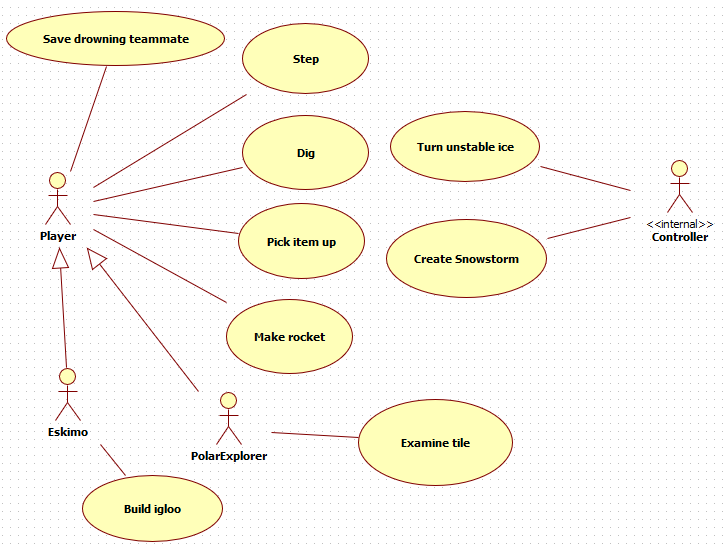
\includegraphics[width=17cm]{chapters/chapter02/use-case.png}
		\caption{Use-Case diagram}
		\label{fig:usecase}
	\end{center}
\end{figure}

\subsection{Use-case leírások}
%\comment{Minden use-case-hez külön}
\usecase{Step}{A játékos lép}{Player}{1. A játékos átlép egy másik jégtáblára. \newline 1.A A játékos telített instabil jégre lép, ami átfordul emiatt, a játékos vízbe esik. \newline 1.B A játékos lyukra lép, vízbe esik.}
\usecase{Dig}{A játékos ás}{Player}{1. A játékos eltávolít egy réteg havat a jégmezőről. \newline 1.A A játékos két réteg havat távolít el a jégmezőről a lapátja segítségével.}
\usecase{Pick item up}{A játékos felvesz egy tárgyat}{Player}{1. A játékos felvesz egy tárgyat. \newline 2. A tárgy a játékos tárgyai közt helyet foglal. \newline 2.A A játékos ételt vesz fel, ami növeli a testhőjét.}
\usecase{Make rocket}{Játékos megkísérli a játékot megnyerő rakéta összerakását}{Player}{1.A játékos és csapattársai sikeresen összerakják a rakétát és megnyerik a játékot. \newline 1.A A játékos és csapattársai nem rendelkeznek a megfelelő alkatrészekkel, vagy nem állnak egymáshoz elég közel és a rakéta nem épül össze.}
\usecase{Save drowning teammate}{Játékos megmenti fulladozó csapattársát}{Player}{1. A játékos dob egy kötelet fulladozó társának, megmentve őt.}
\usecase{Build igloo}{Eszkimó játékos iglut épít}{Eskimo}{1. Egy kiválasztott jégtáblára iglut épít az eszkimó.}
\usecase{Examine tile}{Sarkkutató játékos megnéz egy jégtáblát}{PolarExplorer}{1. Egy jégtábla teherbírását megnézi a sarkkutató}
\usecase{Turn unstable ice}{Túlterhelt, instabil jégtábla megfordul.}{Controller}{1. A túlterhelt jégtáblán lévő játékosok vízbe esnek \newline 2. A játékosok búvárruha vagy csapattárs segítsége miatt túlélik a vízbeesést. \newline 2.A Egy játékos nem éli túl a vízbe esést, a játék véget ér.}
\usecase{Create snowstorm}{Feltámad egy hóvihar}{Controller}{1. Egy hóvihar feltámad, ami néhány jégtáblán végigsöpör. \newline 2. A jégtáblákat hóval befedi, a játékosok testhőjét csökkenti a vihar.}

\section{Szótár}
%\comment{A szótár a követelmények alapján készítendő fejezet. Egy szótári bejegyzés definiálásához csak más szótári bejegyzések és köznapi – a feladattól független – fogalmak használhatók fel. A szótár mérete kb. 1-2 oldal legyen.}
\textbf{Alkatrész:} Jelzőrakéta összeszereléséhez szükséges tárgy. \\
\textbf{Átfordul (jégtábla):} Instabil jégtáblával történik, ha túl sokan  tartózkodnak rajta: A jégtáblán állók a vízbe esnek. \\
\textbf{Búvárruha:} Tárgy, túlélhető vele a vízbe esés. \\
\textbf{Elsütni (jelzőrakétát):} Tevékenység, jó esetben a játék megnyerése. \\
\textbf{Eltakarít (szereplő, havat):} Tevékenység, egy jégtábla hószintjének csökkentése. \\
\textbf{Építeni (iglut):} Tevékenység, iglu létrehozása. \\
\textbf{Eszkimó:} Osztály, képessége az iglu építés, kezdő testhője öt. \\
\textbf{Élelem:} Tárgy, testhő növelésére alkalmas. \\
\textbf{Fulladás:} Ha egy játékos a vízbe esik és nem segít rajta egy társa vagy nincs búvár ruhája, akkor megfullad (meghal). \\
\textbf{Felvesz (szereplő. tárgyat):} A szereplő egy tárgyat vagy elhelyez a saját tárgyai között. \\
\textbf{Hó:} Jégtábla tulajdonsága. \\
\textbf{Hóvihar:} Esemény, random következik be érinthet szereplőt vagy jégtáblát. \\
\textbf{Hóvihar elkap (jégtáblát):} A jégtáblát újra hó fedi be. \\
\textbf{Hóvihar elkap (szereplőt):} A szereplő testhője eggyel csökken. \\
\textbf{Iglu:} Játéktér eleme. Jégtáblán létezhet. Tartózkodhatnak benne szereplők. \\
\textbf{Instabil (jégtábla):} Olyan jégtáblák, amelyek átfordulnak, ha túl sokan vannak rajta. \\
\textbf{Játék:} Ez a szoftver. \\
\textbf{Jégmező:} A játéktér. \\
\textbf{Jégtábla:} A játéktér egy eleme. \\
\textbf{Jelzőfény:} Alkatrész a jelzőrakéta összerakásához. \\
\textbf{Jelzőrakéta:} Tárgy, a játék megnyeréséhez szükséges. \\
\textbf{Képesség:} Osztályra jellemző tevékenység. \\
\textbf{Kimenekíteni (szereplő, szereplőt):} Kötél segítségével egy szereplő ki tud menekíteni egy másik vízbe esett szereplőt. \\
\textbf{Kör:} Időegység, minden körben minden szereplő 4 munkát végezhet. \\
\textbf{Kötél:} Tárgy, vízbe esett játékos megmenthető vele. \\
\textbf{Lapát:} Tárgy, eltakarítható vele a hó a jégtáblákról. \\
\textbf{Lép (szereplő jégtáblára):} Tevékenység, amivel egy szereplő változtatni tudja a helyzetét. \\
\textbf{Lyuk:} A játéktér eleme. Jégtáblán létezhet, ha egy szereplő rááll, akkor vízbe esik. \\
\textbf{Meghal (szereplő):} Az az összes testhő egység elvesztése vagy fulladás, következménye a játék elvesztése. \\
\textbf{Megnézni (jégtáblát):} Sarkkutató képessége, megállapítja egy jégtábla teherbírását.
\textbf{Munka:} Egy szereplő által, egy körben végezhető tevékenységek száma. \\
\textbf{Osztály:} Szereplő fajta. \\
\textbf{Összeszerelni (jelzőrakétát):} Ha a szereplők megtalálják az összes alkatrészt és ugyan arra a jégtáblára helyezik őket, akkor hajthatják végre ezt a tevékenységet. \\
\textbf{Patron:} Alkatrész a jelzőrakéta összerakásához. \\
\textbf{Pisztoly:} Alkatrész  a jelzőrakéta összerakásához.\\
\textbf{Sarkkutató:} Osztály, képessége a jégtábla megnézése, kezdő testhője négy. \\
\textbf{Stabil (jégtábla):} Olyan jégtábla, amelyen akárhány szereplő állhat. \\
\textbf{Szereplő:} Egy játékos avatárja a játéktéren. \\
\textbf{Tárgy:} Entitás, létezhet jégtáblába fagyva, vagy szereplő birtokában. \\
\textbf{Tenger:} A játéktér eleme, körülveszi a jégmezőt. \\
\textbf{Tesszaláció:} Kétdimenziós síkon egy geometriai forma ismétlése átlapolás és rések nélkül.
\textbf{Testhő:} Szereplő tulajdonsága, ha elfogy akkor meghal. \\
\textbf{Tevékenység:} Egy szereplő megváltoztatja a játékteret. \\
\textbf{Tiszta (jégtábla):} Jégtábla, amin nincs hó. \\
\textbf{Vízbe esik (szereplő):} Akkor következhet be, ha az adott szereplő lyukra áll vagy átfordul alatta a jégtábla \\

\section{Projekt terv}
%\comment{Tartalmaznia kell a projekt végrehajtásának lépéseit, a lépések, eredmények határidejét, az egyes feladatok elvégzéséért felelős személyek nevét és beosztását, a szükséges erőforrásokat, stb. Meg kell adni a csoportmunkát támogató eszközöket, a választott technikákat! Definiálni kell, hogy hogyan történik a dokumentumok és a forráskód megosztása!}
\subsection{Végrehajtás lépései}
\begin{tabular}{|l|l|} \hline
	febr. 24. & Követelmény, projekt, funkcionalitás dokumentum elkészítése \\ \hline
	márc. 2.  & Analízis modell kidolgozása 1                                                                          \\ \hline
	márc. 9.  & Analízis modell kidolgozása 2                                                                          \\ \hline
	márc. 16. & Szkeleton tervezése                                                                                    \\ \hline
	márc. 23. & Szkeleton - beadás és a forráskód herculesre való feltöltése                                           \\ \hline
	márc. 30. & Prototípus koncepciójának elkészítése                                                                  \\ \hline
	ápr. 6.   & Részletes tervek elkészítése                                                                           \\ \hline
	ápr. 20.  & Prototípus készítése, tesztelése                                                                       \\ \hline
	ápr. 27.  & Prototípus - beadás és a forráskód, a tesztbemenetek és az elvárt kimenetek herculesre való feltöltése \\ \hline
	máj. 4.   & Grafikus felület specifikációja                                                                        \\ \hline
	máj. 18.  & Grafikus változat és Összefoglalás - beadás és a forráskód herculesre való feltöltése                  \\ \hline
\end{tabular}

\subsection{Beosztás}
Minden héten az aheti feladattal a csapat összes tagja dolgozni fog, különböző mértékben, ahogy a tagok ideje engedi. Az 5 fős csapat összetartásáért, és hogy elkészüljön a feladat a csapat vezetője, Kiss Andor a felelős. A dokumentumok nyomtatásáért minden héten beadás előtt megbeszéljük a felelőst. Az UML-es részekkel főleg Kiss Andor, a grafikával főleg Máté Botond tervez majd foglalkozni, de mindenki más is kiveszi a részét a dologból.

\subsection{Erőforrások:}
A tagok közti kommunikációt egy Facebook Messengeres beszélgetős csoportban csináljuk főleg, emellett persze előjöhet a projekt labor feladatainak témája amikor élőben találkozunk, akkor is, például előadáson, konzultáción, vagy egy közeli sörözőben.
A verziókezeléshez Git-et használunk, a fájlok és a tervek megosztásához Github-ot és Google Docs-ot használunk.
A dokumentációhoz \LaTeX-et és Microsoft Wordöt használunk.
Modellezéshez WhiteStarUML-t használunk.
Fejlesztőkörnyezetként IntelliJ-t vagy Eclipset használunk, ez a tagok egyéni preferenciája.
Fordításoz a fejlesztőkörnyezetet használjuk.

% Szoftprojlab
% ===========================================================================
%
\section{Napló}

\begin{naplo}

\bejegyzes{2020.02.12.~09:00~}{0,5 óra}{Lant}{GitHub repo előkészítése.}
\bejegyzes{2020.02.12.~21:30~}{0,5 óra}{Kiss}{Ötletelés.}
\bejegyzes{2020.02.13.~20:30~}{1 óra}{Kiss}{Ötletelés.}
\bejegyzes{2020.02.15.~17:30~}{15 perc}{Kiss}{Ötletelés.}
\bejegyzes{2020.02.19.~12:00~}{2 óra}{Mindenki}{Konzi.}
\bejegyzes{2020.02.21.~14:30~}{1,5 óra}{Kiss}{Use-case-ek.}
\bejegyzes{2020.02.21.~15.00~}{15 perc}{Lant}{Ötletelés.}
\bejegyzes{2020.02.22.~15:45~}{2,5 óra}{Glávits}{Doksi elkezdése.}
\bejegyzes{2020.02.23.~14:00~}{1,5 óra}{Kiss}{Követelmények megfogalmazása.}
\bejegyzes{2020.02.23.~15:30~}{1 óra}{Kiss}{Forgatókönyvek leírása.}
\bejegyzes{2020.02.23.~15:00~}{1,5 óra}{Glávits}{Szótár elkészítése.}
\bejegyzes{2020.02.23.~15:00~}{2 óra}{Konrád}{Szótár elkészítése.}
\bejegyzes{2020.02.23.~16:00~}{0,5 óra}{Máté}{Doksi formázás.}
\bejegyzes{2020.02.23.~16:30~}{1,5 óra}{Konrád}{Doksi formázás.}
\bejegyzes{2020.02.23.~16:30~}{1 óra}{Kiss}{Doksi javítás.}
\bejegyzes{2020.02.23.~20:00~}{0,5 óra}{Glávits}{Napló összeírás.}

\end{naplo}


%
\setcounter{chapter}{2}
% Szglab4
% ===========================================================================
%
\chapter{Analízis modell kidolgozása 1}

\thispagestyle{fancy}

\section{Objektum katalógus}

\subsection{Játékos}
Három vagy több van belőle. Körökre bontva teszik a dolgukat. Saját körükben tudnak mozogni, különböző tárgyakat használni vagy a speciális képességüket használni. A játék megnyeréséhez szükséges rakétapisztoly alkatrészek összegyűjétse a feladatuk. Ha vízbe esnek, vagy kihűlnek akkor a játéknak vége.

\subsection{Jégtábla}
Ilyenek alkotják a játékos számára a játékteret, ezeken lehet mozogni. Jégtáblák tartalmazhatnak tárgyakat amelyeket ki lehet ásni. Az instabil jégtábla képes vízbe ejteni a rajta állókat, ha túl sokan vannak. A jégtáblán lehet hó. Néha lehet rajta hóvihar, mely csökkenti a rajta állók testhőjét

\subsection{Kötél}
Ennek segítésével ki lehet húzni egy vízbe esett játékost.

\subsection{Búvárruha}
A jétékos képes a vízben is mozogni vele, illetve nem veszít testhőt ha vízben tartózkodik.

\subsection{Lapát}
Segítségével 2 egységnyi hó takarítható el a egy adott tábláról.

\subsection{Élelem}
Ha a játékos elfogyasztja a testhője 1-el megnő.

\subsection{Rakétapisztoly Alkatrész}
A játékban 3 darab ilyen megtalálása vezet a játék sikeres befejezéséhez. Az összeszereléshez mindháromnak egy helyen kell lennie.

\subsection{Iglu}
Eszkimó (Játékos) képes építeni, itt átvészelhetőek a hóviharok

\section{Statikus struktúra diagramok}
\comment{Az előző alfejezet osztályainak kapcsolatait és publikus metódusait bemutató osztálydiagram(ok). Tipikus hibalehetőségek: csillag-topológia, szigetek.}

\begin{figure}[h]
\begin{center}
%\includegraphics[width=17cm]{chapters/chapter03/example.pdf}
\caption{x}
\label{fig:example1}
\end{center}
\end{figure}


\section{Osztályok leírása}
\comment{Az előző alfejezetben tárgyalt objektumok felelősségének formalizálása attribútumokká, metódusokká. Csak publikus metódusok szerepelhetnek. Ebben az alfejezetben megjelennek az interfészek, az öröklés, az absztrakt osztályok. Segédosztályokra még mindig nincs szükség. Az osztályok ABC sorrendben kövessék egymást. Interfészek esetén az Interfészek, Attribútumok pontok kimaradnak.}

\subsection{Osztály1}
\begin{itemize}
\item Felelősség\\
\comment{Mi az osztály felelőssége. Kb 1 bekezdés.}
\item Ősosztályok\\
\comment{Mely osztályokból származik (öröklési hierarchia)\newline
Legősebb osztály $\rightarrow$ Ősosztály2 $\rightarrow$ Ősosztály3...}
\item Interfészek\\
\comment{Mely interfészeket valósítja meg.}
\item Attribútumok\\
\comment{Milyen attribútumai vannak}
	\begin{itemize}
		\item attribútum1: attribútum jellemzése: mire való
		\item attribútum2: attribútum jellemzése: mire való
	\end{itemize}
\item Metódusok\\
\comment{Milyen publikus metódusokkal rendelkezik. Metódusonként egy-három mondat arról, hogy a metódus mit csinál.}
	\begin{itemize}
		\item int foo(Osztály3 o1, Osztály4 o2): metódus leírása
		\item int bar(Osztály5 o1): metódus leírása
	\end{itemize}
\end{itemize}

\subsection{Osztály2}
\begin{itemize}
\item Felelősség\\
\comment{Mi az osztály felelőssége. Kb 1 bekezdés.}
\item Ősosztályok\\
\comment{Mely osztályokból származik (öröklési hierarchia)\newline
Legősebb osztály $\rightarrow$ Ősosztály2 $\rightarrow$ Ősosztály3...}
\item Interfészek\\
\comment{Mely interfészeket valósítja meg.}
\item Attribútumok\\
\comment{Milyen attribútumai vannak}
	\begin{itemize}
		\item attribútum1: attribútum jellemzése: mire való
		\item attribútum2: attribútum jellemzése: mire való
	\end{itemize}
\item Metódusok\\
\comment{Milyen publikus metódusokkal rendelkezik. Metódusonként egy-három mondat arról, hogy a metódus mit csinál.}
	\begin{itemize}
		\item int foo(Osztály3 o1, Osztály4 o2): metódus leírása
		\item int bar(Osztály5 o1): metódus leírása
	\end{itemize}
\end{itemize}

\section{Statikus struktúra diagramok}
\comment{Az előző alfejezet osztályainak kapcsolatait és publikus metódusait bemutató osztálydiagram(ok). Tipikus hibalehetőségek: csillag-topológia, szigetek.}

\begin{figure}[h]
\begin{center}
%\includegraphics[width=17cm]{chapters/chapter03/example.pdf}
\caption{x}
\label{fig:example1}
\end{center}
\end{figure}

\section{Szekvencia diagramok}
\comment{Inicializálásra, use-case-ekre, belső működésre. Konzisztens kell legyen az előző alfejezettel. Minden metódus, ami ott szerepel, fel kell tűnjön valamelyik szekvenciában. Minden metódusnak, ami szekvenciában szerepel, szereplnie kell a valamelyik osztálydiagramon.}

\begin{figure}[h]
\begin{center}
%\includegraphics[width=17cm]{chapters/chapter03/example.pdf}
\caption{x}
\label{fig:example2}
\end{center}
\end{figure}

\section{State-chartok}
\comment{Csak azokhoz az osztályokhoz, ahol van értelme. Egyetlen állapotból álló state-chartok ne szerepeljenek. A játék működését bemutató state-chart-ot készíteni tilos.}

\begin{figure}[h]
\begin{center}
%\includegraphics[width=17cm]{chapters/chapter03/example.pdf}
\caption{x}
\label{fig:example3}
\end{center}
\end{figure}


% Szglab4
% ===========================================================================
%
\section{Napló}

\begin{naplo}

\bejegyzes{2020.02.24.~08:30~}{1 óra}{Kiss}{Class diagram rajzolás}
\bejegyzes{2020.02.24.~14:00~}{1,5 óra}{Lant}{Ami kimaradt az első leadásból, use-caseknek}
\bejegyzes{2020.02.24.~13:00~}{2 óra}{Kiss}{Szekvencia diagram rajzolás}
\bejegyzes{2020.02.25.~09:30~}{1 óra}{Kiss}{Szekvencia diagram rajzolás}
\bejegyzes{2020.02.25. 15:00}{0.5 óra}{Kiss}{Tervezés ötletelés TODO megírása.}
\bejegyzes{2020.02.23. 16:00}{1 óra}{Glávits}{Class diagram ellenőrzés.}
\bejegyzes{2020.02.25. 18.25}{1 óra}{Lant}{Class diagram ellenőrzés.}
\bejegyzes{2020.02.23. 22:45}{2 óra}{Glávits}{Class diagram javítás}
\bejegyzes{2020.02.20. 19:00}{2 óra}{Kiss}{ötletelés}
\bejegyzes{2020.02.20. 19:00}{2 óra}{Glávits}{ötletelés}
\bejegyzes{2020.02.20. 20:45}{2 óra}{Glávits}{class diagram}
\bejegyzes{2020.02.29. }{reggeltől estig}{Lant \newline Glávits \newline Kiss}{ötletelés a class diagramról}
\bejegyzes{2020.02.29. 22.00}{20 perc}{Lant}{objektum jegyzék}
\bejegyzes{2020.03.01. 11:00}{1 óra}{Glávits}{osztály jegyzék írása}
\bejegyzes{2020.03.01. 14:00}{2 óra}{Glávits}{szekvencia}
\bejegyzes{2020.03.01. 14:00,}{2 óra}{Kiss}{szekvencia}
\bejegyzes{2020.03.01.~16:00~}{4 óra}{Máté}{Szekvencia diagram készítés}
\bejegyzes{2020.03.01. 18:00}{3 óra}{Konrád}{szekvencia}
\bejegyzes{2020.03.01. 18.00}{2 óra}{Lant}{class diagram leírások}
\bejegyzes{2020.03.01, 19:00}{5 óra}{Glávits \newline Kiss}{minden szart csinál}
\bejegyzes{2020.03.01.~20:30~}{1 óra}{Máté}{Szekvencia diagram javítás}
\bejegyzes{2020.03.01.~22:00~}{2 óra}{Konrád}{Dokumentum szerkesztés}
\bejegyzes{2020.03.01.~23:30~}{2,5 óra}{Máté}{Dokumentum formázás}
\bejegyzes{2020.03.02.~00:00~}{45 perc}{Glávits}{Typo-k javítása}

\end{naplo}


%
\setcounter{chapter}{3}
% Szoftprojlab
% ===========================================================================
%
\chapter{Analízis modell kidolgozása 1}

\thispagestyle{fancy}

\section{Objektum katalógus}

\subsection{Játékos}
Három vagy több van belőle. Körökre bontva teszik a dolgukat. Saját körükben tudnak mozogni, különböző tárgyakat használni vagy a speciális képességüket használni. A játék megnyeréséhez szükséges rakétapisztoly alkatrészek összegyűjétse a feladatuk. Ha vízbe esnek, vagy kihűlnek akkor a játéknak vége.

\subsection{Jégtábla}
Ilyenek alkotják a játékos számára a játékteret, ezeken lehet mozogni. Jégtáblák tartalmazhatnak tárgyakat amelyeket ki lehet ásni. Az instabil jégtábla képes vízbe ejteni a rajta állókat, ha túl sokan vannak. A jégtáblán lehet hó. Néha lehet rajta hóvihar, mely csökkenti a rajta állók testhőjét

\subsection{Kötél}
Ennek segítésével ki lehet húzni egy vízbe esett játékost.

\subsection{Búvárruha}
A játékos képes a vízben is mozogni vele, illetve nem veszít testhőt ha vízben tartózkodik.

\subsection{Lapát}
Segítségével 2 egységnyi hó takarítható el, egy egység munkával.

\subsection{Élelem}
Ha a játékos elfogyasztja, a testhője 1-el megnő.

\subsection{Rakétapisztoly Alkatrész}
A játékban 3 darab ilyen megtalálása vezet a játék sikeres befejezéséhez. Az összeszereléshez mindháromnak egy helyen kell lennie.

\subsection{Iglu}
Eszkimó (Játékos) képes építeni, itt átvészelhetőek a hóviharok.

\newpage
\section{Statikus struktúra diagramok}
%\comment{Az előző alfejezet osztályainak kapcsolatait és publikus metódusait bemutató osztálydiagram(ok). Tipikus hibalehetőségek: csillag-topológia, szigetek.}

%\begin{figure}[h]
%\begin{center}
%\includegraphics[width=17cm]{chapters/chapter03/example.pdf}
%\caption{x}
%\label{fig:example1}
%\end{center}
%\end{figure}


\section{Osztályok leírása}
%\comment{Az előző alfejezetben tárgyalt objektumok felelősségének formalizálása attribútumokká, metódusokká. Csak publikus metódusok szerepelhetnek. Ebben az alfejezetben megjelennek az interfészek, az öröklés, az absztrakt osztályok. Segédosztályokra még mindig nincs szükség. Az osztályok ABC sorrendben kövessék egymást. Interfészek esetén az Interfészek, Attribútumok pontok kimaradnak.}

\subsection{BareHands}
\begin{itemize}
\item A játékos így ás, ha nincs ásója.

\item Interfészek:
	\begin{itemize}
		\item DigStrategy
	\end{itemize}

\item Metódusok:
	\begin{itemize}
		\item bool Dig(Tile t): Csökkenti a tile-on található hó mennyiségét (int)
	\end{itemize}
\end{itemize}

\subsection{BareIce}
\begin{itemize}
\item A jégtáblán nincs védelem a vihar elől.

\item Interfészek:

	\begin{itemize}
		\item ChillStormStrategy
	\end{itemize}

\item Metódusok:
	\begin{itemize}
		\item void Chill(Tile t): Táblán alló játékosok testhője csökken.
	\end{itemize}
\end{itemize}

\subsection{CantRescue}
\begin{itemize}
	\item A játékos nem tudja kihúzni a csapattársát.
	
\item Interfészek:
\begin{itemize}
	\item RescueStrategy
\end{itemize}

\item Metódusok:
\begin{itemize}
	\item void Rescue(Tile water, Tile land): üres
\end{itemize}
\end{itemize}

\subsection{ChillStormStrategy}
\begin{itemize}
	\item A jégtábla így hűti viharban a játékosokat.

	\item Metódusok:
	\begin{itemize}
		\item abstract void Chill(Tile t)
	\end{itemize}
\end{itemize}

\subsection{ChillWaterStrategy}
\begin{itemize}
	\item A jégtábla így hűti a vízbe esett játékosokat.
	
\item Metódusok:
\begin{itemize}
	\item abstract void Chill(Tile t)
\end{itemize}
\end{itemize}

\subsection{DigStrategy}
\begin{itemize}
	\item A játékos így ás.
	
\item Metódusok:
\begin{itemize}
	\item abstract bool Dig(Tile t)
\end{itemize}
\end{itemize}

\subsection{DryLand}
\begin{itemize}
	\item A szárazföld nem hűti a játékosokat.
	
\item Interfészek:
	\begin{itemize}
		\item ChillWaterStrategy
	\end{itemize}
\item Metódusok:
\begin{itemize}
	\item void Chill(Tile t): üres
\end{itemize}
\end{itemize}

\subsection{Empty}
\begin{itemize}
	\item Nincs jégbe fagyott tárgy.
	
\item Interfészek:
	\begin{itemize}
		\item GiveItemStrategy
	\end{itemize}
\item Metódusok
\begin{itemize}
	\item void GiveTo(Player p): üres
\end{itemize}
\end{itemize}

\subsection{Eskimo}
\begin{itemize}
	\item Játékos osztály.
	
	\item Ősosztályok:
	\begin{itemize}
		\item Player
	\end{itemize}
\item Metódusok:
\begin{itemize}
	\item void BuildIgloo(): Épít egy iglut a mezőre, amin áll.
\end{itemize}
\end{itemize}

\subsection{Food}
\begin{itemize}
	\item Élelem, amit a játékos meg tud enni, hogy növelje a testhőjét.
	
\item Interfészek:
\begin{itemize}
	\item GiveItemStrategy
\end{itemize}

\item Metódusok:
\begin{itemize}
	\item void GiveTo(Player p): A játékos kap egy élelmet.
\end{itemize}
\end{itemize}

\subsection{FoodStore}
\begin{itemize}
	\item A játékos ebben a zsebben tárolja az élelmet.

\item Attribútumok:

\begin{itemize}
	\item count: int: Hány élelem van a játékosnál

\end{itemize}
\item Metódusok:
\begin{itemize}
	\item void feed(Player p): Játékos testhője megnő.
\end{itemize}
\end{itemize}

\subsection{Game}
\begin{itemize}
	\item Interface a Model és a Controller között. A játékmesterhez tartozó működést valósítja meg.
	
\item Attribútumok:

\begin{itemize}
	\item players: Player[3..*]: Tárolja a játékosokat
	\item icefield: Tile[1..*]: Tárolja a pályát alkotó elemeket
\end{itemize}
\item Metódusok:
\begin{itemize}
	\item Tile CreateIce(): Létrehoz egy jégtáblát. Ez a metódus az init szekvencia része.
	\item Tile CreateUnstableIce(): Létrehoz egy instabil jégtáblát. Ez a metódus az init szekvencia része.
	\item Tile CreateSea(): Létrehoz egy vizet. Ez a metódus az init szekvencia része.
	\item Tile CreateHole(): Létrehoz egy lyukat: olyan vizet amit hó fed. Ez a metódus az init szekvencia része.
	\item Player CreateEskimo(): Létrehoz egy eszkimó játékost. Ez a metódus az init szekvencia része.
	\item Player CreatePolarExplorer(): Létrehoz egy sarkkutató játékost. Ez a metódus az init szekvencia része.
	\item void GameOver(): Ha vége a játéknak, szól a Controllernek, hogy vesztettünk. Külső metódus.
	\item void Turn(): Ezt a metódust a Controller hívja körönként. 
	\item void Victory(): Ha vége a játéknak, szól a Controllernek, hogy nyertünk. Külső metódus.
\end{itemize}
\end{itemize}

\subsection{Igloo}
\begin{itemize}
	\item Ezen a jégtáblán iglu áll, a játékosok védve vannak a vihartól.
	
\item Interfészek:
\begin{itemize} 
	\item ChillStromStrategy
\end{itemize}
\item Metódusok:
\begin{itemize}
	\item void Chill(Tile t): üres
\end{itemize}
\end{itemize}

\subsection{Naked}
\begin{itemize}
	\item A játékos védtelen a hideg vízzel szemben.
	
\item Interfészek:
\begin{itemize}
	\item WaterResistanceStrategy
\end{itemize}
\item Metódusok:
\begin{itemize}
	\item void Chill(Player p): Játékosnak nincsen ereje a vízben úszni búvárruha nélkül.
\end{itemize}
\end{itemize}

\subsection{Part}
\begin{itemize}
	\item Jégbefagyott alkatrész.

\item Interfészek:
\begin{itemize}
	\item GiveItemStrategy
\end{itemize}

\item Metódusok:
\begin{itemize}
	\item void GiveTo(Player p): A játékos tárolójába kerül egy darab a rakétapisztolyból.
\end{itemize}
\end{itemize}

\subsection{PartStore}
\begin{itemize}
	\item A játékos ebben a zsebben tárolja az alkatrészeket.
	
\item Attribútumok:
\begin{itemize}
	\item count: int: Hány darab alkatrész van belőle a játékosnál?
\end{itemize}
\item Metódusok:
\begin{itemize}
	\item void Gain(PartStore ps): Átveszi az alkatrészeket.
	\item void Gain(int n): Megnő az alkatrészek száma ami a játékosnál van.
\end{itemize}
\end{itemize}

\subsection{Player}
\begin{itemize}
	\item Játékos osztály, amit a felhasználó irányít a grafikus felületen keresztül.

\item Attribútumok:
\begin{itemize}
	\item bodyTemp: int: Jelzi a játékos jelenlegi hőmérsékletét, ha 0 akkor megfagy $\rightarrow$ játék vége.
	\item currentTile: Tile: A játékos ismeri a mezőt amin éppen áll.
	\item digStrategy: DigStrategy: Eldönti hogyan képes ásni a játékos.
	\item energy: int: Számlálja mennyit mozogott az adott körben a játékos.
	\item foodStore: FoodStore: Tárolja a játékos ételeit.
	\item partStore: PartStore: Tárolja a játékos rakéta alkatrészeit.
	\item rescueStrategy: RescueStrategy: Eldönti, hogy megmenthet egy játékos egy másikat a vízbeesés után.
	\item waterResistanceStrategy: WaterResistanceStrategy: Eldönti, hogy a játékos hogyan viselkedik vízbeesés esetén.
\end{itemize}
\item Metódusok:
\begin{itemize}
	\item void AssembleFlare(): Összerakja a játék végéhez szükséges rakéta pisztolyt. 1 munkaegység
	\item void Chill(): A testhő 1-el csökken, ha 0 alá megy GameOver.
	\item void DecrementEnergy(): Az energiát csökkentő helper metódus.
	\item void Dig(): Ezt a metódust a Controller hívja. A játékos havat ás. 1 munkaegység
	\item void EatFood(): Ezt a metódust a Controller hívja. A játékos eszik.
	\item void PickUp(): Ezt a metódust a Controller hívja. A játékos felvesz egy tárgyat. 1 munkaegység
	\item void PlaceOn(Tile t): Init szekvencia része. RopeRescue szekvencia része. Rárak egy játékost egy másik Tile-ra.
	\item void RescueTeammate(direction d): Ezt a metódust a Controller hívja. A játékos kiment egy másikat a vízből. 1 munkaegység
	\item void ResistWater(): A játékos testhője a WaterResistance szerint változik.
	\item void Step(): Ezt a metódust a Controller hívja. A játékos lép, ha van még hozzá elég energiája. 1 munkaegység
	\item void ToFoodStore(): Élelem megtalálásához helper metódus.
\end{itemize}
\end{itemize}


\subsection{PolarExplorer}
\begin{itemize}
	\item Játékos típus, akivel valaki játszhat
	
	\item Ősosztályok:
	\begin{itemize}
		\item Player
	\end{itemize}

\item Metódusok:
\begin{itemize}
	\item int Examine(direction d): A játékos megnézheti, hogy egy adott Tile-nak mennyi a teherbírása.
\end{itemize}
\end{itemize}

\subsection{RescueStrategy}
\begin{itemize}
	\item A játékos így húzza ki csapattársát a vízből.\

\item Metódusok:
\begin{itemize}
	\item abstract void Rescue(Tile water, Tile land): üres
\end{itemize}
\end{itemize}

\subsection{Rope}
\begin{itemize}
	\item Jégbe fagyott kötél.
\item Interfészek:
\begin{itemize}
	\item GiveItemStrategy
\end{itemize}
\item Metódusok
\begin{itemize}
	\item void GiveTo(Player p): Felrhuázza a játékost kötéllel.
\end{itemize}
\end{itemize}

\subsection{RopeRescue}
\begin{itemize}
	\item A játékos kihúzza csapattársát a vízből.
\item Interfészek:
\begin{itemize}
	\item RescueStrategy
\end{itemize}

\item Metódusok:
\begin{itemize}
	\item void Rescue(Tile water, Tile land): A vízben lévők közül egyvalaki rákerül a kihúzó játékos cellájára.
\end{itemize}
\end{itemize}

\subsection{ScubaGear}
\begin{itemize}
	\item Jégbe fagyott búvárruha.
\item Interfészek:
\begin{itemize}
	\item GiveItemStrategy
\end{itemize}
\item Metódusok:
\begin{itemize}
	\item void GiveTo(): Felruházza a játékost búvárruhával.
\end{itemize}
\end{itemize}

\subsection{Sea}
\begin{itemize}
	\item Ez a cella tenger, hűti a játékosokat.
\item Interfészek:
\begin{itemize}
	\item ChillWaterStrategy
\end{itemize}

\item Metódusok:
\begin{itemize}
	\item void Chill(Tile t): Minden rajta álló testhője csökken a WaterResistanceStrategy szerint.
\end{itemize}
\end{itemize}

\subsection{ShovelDig}
\begin{itemize}
	\item Egyszer lehet ásni vele fáradság nélkül is.
\item Interfészek:
\begin{itemize}
	\item DigStrategy
\end{itemize}

\item Attribútumok:
\begin{itemize}
	\item lastUsed: bool: Volt-e már használva a körben
\end{itemize}
\item Metódusok:
\begin{itemize}
	\item void Dig(Tile t): Csökkenti a tile-on található hó mennyiségét.
\end{itemize}
\end{itemize}

\subsection{Tile}
\begin{itemize}
	\item Cella, ilyenekből áll a jégmező ahol a játékosok játszanak.
\item Attribútumok:
\begin{itemize}
	\item chillStormStrategy: ChillStormStrategy: Eldönti, kinek változik a testhője vihar esetén.
	\item chillWaterStrategy: ChillWaterStrategy: Eldönti, kinek változik a testhője víz esetén.
	\item giveItemStrategy: GiveItemStrategy: Eldönti, milyen tárgyat vesz fel a találó.
	\item neighborTiles: Tile[*]: Szomszédos cellákat ismer.
	\item occupants: Player[*]: Rajta lévő játékosok.
	\item snow: int: Rajta lévő hómennyiség.
	\item weightLimit: int: Rajta lévő játékosok számának maximuma.
	
\end{itemize}
\item Metódusok:
\begin{itemize}
	\item void ChillStorm(): Ezt a metódust a Controller hívja viharban. Hűti a játékosokat, ha nincsenek igluban.
	\item void ChillWater(): Ezt a metódust a Controller hívja körönként. Hűti a játékosokat, ha ez a cella víz.
	\item void DecrementSnow(): A hómennyiséget csökkentő helper függvény.
	\item void GiveItem(Player): A játékos megkapja a tartalmazott tárgyat.
	\item Tile NeighborAt(direction): Visszaadja az adott irányban szomszédos cellát.
	\item StepOn(Player): Játékos rálép a cellára, ha többen vannak mint a korlát, a jégtábla átfordul.
	\item StepOff(Player): Járékos lelép a celláról.
\end{itemize}
\end{itemize}

\subsection{WaterResistanceStrategy}
\begin{itemize}
	\item Így reagál a játékos a hideg vízre.
\item Metódusok:
\begin{itemize}
	\item abstract void Chill(Player p): üres
\end{itemize}
\end{itemize}


\section{Statikus struktúra diagramok}
%\comment{Az előző alfejezet osztályainak kapcsolatait és publikus metódusait bemutató osztálydiagram(ok). Tipikus hibalehetőségek: csillag-topológia, szigetek.}

%OSZTALY DIAGRAM IDE!!!!!

\begin{figure}[H]
	\begin{center}
		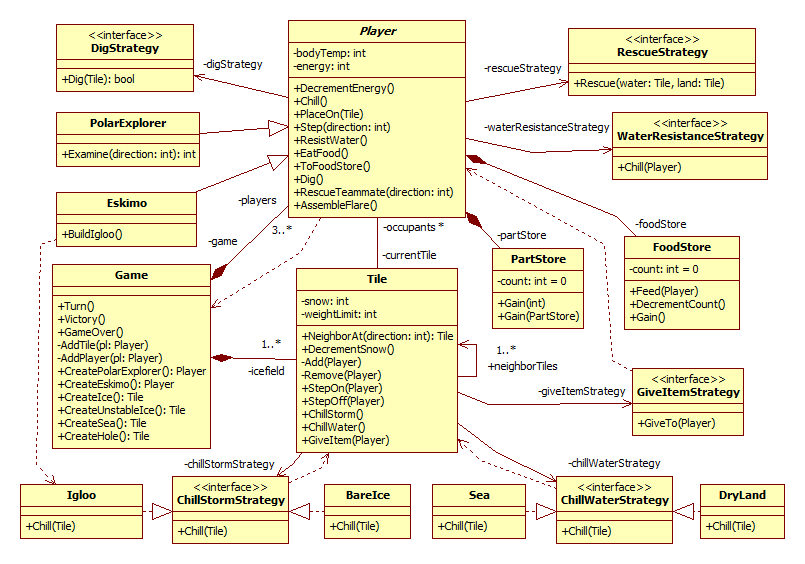
\includegraphics[angle=90, scale=0.76]{chapters/chapter03/ClassDiagramPart1.png}
		\caption{Osztálydiagram 1.}
		\label{fig:OsztalyDiagramPart1}
	\end{center}
\end{figure}
\begin{figure}[H]
	\begin{center}
		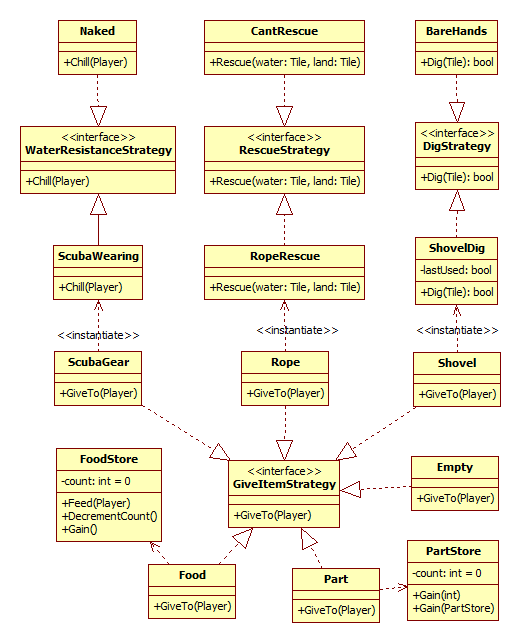
\includegraphics[width=17cm]{chapters/chapter03/ClassDiagramPart2.png}
		\caption{Osztálydiagram 2.}
		\label{fig:OsztalyDiagramPart2}
	\end{center}
\end{figure}

%\begin{figure}[h]
%\begin{center}
%\includegraphics[width=17cm]{chapters/chapter03/example.pdf}
%\caption{x}
%\label{fig:example1}
%\end{center}
%\end{figure}
\newpage
\section{Szekvencia diagramok}
%\comment{Inicializálásra, use-case-ekre, belső működésre. Konzisztens kell legyen az előző alfejezettel. Minden metódus, ami ott szerepel, fel kell tűnjön valamelyik szekvenciában. Minden metódusnak, ami szekvenciában szerepel, szereplnie kell a valamelyik osztálydiagramon.}
%find . -printf "\\\begin{figure}[H]\n\t\\\begin{center}\n\t\t\\\includegraphics[width=10cm]{chapters/chapter03/seqdiag/%f}\n\t\t\\\caption{aaa}\n\t\t\\\label{bbb}\n\t\\\end{center}\n\\\end{figure}\n"

\begin{figure}[H]
	\begin{center}
		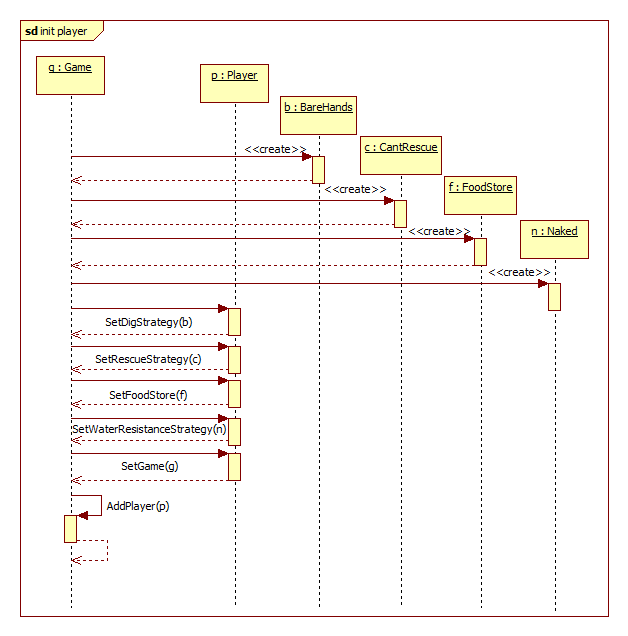
\includegraphics[width=15cm]{chapters/chapter03/seqdiag/Game_init_player.png}
		\caption{Game.InitPlayer()}
		\label{fig:GameInitPlayer}
	\end{center}
\end{figure}
\begin{figure}[H]
	\begin{center}
		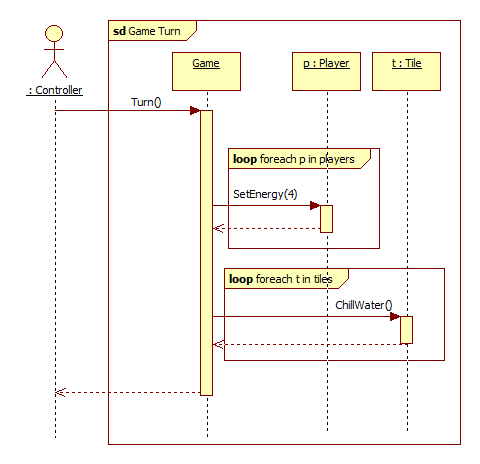
\includegraphics[width=10cm]{chapters/chapter03/seqdiag/Game_Turn.png}
		\caption{Game.Turn()}
		\label{fig:GameTurn}
	\end{center}
\end{figure}
\begin{figure}[H]
	\begin{center}
		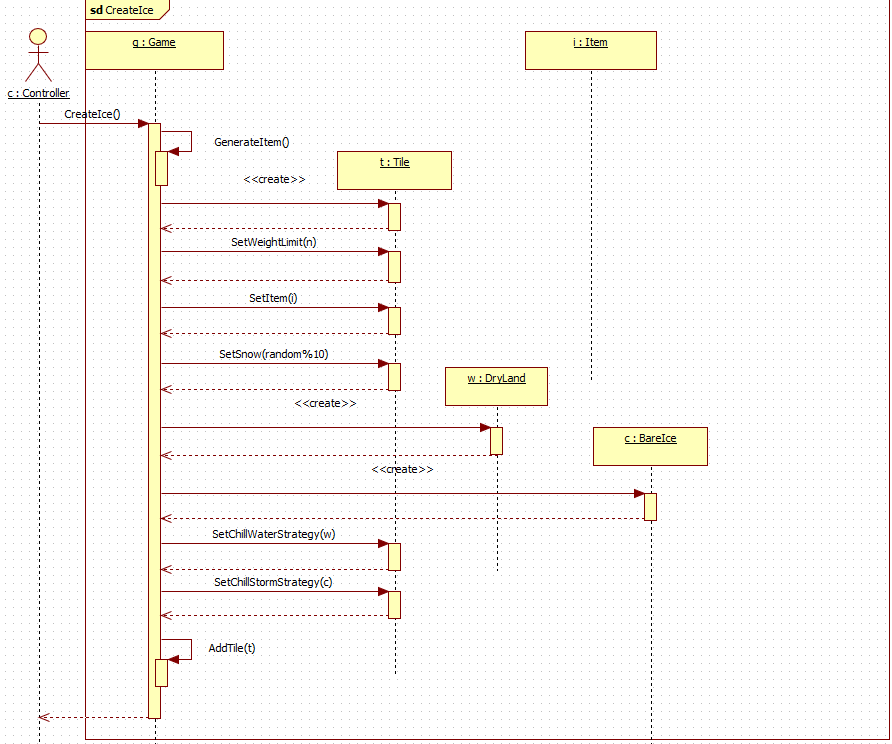
\includegraphics[width=15cm]{chapters/chapter03/seqdiag/Game_CreateIce.png}
		\caption{Game.CreateIce()}
		\label{fig:GameCreateIce}
	\end{center}
\end{figure}
\begin{figure}[H]
	\begin{center}
		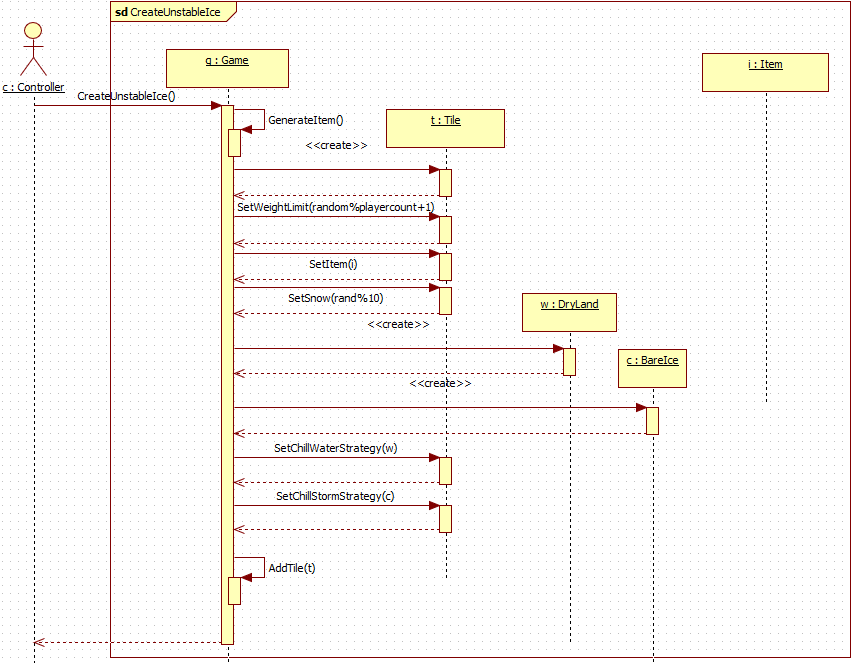
\includegraphics[width=17cm]{chapters/chapter03/seqdiag/Game_CreateUnstableIce.png}
		\caption{Game.CreateUnstableIce()}
		\label{fig:GameCreateUnstableIce}
	\end{center}
\end{figure}
\begin{figure}[H]
	\begin{center}
		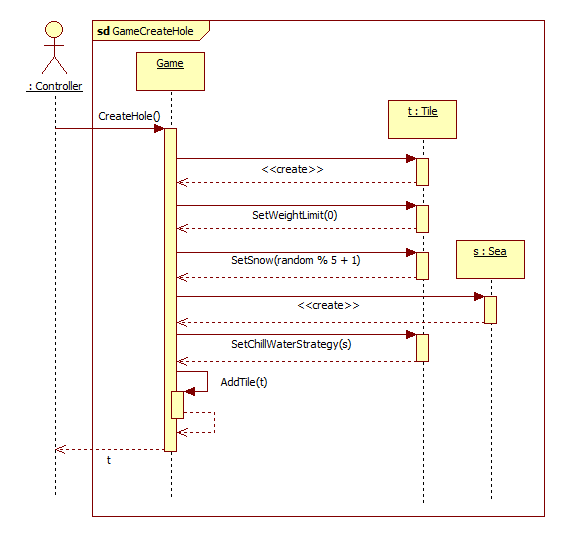
\includegraphics[width=15cm]{chapters/chapter03/seqdiag/Game_CreateHole.png}
		\caption{Game.CreateHole()}
		\label{fig:GameCreateHole}
	\end{center}
\end{figure}
\begin{figure}[H]
	\begin{center}
		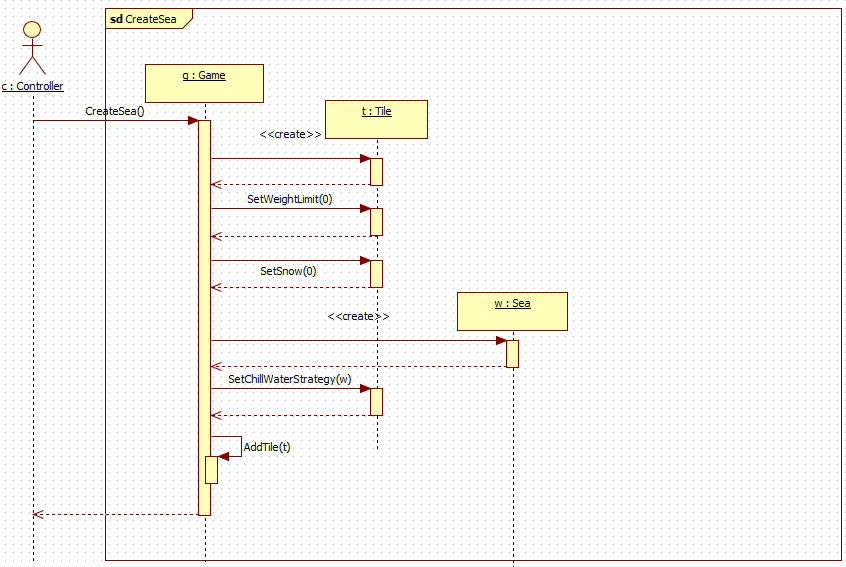
\includegraphics[width=13cm]{chapters/chapter03/seqdiag/Game_CreateSea.png}
		\caption{Game.CreateSea()}
		\label{fig:GameCreateSea}
	\end{center}
\end{figure}
\begin{figure}[H]
	\begin{center}
		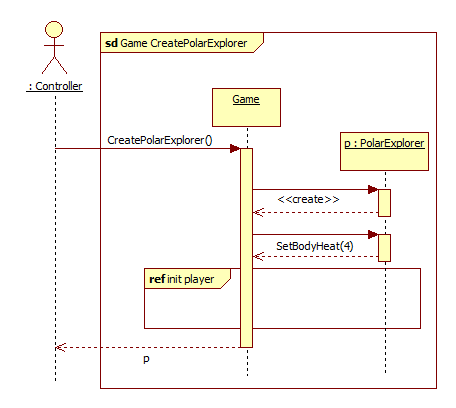
\includegraphics[width=10cm]{chapters/chapter03/seqdiag/Game_CreatePolarExplorer.png}
		\caption{Game.CreatePolarExplorer()}
		\label{fig:GameCreatePolarExplorer}
	\end{center}
\end{figure}
\begin{figure}[H]
	\begin{center}
		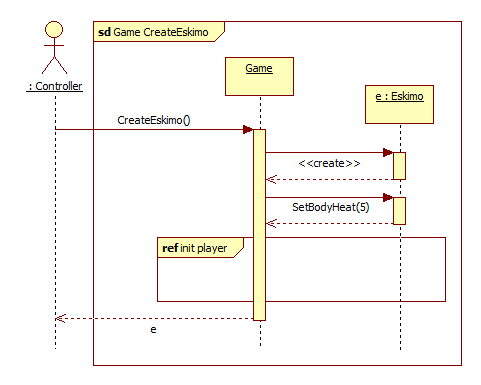
\includegraphics[width=10cm]{chapters/chapter03/seqdiag/Game_CreateEskimo.png}
		\caption{Game.CreateEskimo()}
		\label{fig:GameCreateEskimo}
	\end{center}
\end{figure}
\begin{figure}[H]
	\begin{center}
		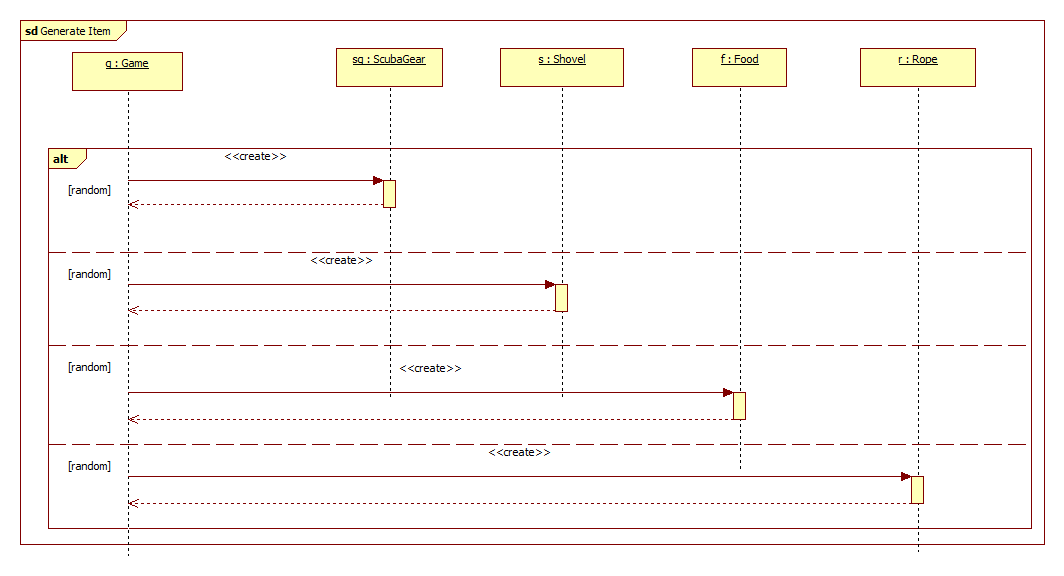
\includegraphics[width=17cm]{chapters/chapter03/seqdiag/Game_generate_item.png}
		\caption{Game.GenerateItem()}
		\label{fig:GameGenerateItem}
	\end{center}
\end{figure}
\begin{figure}[H]
	\begin{center}
		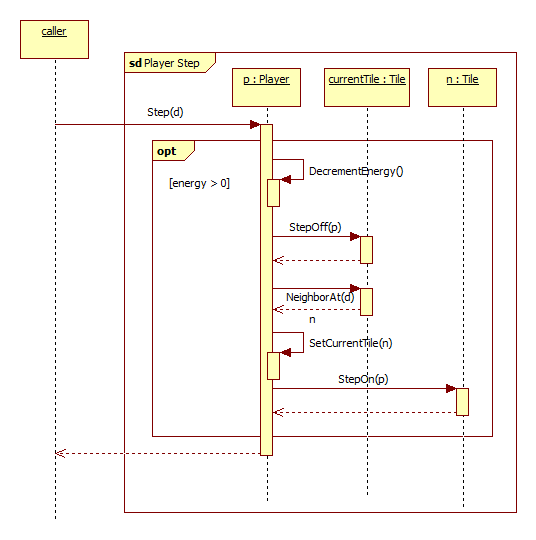
\includegraphics[width=11cm]{chapters/chapter03/seqdiag/Player_Step.png}
		\caption{Player.Step(direction: int)}
		\label{fig:PlayerStep}
	\end{center}
\end{figure}
\begin{figure}[H]
	\begin{center}
		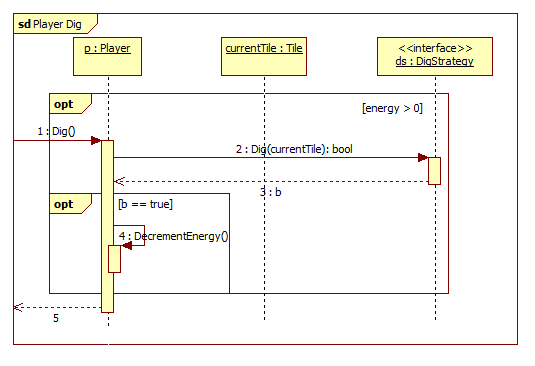
\includegraphics[width=15cm]{chapters/chapter03/seqdiag/Player_Dig.png}
		\caption{Player.Dig()}
		\label{fig:PlayerDig}
	\end{center}
\end{figure}
\begin{figure}[H]
	\begin{center}
		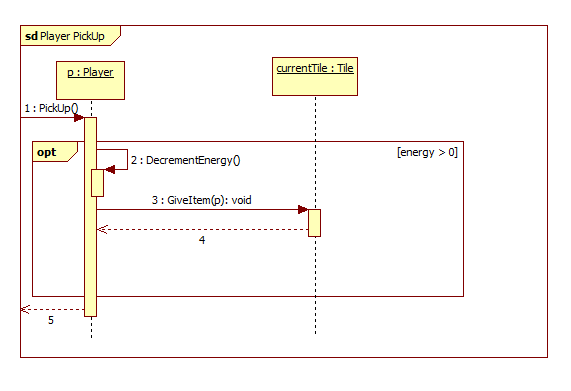
\includegraphics[width=15cm]{chapters/chapter03/seqdiag/Player_PickUp.png}
		\caption{Player.PickUp()}
		\label{fig:PlayerPickUp}
	\end{center}
\end{figure}
\begin{figure}[H]
	\begin{center}
		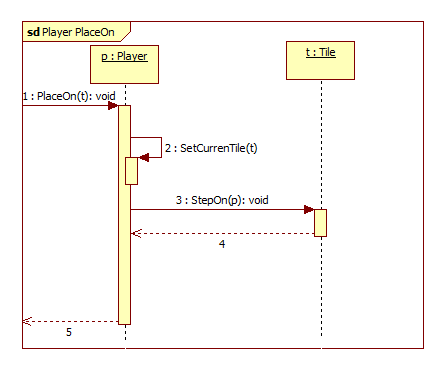
\includegraphics[width=10cm]{chapters/chapter03/seqdiag/Player_PlaceOn.png}
		\caption{Player.PlaceOn(Tile)}
		\label{fig:PlayerPlaceOn}
	\end{center}
\end{figure}
\begin{figure}[H]
	\begin{center}
		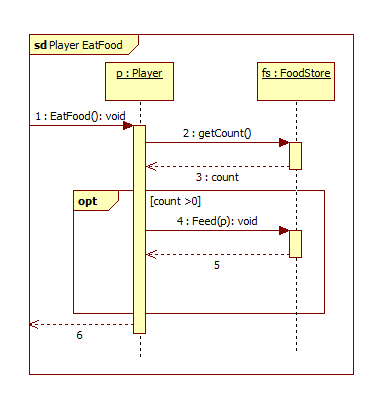
\includegraphics[width=10cm]{chapters/chapter03/seqdiag/Player_EatFood.png}
		\caption{Player.EatFood()}
		\label{fig:PlayerEatFood}
	\end{center}
\end{figure}
\begin{figure}[H]
	\begin{center}
		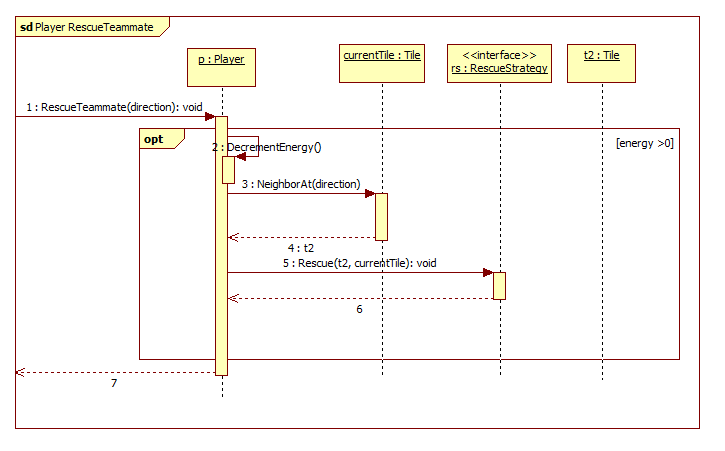
\includegraphics[width=15cm]{chapters/chapter03/seqdiag/Player_RescueTeammate.png}
		\caption{Player.RescueTeammate(direction: int)}
		\label{fig:Player.RescueTeammate}
	\end{center}
\end{figure}
\begin{figure}[H]
	\begin{center}
		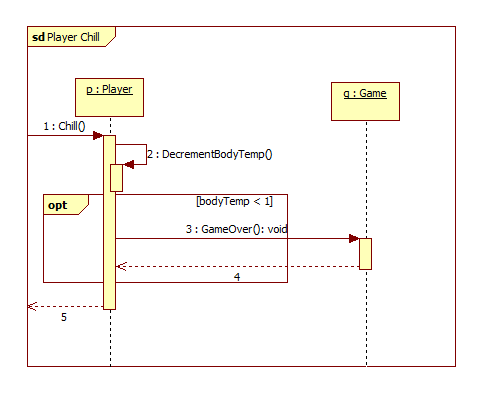
\includegraphics[width=10cm]{chapters/chapter03/seqdiag/Player_Chill.png}
		\caption{Player.Chill()}
		\label{fig:PlayerChill}
	\end{center}
\end{figure}
\begin{figure}[H]
	\begin{center}
		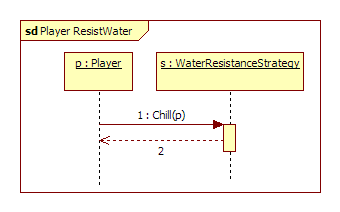
\includegraphics[width=10cm]{chapters/chapter03/seqdiag/Player_ResistWater.png}
		\caption{Player.ResistWater()}
		\label{fig:PlayerResistWater}
	\end{center}
\end{figure}
\begin{figure}[H]
	\begin{center}
		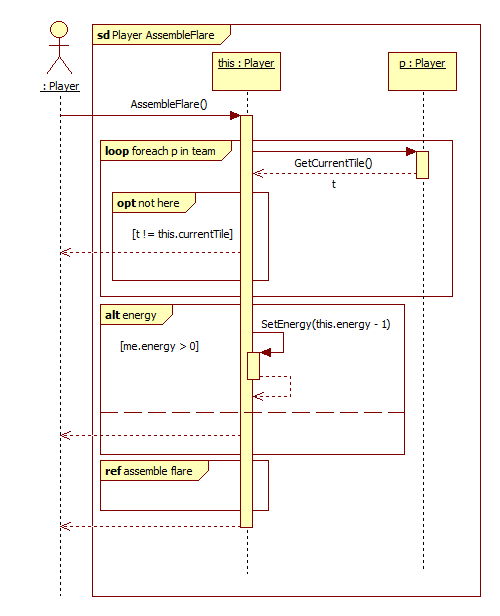
\includegraphics[width=10cm]{chapters/chapter03/seqdiag/Player_AssembleFlare.png}
		\caption{Player.AssembleFlare()}
		\label{fig:PlayerAssembleFlare}
	\end{center}
\end{figure}
\begin{figure}[H]
	\begin{center}
		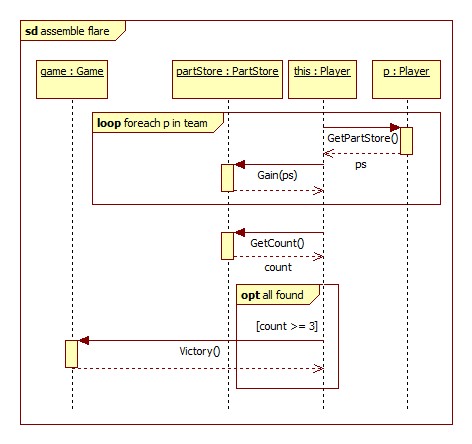
\includegraphics[width=10cm]{chapters/chapter03/seqdiag/Player_assemble_flare.png}
		\caption{Player.AssembleFlare()}
		\label{fig:PlayerAssembleFlare2}
	\end{center}
\end{figure}
\begin{figure}[H]
	\begin{center}
		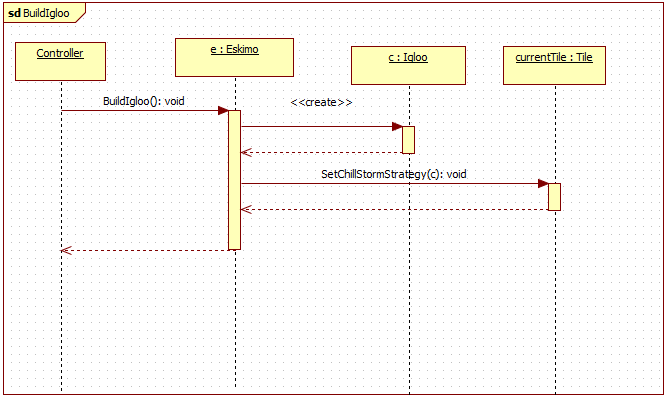
\includegraphics[width=15cm]{chapters/chapter03/seqdiag/Eskimo_BuildIgloo.png}
		\caption{Eskimo.BuildIgloo()}
		\label{fig:EskimoBuildIgloo}
	\end{center}
\end{figure}
\begin{figure}[H]
	\begin{center}
		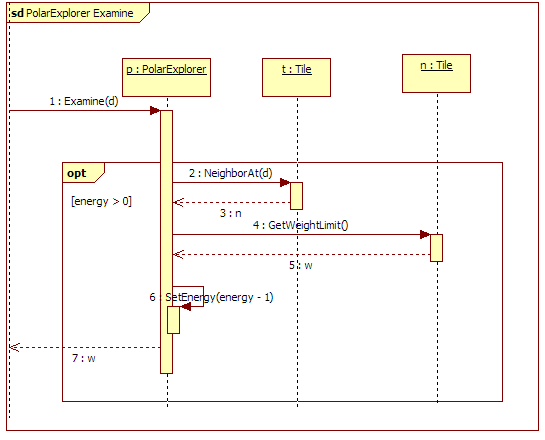
\includegraphics[width=15cm]{chapters/chapter03/seqdiag/PolarExplorer_Examine.png}
		\caption{PolarExplorer.Examine(direction: int)}
		\label{fig:PolarExplorerExamine}
	\end{center}
\end{figure}
\begin{figure}[H]
	\begin{center}
		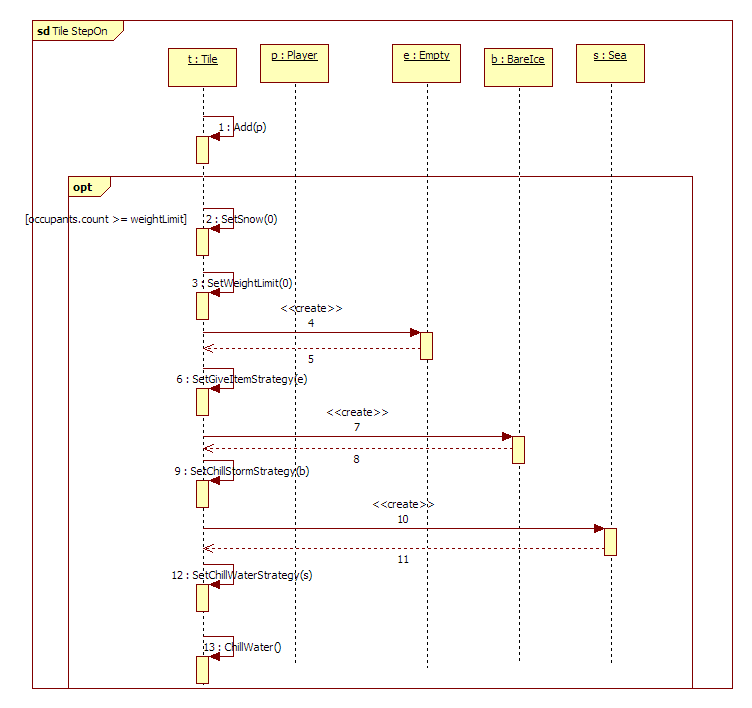
\includegraphics[width=15cm]{chapters/chapter03/seqdiag/Tile_StepOn.png}
		\caption{Tile.StepOn(Player)}
		\label{fig:TileStepOn}
	\end{center}
\end{figure}
\begin{figure}[H]
	\begin{center}
		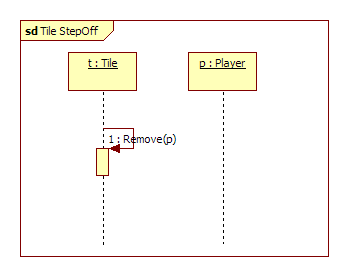
\includegraphics[width=10cm]{chapters/chapter03/seqdiag/Tile_StepOff.png}
		\caption{Tile.StepOff(Player)}
		\label{fig:TileStepOff}
	\end{center}
\end{figure}
\begin{figure}[H]
	\begin{center}
		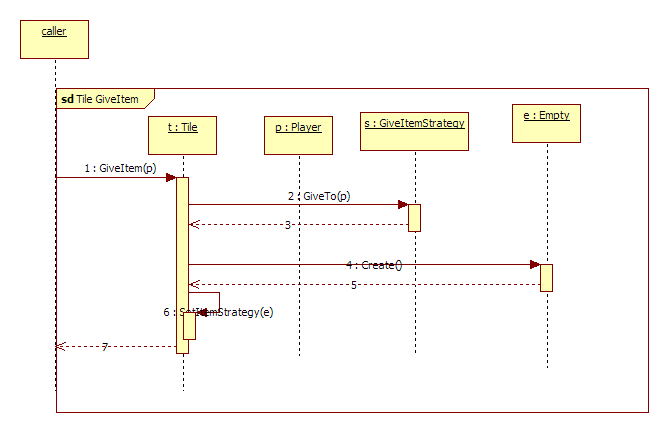
\includegraphics[width=14cm]{chapters/chapter03/seqdiag/Tile_GiveItem.png}
		\caption{Tile.GiveItem(Player)}
		\label{fig:TileGiveItem}
	\end{center}
\end{figure}
\begin{figure}[H]
	\begin{center}
		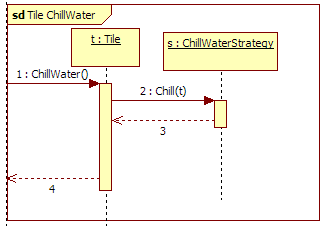
\includegraphics[width=10cm]{chapters/chapter03/seqdiag/Tile_ChillWater.png}
		\caption{Tile.ChillWater()}
		\label{fig:TileChillWater}
	\end{center}
\end{figure}
\begin{figure}[H]
	\begin{center}
		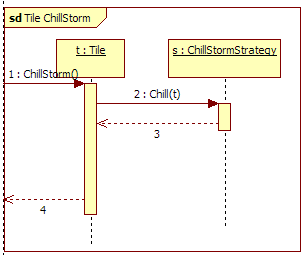
\includegraphics[width=10cm]{chapters/chapter03/seqdiag/Tile_ChillStorm.png}
		\caption{Tile.ChillStorm()}
		\label{fig:TileChillStorm}
	\end{center}
\end{figure}
\begin{figure}[H]
	\begin{center}
		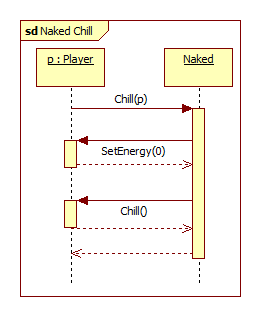
\includegraphics[width=10cm]{chapters/chapter03/seqdiag/Naked_Chill.png}
		\caption{Naked.Chill(Player)}
		\label{fig:NakedChill}
	\end{center}
\end{figure}
\begin{figure}[H]
	\begin{center}
		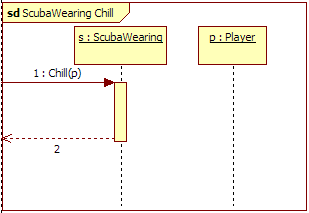
\includegraphics[width=10cm]{chapters/chapter03/seqdiag/ScubaWearing_Chill.png}
		\caption{ScubaWearing.Chill(Player)}
		\label{fig:ScubaWearingChill}
	\end{center}
\end{figure}
\begin{figure}[H]
	\begin{center}
		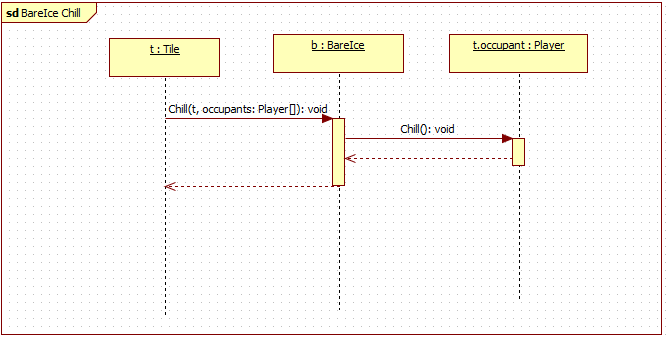
\includegraphics[width=15cm]{chapters/chapter03/seqdiag/BareIce_Chill.png}
		\caption{BareIce.Chill()}
		\label{fig:BareIceChill}
	\end{center}
\end{figure}
\begin{figure}[H]
	\begin{center}
		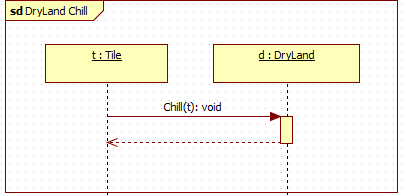
\includegraphics[width=10cm]{chapters/chapter03/seqdiag/DryLand_Chill.png}
		\caption{DryLand.Chill(Tile)}
		\label{fig:DryLandChill}
	\end{center}
\end{figure}
\begin{figure}[H]
	\begin{center}
		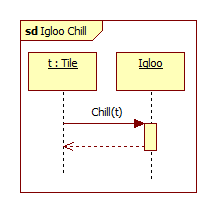
\includegraphics[width=10cm]{chapters/chapter03/seqdiag/Igloo_Chill.png}
		\caption{Igloo.Chill(Tile)}
		\label{fig:IglooChill}
	\end{center}
\end{figure}
\begin{figure}[H]
	\begin{center}
		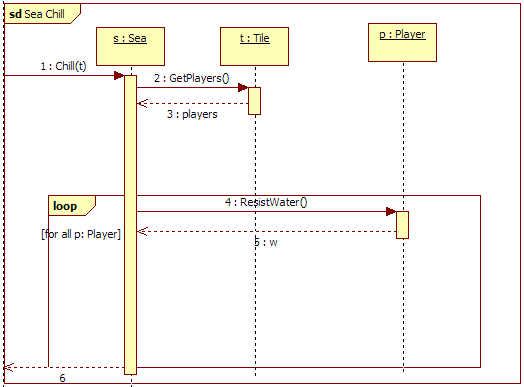
\includegraphics[width=13cm]{chapters/chapter03/seqdiag/Sea_Chill.png}
		\caption{Sea.Chill(Tile)}
		\label{fig:SeaChill}
	\end{center}
\end{figure}
\begin{figure}[H]
	\begin{center}
		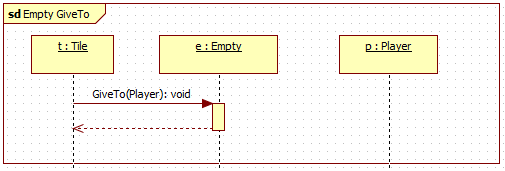
\includegraphics[width=13cm]{chapters/chapter03/seqdiag/Empty_GiveTo.png}
		\caption{Empty.GiveTo(Player)}
		\label{fig:EmptyGiveTo}
	\end{center}
\end{figure}
\begin{figure}[H]
	\begin{center}
		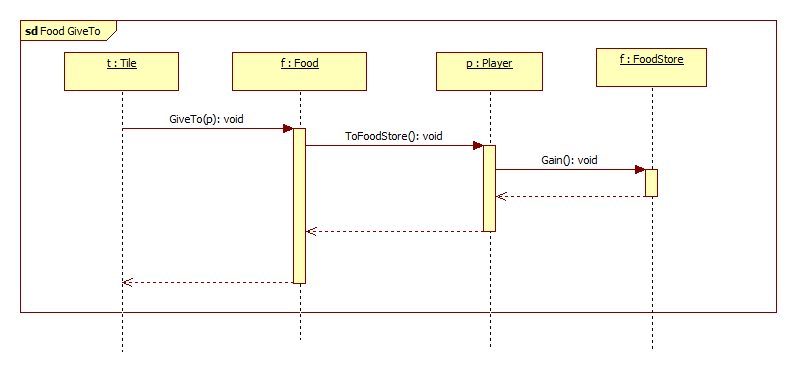
\includegraphics[width=15cm]{chapters/chapter03/seqdiag/Food_GiveTo.png}
		\caption{Food.GiveTo(Player)}
		\label{fig:FoodGiveTo}
	\end{center}
\end{figure}
\begin{figure}[H]
	\begin{center}
		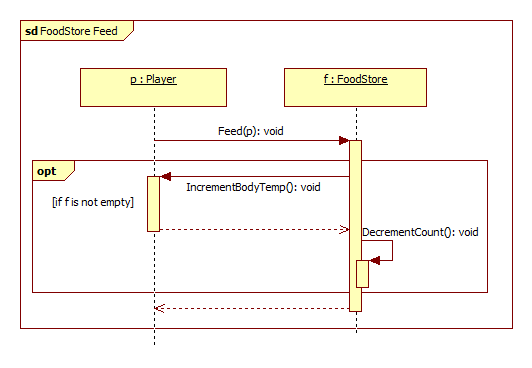
\includegraphics[width=12cm]{chapters/chapter03/seqdiag/FoodStore_Feed.png}
		\caption{FoodStore.Feed(Player)}
		\label{fig:FoodStoreFeed}
	\end{center}
\end{figure}
\begin{figure}[H]
	\begin{center}
		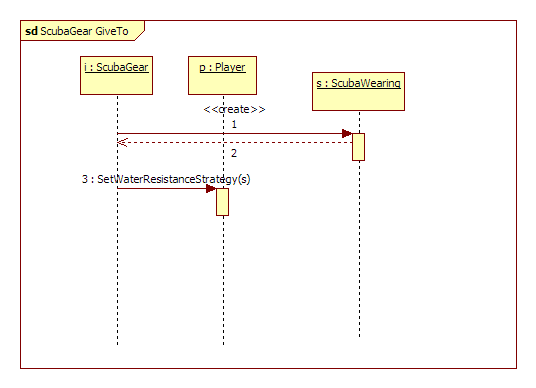
\includegraphics[width=10cm]{chapters/chapter03/seqdiag/ScubaGear_GiveTo.png}
		\caption{ScubaGear.GiveTo(Player)}
		\label{fig:ScubaGearGiveTo}
	\end{center}
\end{figure}
\begin{figure}[H]
	\begin{center}
		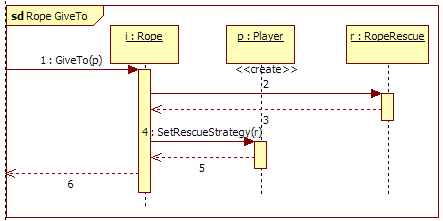
\includegraphics[width=10cm]{chapters/chapter03/seqdiag/Rope_GiveTo.png}
		\caption{Rope.GiveTo(Player)}
		\label{fig:RopeGiveTo}
	\end{center}
\end{figure}
\begin{figure}[H]
	\begin{center}
		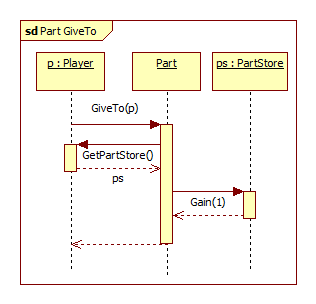
\includegraphics[width=10cm]{chapters/chapter03/seqdiag/Part_GiveTo.png}
		\caption{Part.GiveTo(Player)}
		\label{fig:PartGiveTo}
	\end{center}
\end{figure}
\begin{figure}[H]
	\begin{center}
		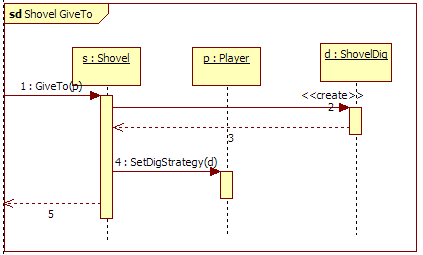
\includegraphics[width=10cm]{chapters/chapter03/seqdiag/Shovel_GiveTo.png}
		\caption{Shovel.GiveTo(Player)}
		\label{fig:ShovelGiveTo}
	\end{center}
\end{figure}
\begin{figure}[H]
	\begin{center}
		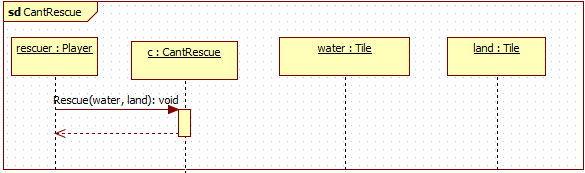
\includegraphics[width=13cm]{chapters/chapter03/seqdiag/CantRescue_Rescue.png}
		\caption{CantRescue.Rescue(Tile, Tile)}
		\label{fig:CantRescueRescue}
	\end{center}
\end{figure}
\begin{figure}[H]
	\begin{center}
		\includegraphics[width=13cm]{chapters/chapter03/seqdiag/RopeRescue_Rescue.png}
		\caption{RopeRescue.Rescue(Tile, Tile)}
		\label{fig:RopeRescueRescue}
	\end{center}
\end{figure}
\begin{figure}[H]
	\begin{center}
		\includegraphics[width=10cm]{chapters/chapter03/seqdiag/PartStore_Gain.png}
		\caption{PartStore.Gain(PartStore)}
		\label{fig:PartStoreGain}
	\end{center}
\end{figure}
\begin{figure}[H]
	\begin{center}
		\includegraphics[width=15cm]{chapters/chapter03/seqdiag/BareHandsDig_Dig.png}
		\caption{BareHandsDig.Dig(Tile)}
		\label{fig:BareHandsDig.Dig}
	\end{center}
\end{figure}
\begin{figure}[H]
	\begin{center}
		\includegraphics[width=10cm]{chapters/chapter03/seqdiag/ShovelDig_Dig.png}
		\caption{ShovelDig.Dig(Tile)}
		\label{fig:ShovelDigDig}
	\end{center}
\end{figure}




%\section{State-chartok}
%\comment{Csak azokhoz az osztályokhoz, ahol van értelme. Egyetlen állapotból álló state-chartok ne szerepeljenek. A játék működését bemutató state-chart-ot készíteni tilos.}
%\newpage
%\begin{figure}[h]
%\begin{center}
%\includegraphics[width=17cm]{chapters/chapter03/example.pdf}
%\caption{x}
%\label{fig:example3}
%\end{center}
%\end{figure}


% Szglab4
% ===========================================================================
%
\section{Napló}

\begin{naplo}

\bejegyzes{2020.03.05.~14:00~}{1 óra}{Kiss}{Ötletelés}
\bejegyzes{2020.03.07.~15:00~}{1 óra}{Glávits}{Ötletelés}
\bejegyzes{2020.03.07.~18:00~}{1 óra}{Kiss}{Glávits ötleteinek pontosítása}
\bejegyzes{2020.03.07.~19:00~}{1,5 óra}{Glávits}{Szekvenciák}
\bejegyzes{2020.03.07.~21:00~}{0,5 óra}{Glávits}{Dokumentáció}
\bejegyzes{2020.03.07.~23:00~}{1,5 óra}{Lant}{Class diagram update, javítás, Class diagram hibák keresése}
\bejegyzes{2020.03.08.~14:30~}{1 óra}{Kiss}{Dokumentáció javítgatás}

\end{naplo}


%
\setcounter{chapter}{4}
% Szglab4
% ===========================================================================
%
\chapter{Szkeleton tervezése}

\thispagestyle{fancy}

\section{A szkeleton modell valóságos use-case-ei}

\subsection{Use-case diagram}

\begin{figure}[h]
\begin{center}
\includegraphics[width=17cm]{chapters/chapter05/diagrams/TesztUseCase.jpg}
\caption{Use-case}
\label{fig:SzkeletonUseCase}
\end{center}
\end{figure}

\subsection{Use-case leírások}
% TODO: Valaki latexhez értő írja ezeket át itemize-ra, mert a latex jobbra húzza a bekezdés első sorát.
\usecase{Test PickUp Shovel}{Játékos lapátot vesz fel.}{Tester}{
	1. Eszkimó hóval nem rendelkező jégtáblán áll, amin egy lapát található.\newline
	2. Az eszkimó energiája csökken.\newline
	2.A Az eszkimó fáradt és nem tud tárgyat felvenni.\newline
	3. Az eszkimó felveszi a lapátot.\newline
	4. A lapát bekerül az eszkimó tárgyai közé és a megfelelő stratégiája helyére is.
}
\usecase{Test PickUp Food}{Játékos ételt vesz fel.}{Tester}{
	1. Eszkimó hóval nem rendelkező jégtáblán áll, amin egy élelem található.\newline
	2. Az eszkimó energiája csökken.\newline
	2.A Az eszkimó fáradt és nem tud tárgyat felvenni.\newline
	3. Az eszkimó felveszi az élelmet
	4. Az élelem bekerül az eszkimó tárgyai közé és a kajatárolójába is.
}
\usecase{Test PickUp Part}{Játékos alkatrészt vesz fel.}{Tester}{
	1. Eszkimó hóval nem rendelkező jégtáblán áll, amin egy rakéta alkatrész található.\newline
	2. Az eszkimó energiája csökken.\newline
	2.A Az eszkimó fáradt és nem tud tárgyat felvenni.\newline
	3. Az eszkimó felveszi az alkatrészt.\newline
	4. Az alkatrész bekerül az eszkimó tárgyai közé és a rakétadarabtárolójába is.
}
\usecase{Test PickUp Rope}{Játékos kötelet vesz fel.}{Tester}{
	1. Eszkimó hóval nem rendelkező jégtáblán áll, amin egy kötél található.\newline
	2. Az eszkimó energiája csökken.\newline
	2.A Az eszkimó fáradt és nem tud tárgyat felvenni.\newline
	3. Az eszkimó felveszi a kötelet.\newline
	4. A kötél bekerül az eszkimó tárgyai közé és a megfelelő stratégiája helyére is.
}
\usecase{Test PickUp ScubaGear}{Játékos búváruhát vesz fel.}{Tester}{
	1. Eszkimó hóval nem rendelkező jégtáblán áll, amin egy búvárruha található.\newline
	2. Az eszkimó energiája csökken.\newline
	2.A Az eszkimó fáradt és nem tud tárgyat felvenni.\newline
	3. Az eszkimó felveszi a búvárruhát.\newline
	4. A búvárruha bekerül az eszkimó tárgyai közé és a megfelelő stratégiája helyére is.
}
\usecase{Test BareHandsDig}{Játékos üres kézzel havat lapátol.}{Tester}{
	1. Eszkimó hóval rendelkező jégtáblán áll.\newline
	2. Az eszkimó energiája csökken.\newline
	2.A Az eszkimó fáradt és nem tud tárgyat felvenni.\newline
	3. Az eszkimó a lapátja segítségével 2 havat ellapátol a jégtábláról.
} 
\usecase{Test ShovelDig}{Játékos lapáttal havat lapátol.}{Tester}{
	1. Eszkimó hóval rendelkező jégtáblán áll.\newline
	2. Az eszkimó energiája csökken.\newline
	2.A Az eszkimó fáradt és nem tud tárgyat felvenni.\newline
	3. Az eszkimó a keze segítségével 1 havat ellapátol a jégtábláról.
} 
\usecase{Test StepOnIce}{Játékos jégre lép.}{Tester}{
	1. Eszkimó jégtáblán áll és van előtte egy másik jégtábla.\newline
	2. Az eszkimó energiája csökken.\newline
	2.A Az eszkimó fáradt és nem tud előrelépni.\newline
	3. Az eszkimó előrelép.
}
\usecase{Test StepOnUnstableIce WithScubaGear}{Búvárruhás játékos instabil jégre lép.}{Tester}{
	1. Búvárruhás eszkimó jégtáblán áll és van előtte egy másik jégtábla, ami csak egy főt bír el, és áll rajta egy másik eszkimó.\newline
	2. Az eszkimó energiája csökken.\newline
	2.A. Alter: Az eszkimó fáradt és nem tud előrelépni.\newline
	3. Az eszkimó előrelép.\newline
	4. A jégtábla beszakad.\newline
	5. A búvárruha megvédi az eszkimót a hideg víztől.
}
\usecase{Test StepOnUnstableIce Naked}{Játékos instabil jégre lép.}{Tester}{
	1. Eszkimó jégtáblán áll és van előtte egy másik jégtábla, ami csak egy főt bír el, és áll rajta egy másik eszkimó.\newline
	2. Az eszkimó energiája csökken.\newline
	2.A Az eszkimó fáradt és nem tud előrelépni.\newline
	3. Az eszkimó előrelép.\newline
	4. A jégtábla beszakad.\newline
	5. Az eszkimó elkezd fuldokolni a hideg vízben.
}
\usecase{Test StepInHole WithScubaGear}{Búvárruhás játékos lyukba esik.}{Tester}{
	1. Búvárruhás eszkimó jégtáblán áll és van előtte egy hóval fedett lyuk.\newline
	2. Az eszkimó energiája csökken.\newline
	2.A Az eszkimó fáradt és nem tud előrelépni.\newline
	3. Az eszkimó előrelép.\newline
	4. A hó beszakad.\newline
	5. A búvárruha megvédi az eszkimót a hideg víztől.
}
\usecase{Test StepInHole Naked}{Játékos lyukba esik.}{Tester}{
	1. Búvárruhás eszkimó jégtáblán áll és van előtte egy hóval fedett lyuk.\newline
	2. Az eszkimó energiája csökken.\newline
	2.A Az eszkimó fáradt és nem tud előrelépni.\newline
	3. Az eszkimó előrelép.\newline
	4. A hó beszakad.\newline
	5. Az eszkimó elkezd fuldokolni a hideg vízben.
}
\usecase{Test RopeRescue}{A játékos kiment egy másik, vízben fuldokló játékost.}{Tester}{
	1. A játékos egy jégtáblán áll, az előtte lévő tenger mezőn pedig egy másik fuldoklik.\newline
	2. A játékos kihúzza a vízből a fuldokló társát.\newline
	3. A játékos a saját mezőjére helyezi társát.
}
\usecase{Test EatFood}{A játékos elfogyaszt egy egység élelmet.}{Tester}{
	1. A játékos az élelem tárolójából elfogyaszt egy élelmet.\newline
	1.A A játékosnál nincs élelem, nem történik semmi.
}
\usecase{Test AssebleFlare}{A játékos összeszereli a jelzőrakétát.}{Tester}{
	1. A játékos egy mezőn áll, és megpróbálja összeszereli a jelzőrakétát.\newline
	1.A Ha van olyan másik játékos, aki nem ezen a mezőn áll, az összeszerelés sikertelen.\newline
	2. A játékos átveszi a mezőjén lévő többi játékostol az alkatrészeket.\newline
	2.A Ha nincs elég rakéta alkatrész a játékos(ok)nál, akkor az összeszerelés sikertelen.\newline
	3. A játékos összeszereli és elsüti a rakétát, ezzel megnyerve a játékot.
}
\usecase{Test BuildIgloo}{Eszkimó épít egy iglut.}{Tester}{
	1. Az eszkimó jégtáblán áll, és épít egy iglut.\newline
	1.A Az eszkimónak nincs energiája, nem tud iglut építeni.\newline
	1.B Az eszkimó megépíti az iglut, energiája csökken eggyel.
}
\usecase{Test ExamineTile}{Felfedező megvizsgálja az egyik szomszédos mezőt.}{Tester}{
	1. A felfedező megvizsgálja a szomszédos mezőt.\newline
	1.A A felfedezőnek nincs elég energiája, nem tudja megvizsgálni a mezőt.\newline
	1.B A felfedező megvizsgálta a mezőt, energiája csökken eggyel.
}
\usecase{Test Test Turn OnStableIce}{Játékos elkezdi a körét sima jégen.}{Tester}{
	1. Eszkimó jégtáblán áll, amikor elkezdődik a kör. \newline
	2. Az eszkimó energiája feltöltődik.
}
\usecase{Test Test Turn InWater WithScubaGear}{Játékos elkezdi a körét vízen búvárruhában.}{Tester}{
	1. Eszkimó búvárruhában vízben áll, amikor elkezdődik a kör. \newline
	2. Az eszkimó energiája feltöltődik. \newline
}
\usecase{Test Test Turn InWater Naked}{Játékos elkezdi a körét vízen búvárruha nélkül.}{Tester}{
	1. Eszkimó vízben fulladozik, amikor elkezdődik a kör. \newline
	2. Az eszkimó testhője fogy. \newline
	2.A Az eszkimó teljesen belefagyott a vízbe, nincs több testhője, a játék véget ér.
}
\usecase{Test ChillStorm Igloo }{Játékost igluban éri a hóvihar.}{Tester}{
	1. Eszkimó egy jégtáblán áll, ahol már van iglu. \newline
	2. Jön a hóvihar, de az eszkimót ez nem érdekli, ő nem fázik. \newline
}
\usecase{Test ChillStorm BareIce}{Játékost iglu nélküli jégen éri a hóvihar}{Tester}{
	1. Eszkimó egy jégtáblán áll, ahol nincs iglu. \newline
	2. Jön a hóvihar, és a szegény eszkimó fázik, a testhőjéből veszít. \newline
	2.A Jön a hóvihar, viszont az eszkimó teljesen megfagyott, nincs több testhője, a játék véget ér. \newline
}

\section{A szkeleton kezelői felületének terve, dialógusok}

A szkeleton program működésének ellenőrzéséhez egy saját osztályt fogunk létrehozni. A szkeleton program szöveges formátumban fogja megjeleníteni a függvény hívásokat és visszatérési értéküket, ezzel a szekvenciadiagrammokkal való egyezés majd könnyen ellenőrizhető lesz. Induláskor majd egy menü segítségével lehet választani a különböző szekvenciák közül. A menüt a konzolos ablakban a billentyűzet segítségével lehet majd vezérelni. A menüpontok amiből választani lehet így néz ki:
\begin{Verbatim}[samepage=true]
1. játékos
	1. tárgyat vesz fel
		1. lapát
		2. kötél
		3. alkatrész
		...
	2. havat lapátol
		1. lapáttal
		2. üres kézzel
		...
\end{Verbatim}
A szkeleton programban az objektumok csak asszociációkat tárolnak, egyéb állapotokat a felhasználótól kér majd be. Ezeket szintén a menüvezérelt módszerrel teszi. Kiválasztva egy esetet a teljes szekvencia lefutása automatikus, a kimenet következő képpen néz majd ki a konzolban:
\begin{Verbatim}[samepage=true]
myLoggerTest.DoTest() {
    myLoggerTest.fn1() {
        myDummyObject.DummyObject() {
        }
        myLoggerTest.fn2(myDummyObject, 10) {
            myDummyObject.fn3(20) {
            }
            return 1234;
        }
        return myDummyObject;
    }
}
\end{Verbatim}
A bejegyzésben objektum név . függvénynév (paraméterek) \{ ... \} formátumban jelenek meg a függvényhívások. A visszatérési értéket pedig a return után írja ki.

\pagebreak
\section{Szekvencia diagramok a belső működésre}

\begin{figure}[H]
	\begin{center}
		\includegraphics[width=17cm]{chapters/chapter05/diagrams/TestPickUpShovel.jpg}
		\caption{Test PickUp Shovel}
		\label{fig:Test PickUp Shovel}
	\end{center}
\end{figure}

\begin{figure}[H]
	\begin{center}
		\includegraphics[width=17cm]{chapters/chapter05/diagrams/TestPickUpFood.jpg}
		\caption{Test PickUp Food}
		\label{fig:Test PickUp Food}
	\end{center}
\end{figure}

\begin{figure}[H]
	\begin{center}
		\includegraphics[width=17cm]{chapters/chapter05/diagrams/TestPickUpPart.jpg}
		\caption{Test PickUp Part}
		\label{fig:Test PickUp Part}
	\end{center}
\end{figure}

\begin{figure}[H]
	\begin{center}
		\includegraphics[width=17cm]{chapters/chapter05/diagrams/TestPickUpRope.jpg}
		\caption{Test PickUp Rope}
		\label{fig:Test PickUp Rope}
	\end{center}
\end{figure}

\begin{figure}[H]
	\begin{center}
		\includegraphics[width=17cm]{chapters/chapter05/diagrams/TestPickUpScubaGear.jpg}
		\caption{Test PickUp ScubaGear}
		\label{fig:Test PickUp ScubaGear}
	\end{center}
\end{figure}

\begin{figure}[H]
	\begin{center}
		\includegraphics[width=15cm]{chapters/chapter05/diagrams/TestBareHandsDig.jpg}
		\caption{Test BareHandsDig}
		\label{fig:Test BareHandsDig}
	\end{center}
\end{figure}

\begin{figure}[H]
	\begin{center}
		\includegraphics[width=17cm]{chapters/chapter05/diagrams/TestShovelDig.jpg}
		\caption{Test ShovelDig}
		\label{fig:Test ShovelDig}
	\end{center}
\end{figure}

\begin{figure}[H]
	\begin{center}
		\includegraphics[width=13cm]{chapters/chapter05/diagrams/Test_StepOnIce.png}
		\caption{Test StepOnIce}
		\label{fig:Test StepOnIce}
	\end{center}
\end{figure}

\begin{figure}[H]
	\begin{center}
		\includegraphics[width=17cm]{chapters/chapter05/diagrams/Test_StepOnUnstableIce_WithScubaGear.png}
		\caption{Test StepOnUnstableIce WithScubaGear}
		\label{fig:Test StepOnUnstableIce WithScubaGear}
	\end{center}
\end{figure}

\begin{figure}[H]
	\begin{center}
		\includegraphics[width=17cm]{chapters/chapter05/diagrams/Test_StepOnUnstableIce_Naked.png}
		\caption{Test StepOnUnstableIce Naked}
		\label{fig:Test StepOnUnstableIce Naked}
	\end{center}
\end{figure}

\begin{figure}[H]
	\begin{center}
		\includegraphics[width=17cm]{chapters/chapter05/diagrams/Test_StepInHole_WithScubaGear.png}
		\caption{Test StepInHole WithScubaGear}
		\label{fig:Test StepInHole WithScubaGear}
	\end{center}
\end{figure}

\begin{figure}[H]
	\begin{center}
		\includegraphics[width=17cm]{chapters/chapter05/diagrams/Test_StepInHole_Naked.png}
		\caption{Test StepInHole Naked}
		\label{fig:Test StepInHole Naked}
	\end{center}
\end{figure}

\begin{figure}[H]
	\begin{center}
		\includegraphics[width=17cm]{chapters/chapter05/diagrams/Test_RopeRescue.jpg}
		\caption{Test RopeRescue}
		\label{fig:Test RopeRescue}
	\end{center}
\end{figure}

\begin{figure}[H]
	\begin{center}
		\includegraphics[width=12cm]{chapters/chapter05/diagrams/Test_EatFood.jpg}
		\caption{Test EatFood}
		\label{fig:Test EatFood}
	\end{center}
\end{figure}
\begin{figure}[H]
	\begin{center}
		\includegraphics[width=17cm]{chapters/chapter05/diagrams/Test_AssembleFlare.jpg}
		\caption{Test AssembleFlare}
		\label{fig:Test AssembleFlare}
	\end{center}
\end{figure}

\begin{figure}[H]
	\begin{center}
		\includegraphics[width=15cm]{chapters/chapter05/diagrams/Test_BuildIgloo.jpg}
		\caption{Test BuildIgloo}
		\label{fig:Test BuildIgloo}
	\end{center}
\end{figure}

\begin{figure}[H]
	\begin{center}
		\includegraphics[width=17cm]{chapters/chapter05/diagrams/Test_ExamineTile.jpg}
		\caption{Test ExamineTile}
		\label{fig:Test ExamineTile}
	\end{center}
\end{figure}

\begin{figure}[H]
	\begin{center}
		\includegraphics[width=17cm]{chapters/chapter05/diagrams/Test_Turn_OnStableIce.jpg}
		\caption{Test Turn OnStableIce}
		\label{fig:Test Turn OnStableIce}
	\end{center}
\end{figure}

\begin{figure}[H]
	\begin{center}
		\includegraphics[width=17cm]{chapters/chapter05/diagrams/Test_Turn_InWater_Naked.jpg}
		\caption{Test Turn InWater Naked}
		\label{fig:Test Turn InWater Naked}
	\end{center}
\end{figure}

\begin{figure}[H]
	\begin{center}
		\includegraphics[width=17cm]{chapters/chapter05/diagrams/Test_Turn_InWater_WithScubaGear.jpg}
		\caption{Test Turn InWater WithScubaGear}
		\label{fig:Test Turn InWater WithScubaGear}
	\end{center}
\end{figure}

\begin{figure}[H]
	\begin{center}
		\includegraphics[width=13cm]{chapters/chapter05/diagrams/Test_ChillStorm_Igloo.jpg}
		\caption{Test ChillStorm Igloo}
		\label{fig:Test ChillStorm Igloo}
	\end{center}
\end{figure}

\begin{figure}[H]
	\begin{center}
		\includegraphics[width=17cm]{chapters/chapter05/diagrams/Test_ChillStorm_BareIce.jpg}
		\caption{Test ChillStorm BareIce}
		\label{fig:Test ChillStorm BareIce}
	\end{center}
\end{figure}


\pagebreak
\section{Kommunikációs diagramok}

\begin{figure}[H]
	\begin{center}
		\includegraphics[width=17cm]{chapters/chapter05/diagrams/TestPickUpShovelInit.jpg}
		\caption{Test PickUp Shovel}
		\label{fig:Test PickUp Shovel}
	\end{center}
\end{figure}

\begin{figure}[H]
	\begin{center}
		\includegraphics[width=17cm]{chapters/chapter05/diagrams/TestPickUpFoodInit.jpg}
		\caption{Test PickUp Food}
		\label{fig:Test PickUp Food}
	\end{center}
\end{figure}

\begin{figure}[H]
	\begin{center}
		\includegraphics[width=17cm]{chapters/chapter05/diagrams/TestPickUpPartInit.jpg}
		\caption{Test PickUp Part}
		\label{fig:Test PickUp Part}
	\end{center}
\end{figure}

\begin{figure}[H]
	\begin{center}
		\includegraphics[width=17cm]{chapters/chapter05/diagrams/TestPickUpRopeInit.jpg}
		\caption{Test PickUp Rope}
		\label{fig:Test PickUp Rope}
	\end{center}
\end{figure}

\begin{figure}[H]
	\begin{center}
		\includegraphics[width=17cm]{chapters/chapter05/diagrams/TestPickUpScubaGearInit.jpg}
		\caption{Test PickUp ScubaGear}
		\label{fig:Test PickUp ScubaGear}
	\end{center}
\end{figure}

\begin{figure}[H]
	\begin{center}
		\includegraphics[width=17cm]{chapters/chapter05/diagrams/TestBareHandsDigInit.jpg}
		\caption{Test BareHandsDig}
		\label{fig:Test BareHandsDig}
	\end{center}
\end{figure}

\begin{figure}[H]
	\begin{center}
		\includegraphics[width=17cm]{chapters/chapter05/diagrams/TestShovelDigInit.jpg}
		\caption{Test ShovelDig}
		\label{fig:Test ShovelDig}
	\end{center}
\end{figure}

\begin{figure}[H]
	\begin{center}
		\includegraphics[width=11cm]{chapters/chapter05/diagrams/Test_StepOnIce_init.png}
		\caption{Test StepOnIce}
		\label{fig:Test StepOnIce}
	\end{center}
\end{figure}

\begin{figure}[H]
	\begin{center}
		\includegraphics[width=17cm]{chapters/chapter05/diagrams/Test_StepOnUnstableIce_WithScubaGear_init.png}
		\caption{Test StepOnUnstableIce WithScubaGear}
		\label{fig:Test StepOnUnstableIce WithScubaGear}
	\end{center}
\end{figure}

\begin{figure}[H]
	\begin{center}
		\includegraphics[width=17cm]{chapters/chapter05/diagrams/Test_StepOnUnstableIce_Naked_init.png}
		\caption{Test StepOnUnstableIce Naked}
		\label{fig:Test StepOnUnstableIce Naked}
	\end{center}
\end{figure}

\begin{figure}[H]
	\begin{center}
		\includegraphics[width=11cm]{chapters/chapter05/diagrams/Test_StepInHole_WithScubaGear_init.png}
		\caption{Test StepInHole WithScubaGear}
		\label{fig:Test StepInHole WithScubaGear}
	\end{center}
\end{figure}

\begin{figure}[H]
	\begin{center}
		\includegraphics[width=11cm]{chapters/chapter05/diagrams/Test_StepInHole_Naked_init.png}
		\caption{Test StepInHole Naked}
		\label{fig:Test StepInHole Naked}
	\end{center}
\end{figure}

\begin{figure}[H]
	\begin{center}
		\includegraphics[width=17cm]{chapters/chapter05/diagrams/Test_RopeRescue_init.jpg}
		\caption{Test RopeRescue}
		\label{fig:Test RopeRescue}
	\end{center}
\end{figure}

\begin{figure}[H]
	\begin{center}
		\includegraphics[width=17cm]{chapters/chapter05/diagrams/Test_EatFood_init.jpg}
		\caption{Test EatFood}
		\label{fig:Test EatFood}
	\end{center}
\end{figure}
\begin{figure}[H]
	\begin{center}
		\includegraphics[width=17cm]{chapters/chapter05/diagrams/Test_AssembleFlare_init.jpg}
		\caption{Test AssembleFlare}
		\label{fig:Test AssembleFlare}
	\end{center}
\end{figure}

\begin{figure}[H]
	\begin{center}
		\includegraphics[width=17cm]{chapters/chapter05/diagrams/Test_BuildIgloo_init.jpg}
		\caption{Test BuildIgloo}
		\label{fig:Test BuildIgloo}
	\end{center}
\end{figure}

\begin{figure}[H]
	\begin{center}
		\includegraphics[width=17cm]{chapters/chapter05/diagrams/Test_ExamineTile_init.jpg}
		\caption{Test ExamineTile}
		\label{fig:Test ExamineTile}
	\end{center}
\end{figure}

\begin{figure}[H]
	\begin{center}
		\includegraphics[width=17cm]{chapters/chapter05/diagrams/Test_Turn_OnStableIce_init.jpg}
		\caption{Test Turn OnStableIce}
		\label{fig:Test Turn OnStableIce}
	\end{center}
\end{figure}

\begin{figure}[H]
	\begin{center}
		\includegraphics[width=12cm]{chapters/chapter05/diagrams/Test_Turn_InWater_Naked_init.jpg}
		\caption{Test Turn InWater Naked}
		\label{fig:Test Turn InWater Naked}
	\end{center}
\end{figure}

\begin{figure}[H]
	\begin{center}
		\includegraphics[width=17cm]{chapters/chapter05/diagrams/Test_Turn_InWater_WithScubaGear_init.jpg}
		\caption{Test Turn InWater WithScubaGear}
		\label{fig:Test Turn InWater WithScubaGear}
	\end{center}
\end{figure}

\begin{figure}[H]
	\begin{center}
		\includegraphics[width=14cm]{chapters/chapter05/diagrams/Test_ChillStorm_Igloo_init.jpg}
		\caption{Test ChillStorm Igloo}
		\label{fig:Test ChillStorm Igloo}
	\end{center}
\end{figure}

\begin{figure}[H]
	\begin{center}
		\includegraphics[width=17cm]{chapters/chapter05/diagrams/Test_ChillStorm_BareIce_init.jpg}
		\caption{Test ChillStorm BareIce}
		\label{fig:Test ChillStorm BareIce}
	\end{center}
\end{figure}

\section{Napló}

\begin{naplo}

\bejegyzes{2020.03.15.~18:00~}{1 óra}{Kiss}{Feladatok kiadása a csapattagoknak}
\bejegyzes{2020.03.20.~19:00~}{4 óra}{Glávits}{Szekvencia rajzolás}
\bejegyzes{2020.03.20.~22.00~}{20 perc}{Lant}{Skeleton fv implementálás}
\bejegyzes{2020.03.21.~00:00~}{1 óra}{Glávits}{Logger implementálása}
\bejegyzes{2020.03.21.~10:00~}{1 óra}{Kiss}{Szekvencia rajzolás}
\bejegyzes{2020.03.21.~11:00~}{2 óra}{Kiss}{Kommunikációs diagram rajzolás}
\bejegyzes{2020.03.21.~11:00~}{1 óra}{Kiss}{Use-case diagram rajzolás}
\bejegyzes{2020.03.22.~13:00~}{1 óra}{Glávits}{Use-case forgatókönyvek}
\bejegyzes{2020.03.22.~13:00~}{15 perc}{Kiss}{Use-case forgatókönyvek}
\bejegyzes{2020.03.22.~18:45~}{1 óra}{Lant}{5.2 megírása, +fancyvbr}
\bejegyzes{2020.03.22.~21:30~}{2.5 óra}{Konrád}{Szekvencia és kommunikációs diagram rajzolás}


\end{naplo}


%
\setcounter{chapter}{5}
\chapter{Szkeleton beadás}

\thispagestyle{fancy}

\section{Fordítási és futtatási útmutató}
%\comment{A feltöltött program fordításával és futtatásával kapcsolatos útmutatás. Ennek tartalmaznia kell leltárszerűen az egyes fájlok pontos nevét, méretét byte-ban, keletkezési idejét, valamint azt, hogy a fájlban mi került megvalósításra.}

\subsection{Fájllista}

\begin{fajllista}

%\fajl{név}{méret}{keletkezés ideje}{leírás}
\fajl{build.bat}{0,53KB}{2020.03.28.~14:17~}{Fordító script}
\fajl{Logger.java}{4,44KB}{2020.03.20.~23:54~}{Naplózó osztály forráskódja}
\fajl{Main.java}{14,96KB}{2020.03.15.~18:33~}{A konzolalkalmazás belépési pontja}
\fajl{BareHands.java}{0,77KB}{2020.03.15.~18:33~}{... osztály forráskódja}
\fajl{BareIce.java}{0,67KB}{2020.03.15.~18:33~}{... osztály forráskódja}
\fajl{CantRescue.java}{0,73KB}{2020.03.15.~18:33~}{... osztály forráskódja}
\fajl{ChillStormStrategy.java}{0,28KB}{2020.03.15.~18:33~}{... osztály forráskódja}
\fajl{ChillWaterStrategy.java}{0,3KB}{2020.03.15.~18:33~}{... osztály forráskódja}
\fajl{DigStrategy.java}{0,27KB}{2020.03.15.~18:33~}{... osztály forráskódja}
\fajl{Direction.java}{0,53KB}{2020.03.28.~20:51~}{... osztály forráskódja}
\fajl{DryLand.java}{0,56KB}{2020.03.15.~18:33~}{... osztály forráskódja}
\fajl{Empty.java}{0,37KB}{2020.03.15.~18:33~}{... osztály forráskódja}
\fajl{Eskimo.java}{0,51KB}{2020.03.15.~18:33~}{... osztály forráskódja}
\fajl{Food.java}{0,43KB}{2020.03.15.~18:33~}{... osztály forráskódja}
\fajl{FoodStore.java}{0,92KB}{2020.03.15.~18:33~}{... osztály forráskódja}
\fajl{Game.java}{7,51KB}{2020.03.15.~18:33~}{... osztály forráskódja}
\fajl{Igloo.java}{0,44KB}{2020.03.15.~18:33~}{... osztály forráskódja}
\fajl{Item.java}{0,24KB}{2020.03.15.~18:33~}{... osztály forráskódja}
\fajl{Naked.java}{0,47KB}{2020.03.15.~18:33~}{... osztály forráskódja}
\fajl{Part.java}{0,46KB}{2020.03.15.~18:33~}{... osztály forráskódja}
\fajl{PartStore.java}{1,44KB}{2020.03.15.~18:33~}{... osztály forráskódja}
\fajl{Player.java}{11,18KB}{2020.03.15.~18:33~}{... osztály forráskódja}
\fajl{PolarExplorer.java}{0,68KB}{2020.03.15.~18:33~}{... osztály forráskódja}
\fajl{RescueStrategy.java}{0,42KB}{2020.03.15.~18:33~}{... osztály forráskódja}
\fajl{Rope.java}{0,51KB}{2020.03.15.~18:33~}{... osztály forráskódja}
\fajl{RopeRescue.java}{1,12KB}{2020.03.15.~18:33~}{... osztály forráskódja}
\fajl{ScubaGear.java}{0,56KB}{2020.03.15.~18:33~}{... osztály forráskódja}
\fajl{ScubaWearing.java}{0,53KB}{2020.03.15.~18:33~}{... osztály forráskódja}
\fajl{Sea.java}{0,59KB}{2020.03.15.~18:33~}{... osztály forráskódja}
\fajl{Shovel.java}{0,51KB}{2020.03.15.~18:33~}{... osztály forráskódja}
\fajl{ShovelDig.java}{1,13KB}{2020.03.15.~18:33~}{... osztály forráskódja}
\fajl{Tile.java}{4,81KB}{2020.03.15.~18:33~}{... osztály forráskódja}
\fajl{WaterResistanceStrategy.java}{0,38KB}{2020.03.15.~18:33~}{... osztály forráskódja}

\end{fajllista}

\subsection{Fordítás}
%\comment{A fenti listában szereplő forrásfájlokból milyen műveletekkel lehet a bináris, futtatható kódot előállítani. Az előállításhoz csak a 2. Követelmények c. dokumentumban leírt környezetet szabad előírni.}
A fordítást a skeleton\textbackslash{}build.bat script végzi. Létrehozza a skeleton\textbackslash{}out\textbackslash{}skeleton.jar fájlt, és el is indítja.

\subsection{Futtatás}
%\comment{A futtatható kód elindításával kapcsolatos teendők leírása. Az indításhoz csak a 2. Követelmények c. dokumentumban leírt környezetet szabad előírni.}

\lstset{escapeinside=`', xleftmargin=10pt, frame=single, basicstyle=\ttfamily\footnotesize, language=sh}
\begin{lstlisting}
java -jar skeleton\out\skeleton.jar
\end{lstlisting}

\section{Értékelés}
%\comment{A projekt kezdete óta az értékelésig eltelt időben tagokra bontva, százalékban.}

% !!!
% Hogyan fogjuk aláírni?
% !!!

\begin{ertekeles}
\tag{Kiss Andor} % Tag neve
{22}        % Munka szazalekban
\tag{Glávits Balázs Róbert}
{24}
\tag{Lant Gábor}
{18}
\tag{Konrád Márk}
{18}
\tag{Máté Botond}
{18}
\end{ertekeles}


\section{Napló}

\begin{naplo}

\bejegyzes{2020.03.28.~14:00~}{15 perc}{Glávits}{User prompt helper függvény megírása.}
\bejegyzes{2020.03.28.~15:00~}{1 óra}{Glávits}{Fordító script megírása.}
\bejegyzes{2020.03.28.~14.30~}{2,5 óra}{Lant}{Szekvencia ellenőrzések, kódolás}
\bejegyzes{2020.03.28.~18.30~}{1,5 óra}{Glávits}{Modell implementálás.}

\end{naplo}


%
\setcounter{chapter}{6}
% Szglab4
% ===========================================================================
%

\chapter{Prototípus koncepciója}

\thispagestyle{fancy}

\setcounter{section}{-1}

\section{Változás hatása a modellre}

\subsection{Módosult osztálydiagram}

\begin{figure}[H]
	\begin{center}
		%\includegraphics[angle=90, scale=0.76]{chapters/chapter07/ClassDiagramPart1.png}
		\includegraphics[width=18cm]{chapters/chapter07/ClassDiagramPart1.png}
		\caption{Osztálydiagram 1.}
		\label{fig:OsztalyDiagramPart1}
	\end{center}
\end{figure}
\begin{figure}[H]
	\begin{center}
		\includegraphics[width=17cm]{chapters/chapter07/ClassDiagramPart2.png}
		\caption{Osztálydiagram 2.}
		\label{fig:OsztalyDiagramPart2}
	\end{center}
\end{figure}

Új osztályok
\begin{itemize}
\item BreakingShovel
	\begin{itemize}
	\item implements Item
	\item Törékeny lapát tárgy.
	\end{itemize}
\item BreakingShovelDig
	\begin{itemize}
	\item implements DigStrategy
	\item Így ásnak a törékeny lapáttal.
	\end{itemize}
\item BuildStrategy
	\begin{itemize}
	\item A játékos így épít sátrat.
	\end{itemize}
\item Direction
	\begin{itemize}
	\item Egy irány a pálya négyzetrácson. Észak, dél, kelet, nyugat.
	\end{itemize}
\item Entity
	\begin{itemize}
	\item Egy dolog ami tud lépkedni a jégtáblákon.
	\item A játékosok és a jegesmedve, Entity-k.
	\end{itemize}
\item PolarBear
	\begin{itemize}
	\item implements Entity
	\item Megtámadja a játékosokat, akikkel találkozik.
	\end{itemize}
\item Shelter
	\begin{itemize}
	\item Egy jégtábla ilyen védelmet nyújt a rajta álló játékosoknak a medve és a vihar elől.
	\end{itemize}
\item Tent
	\begin{itemize}
	\item implements Shelter.
	\item Sátor.
	\end{itemize}
\item TentKit
	\begin{itemize}
	\item implements Item
	\item Ezzel a tárggyal lehet sátrat építeni.
	\end{itemize}
\end{itemize}

\subsection{Új vagy megváltozó metódusok}
%\comment{Az analízis modell osztályleírásaiból azon metódusok újbóli felsorolása leírással együtt, amelyek a változtatás miatt módosultak vagy újonnan be lettek vezetve.}
\begin{itemize}
\item Shelter.ChillStorm(Tile)
\begin{itemize} \item A paraméterként kapott Tilen lévő összes játékos fázik, meghívódik a Chill metódusuk. \end{itemize}

\item Shelter.BearAttack(Tile)
\begin{itemize} \item A paraméterként kapott Tilen lévő összes játékos elszenvedi a medvetámadást, meghívódik a BearAttack metódusuk.  \end{itemize}

\item Shelter.Break(Tile)
\begin{itemize} \item A metódus visszatér, nem csinál semmit, azért van, hogy leszármazottak felüldefiniálják. \end{itemize}

\item Igloo.ChillStorm()
\begin{itemize} \item A metódus visszatér, mert az igluban a játékosok nem fáznak. \end{itemize}

\item Igloo.BearAttack()
\begin{itemize} \item A metódus visszatér, mert az iglu véd a medvétől. \end{itemize}

\item Tile.ChillStorm()
\begin{itemize} \item A rajta lévő Shelter menedék ChillStorm metódusát hívja a hóviharban. \end{itemize}

\item Entity.Chill() 
\begin{itemize} \item A metódus visszatér, nem csinál semmit, azért van, hogy leszármazottak felüldefiniálják. \end{itemize}

\item Entity.ResistWater()
\begin{itemize} \item A metódus visszatér, nem csinál semmit, azért van, hogy leszármazottak felüldefiniálják. \end{itemize}

\item Entity.BearAttack()
\begin{itemize} \item A metódus visszatér, nem csinál semmit, azért van, hogy leszármazottak felüldefiniálják. \end{itemize}

\item Entitiy.Step(direction)
\begin{itemize} \item Az entitás lekéri a jelenlegi mezőjétől a mezőt, ami a paraméterként kapott irányban van, a jelenlegi mezőről lelép, átlép az újra. \end{itemize}

\item Entity.PlaceOn(t: Tile)
\begin{itemize} \item Az entitás a paraméterként kapott Tilere lép, beállítódik currentTile-jének az. \end{itemize}

\item Player.Step(direction)
\begin{itemize} \item A játékos energiája csökken, majd ősosztálya lépés metódusa hívódik, ugyanazt csinálja. \end{itemize}

\item Tile.BreakShelter()
\begin{itemize} \item A kör elején a jégtábla megpróbálja eltörni a rajta lévő menedéket, meghívva annak a Break metódusát. Nem minden menedék törik el, a Break metódus felüldefiniálásától függ ez végül. \end{itemize}

\item Tent.Break(t: Tile)
\begin{itemize} \item A sátor eltörik a kör elején, ezért a sátor halálát úgy jelzi, hogy a paraméterként kapott jégtábla(amin a sátor van) menedékét sima jégre beállítja. \end{itemize}

\item Tent.ChillStorm()
\begin{itemize} \item A metódus visszatér, mert a sátorban nem fázik az ember. \end{itemize}

\item TentKit.GiveTo(p: Player)
\begin{itemize} \item  A paraméterként kapott játékos kap a BuildStrategyjébe egy sátrat. p.BuildStrategy.IncrementCount() és kiveszi magát az inventoryból, mert consumable. \end{itemize}

\item BuildStrategy.Build(t:Tile)
\begin{itemize} \item  Eggyel fogy az építhető sátrak száma, majd a paraméterként kapott Tilere épül egy sátor. \end{itemize}

\item Player.Build()
\begin{itemize} \item A játékos energiája eggyel fogy, majd a megfelelő építési stratégiája függvényében épít a jelenlegi mezőjére. \end{itemize}

\item Eskimo.Build()
\begin{itemize} \item Az eszkimó energiája fogy eggyel, majd épít egy iglut a jelenlegi mezőjére. Nem érdekli őt, hogy van-e nála sátor, az iglu úgyis jobb. \end{itemize}

\item Game.initplayer
\begin{itemize} \item  A Game.CreateEskimo és a Game.CreatePolarExplorer közös részszekvenciája. A playernek ad egy BuildStrategyt, 0-ás számlálóval \end{itemize}

\item Game.Turn()
\begin{itemize} \item  A játékban új kör kezdődik, a játékosok energiája feltölt, ott meghívódik annak a metódusa, a vízben lévő  játékosok fáznak, a jégtáblákon lévő menedékek megpróbálnak eltörni. \end{itemize}

\item BreakingShovel.GiveTo(p: Player)
\begin{itemize} \item A paraméterként kapott Player megfelelő stratégiája helyére bekerül az eltörésre képes lapát, emellett az inventoryjába is. A lapát megjegyzi hány durabilityje van, és csak annyi ásást engedélyez a játékosnak eltörés előtt. \end{itemize}

\item BreakingShovelDig.Dig()
\begin{itemize} \item A lapát durabilityje csökken, minden második ásásra tér vissza igazzal, hogy egy energiával a játékos tudjon kettőt ásni. Ha a lapát eltört, a játékos mindenképp fárad, és nem ás ki havat a jégtábláról, egyébként igen. \end{itemize}

\item Game.CreatePolarBear()
\begin{itemize} \item A játék létrehoz egy jegesmaci objektumot, leteszi egy mezőre, hogy onnantól elinduljon véletlenszerű útján. \end{itemize}

\item PolarBear.Step(direction)
\begin{itemize} \item A paraméterként kapott irányba lép a jegesmaci, az ősosztálya lépéséhez hasonlóan, az ős lépés metódusa hívódik meg. A mezőt, amire rálépett, meg is támadja, hiszen falatozni akar az ízletes játékosok puha húsából. \end{itemize}

\item Player.BearAttack()
\begin{itemize} \item Ha egy játékost megtámadott a medve, nem tud védekezni ellene. Meghal, és a játék véget ér. \end{itemize}

\item Tile.BearAttack()
\begin{itemize} \item Az adott mezőt megtámadta a medve, ezért az szól a rajta lévő menedéknek, hogy megtámadta a medve, tegyen valamit. A menedék attól függően, hogy hogy definiálja felül a BearAttack(Tile) metódusát, védi meg, vagy hagyja meghalni az ott lévő játékosokat. \end{itemize}

\item Game.CreateTile(snow, weightLimit)
\begin{itemize} \item Ez a függvény a játék jégtáblagenerálásáért felel. A paraméterként kapott hó és teherbírásmennyiség függvénéyben generál jégtáblát, majd azt összekapcsolja szomszédaival. Ez a metódus majd a tesztelés során lesz nagyon hasznos. \end{itemize}

\end{itemize}


\subsection{Szekvencia-diagramok}

% TODO: labelezni, captionozni
% TODO: width-et állítani

\begin{figure}[H]
        \begin{center}
                \includegraphics[width=10cm]{chapters/chapter07/seqdiag/BreakingShovelDig_Dig.jpg}
                \caption{BreakingShovelDig Dig}
                \label{BreakingShovelDig Dig}
        \end{center}
\end{figure}
\begin{figure}[H]
        \begin{center}
                \includegraphics[width=10cm]{chapters/chapter07/seqdiag/BreakingShovel_GiveTo.png}
                \caption{BreakingShovel GiveTo}
                \label{BreakingShovel GiveTo}
        \end{center}
\end{figure}
\begin{figure}[H]
        \begin{center}
                \includegraphics[width=10cm]{chapters/chapter07/seqdiag/BuildStrategy_Build.jpg}
                \caption{BuildStrategy Build}
                \label{BuildStrategy Build}
        \end{center}
\end{figure}
\begin{figure}[H]
        \begin{center}
                \includegraphics[width=10cm]{chapters/chapter07/seqdiag/Entity_BearAttack.png}
                \caption{Entity BearAttack}
                \label{Entity BearAttack}
        \end{center}
\end{figure}
\begin{figure}[H]
        \begin{center}
                \includegraphics[width=10cm]{chapters/chapter07/seqdiag/Entity_Chill.jpg}
                \caption{Entity Chill}
                \label{Entity Chill}
        \end{center}
\end{figure}
\begin{figure}[H]
        \begin{center}
                \includegraphics[width=10cm]{chapters/chapter07/seqdiag/Entity_PlaceOn.png}
                \caption{Entity PlaceOn}
                \label{Entity PlaceOn}
        \end{center}
\end{figure}
\begin{figure}[H]
        \begin{center}
                \includegraphics[width=10cm]{chapters/chapter07/seqdiag/Entity_ResistWater.png}
                \caption{Entity ResistWater}
                \label{Entity ResistWater}
        \end{center}
\end{figure}
\begin{figure}[H]
        \begin{center}
                \includegraphics[width=10cm]{chapters/chapter07/seqdiag/Entity_Step.png}
                \caption{Entity Step}
                \label{Entity Step}
        \end{center}
\end{figure}
\begin{figure}[H]
        \begin{center}
                \includegraphics[width=10cm]{chapters/chapter07/seqdiag/Eskimo_Build.jpg}
                \caption{Eskimo Build}
                \label{Eskimo Build}
        \end{center}
\end{figure}
\begin{figure}[H]
        \begin{center}
                \includegraphics[width=10cm]{chapters/chapter07/seqdiag/Game_CreatePolarBear.jpg}
                \caption{Game CreatePolarBear}
                \label{Game CreatePolarBear}
        \end{center}
\end{figure}
\begin{figure}[H]
        \begin{center}
                \includegraphics[width=10cm]{chapters/chapter07/seqdiag/Game_CreateTile.png}
                \caption{Game CreateTile}
                \label{Game CreateTile}
        \end{center}
\end{figure}
\begin{figure}[H]
        \begin{center}
                \includegraphics[width=10cm]{chapters/chapter07/seqdiag/Game_init_player.png}
                \caption{Game init player}
                \label{Game init player}
        \end{center}
\end{figure}
\begin{figure}[H]
        \begin{center}
                \includegraphics[width=10cm]{chapters/chapter07/seqdiag/Game_Turn.png}
                \caption{Game Turn}
                \label{Game Turn}
        \end{center}
\end{figure}
\begin{figure}[H]
        \begin{center}
                \includegraphics[width=10cm]{chapters/chapter07/seqdiag/Igloo_BearAttack.jpg}
                \caption{Igloo BearAttack}
                \label{Igloo BearAttack}
        \end{center}
\end{figure}
\begin{figure}[H]
        \begin{center}
                \includegraphics[width=10cm]{chapters/chapter07/seqdiag/Igloo_ChillStorm.jpg}
                \caption{Igloo ChillStorm}
                \label{Igloo ChillStorm}
        \end{center}
\end{figure}
\begin{figure}[H]
        \begin{center}
                \includegraphics[width=10cm]{chapters/chapter07/seqdiag/Player_BearAttack.jpg}
                \caption{Player BearAttack}
                \label{Player BearAttack}
        \end{center}
\end{figure}
\begin{figure}[H]
        \begin{center}
                \includegraphics[width=10cm]{chapters/chapter07/seqdiag/Player_Build.jpg}
                \caption{Player Build}
                \label{Player Build}
        \end{center}
\end{figure}
\begin{figure}[H]
        \begin{center}
                \includegraphics[width=10cm]{chapters/chapter07/seqdiag/Player_Step.jpg}
                \caption{Player Step}
                \label{Player Step}
        \end{center}
\end{figure}
\begin{figure}[H]
        \begin{center}
                \includegraphics[width=10cm]{chapters/chapter07/seqdiag/PolarBear_Step.jpg}
                \caption{PolarBear Step}
                \label{PolarBear Step}
        \end{center}
\end{figure}
\begin{figure}[H]
        \begin{center}
                \includegraphics[width=10cm]{chapters/chapter07/seqdiag/RopeRescue_Rescue.jpg}
                \caption{RopeRescue Rescue}
                \label{RopeRescue Rescue}
        \end{center}
\end{figure}
\begin{figure}[H]
        \begin{center}
                \includegraphics[width=10cm]{chapters/chapter07/seqdiag/Sea_Chill.jpg}
                \caption{Sea Chill}
                \label{SeaChill}
        \end{center}
\end{figure}
\begin{figure}[H]
        \begin{center}
                \includegraphics[width=10cm]{chapters/chapter07/seqdiag/Shelter_BearAttack.jpg}
                \caption{Shelter BearAttack}
                \label{Shelter BearAttack}
        \end{center}
\end{figure}
\begin{figure}[H]
        \begin{center}
                \includegraphics[width=10cm]{chapters/chapter07/seqdiag/Shelter_Break.jpg}
                \caption{Shelter Break}
                \label{Shelter Break}
        \end{center}
\end{figure}
\begin{figure}[H]
        \begin{center}
                \includegraphics[width=10cm]{chapters/chapter07/seqdiag/Shelter_ChillStorm.jpg}
                \caption{Shelter ChillStorm}
                \label{Shelter ChillStorm}
        \end{center}
\end{figure}
\begin{figure}[H]
        \begin{center}
                \includegraphics[width=10cm]{chapters/chapter07/seqdiag/TentKit_GiveTo.jpg}
                \caption{TentKit GiveTo}
                \label{TentKit GiveTo}
        \end{center}
\end{figure}
\begin{figure}[H]
        \begin{center}
                \includegraphics[width=10cm]{chapters/chapter07/seqdiag/Tent_Break.jpg}
                \caption{Tent Break}
                \label{Tent Break}
        \end{center}
\end{figure}
\begin{figure}[H]
        \begin{center}
                \includegraphics[width=10cm]{chapters/chapter07/seqdiag/Tent_ChillStorm.jpg}
                \caption{Tent ChillStorm}
                \label{Tent ChillStorm}
        \end{center}
\end{figure}
\begin{figure}[H]
        \begin{center}
                \includegraphics[width=10cm]{chapters/chapter07/seqdiag/Tile_BearAttack.jpg}
                \caption{Tile BearAttack}
                \label{Tile BearAttack}
        \end{center}
\end{figure}
\begin{figure}[H]
        \begin{center}
                \includegraphics[width=10cm]{chapters/chapter07/seqdiag/Tile_BreakShelter.png}
                \caption{Tile BreakShelter}
                \label{Tile BreakShelter}
        \end{center}
\end{figure}
\begin{figure}[H]
        \begin{center}
                \includegraphics[width=10cm]{chapters/chapter07/seqdiag/Tile_ChillStorm.jpg}
                \caption{Tile ChillStorm}
                \label{Tile ChillStorm}
        \end{center}
\end{figure}
\begin{figure}[H]
        \begin{center}
                \includegraphics[width=10cm]{chapters/chapter07/seqdiag/Tile_StepOff.jpg}
                \caption{Tile StepOff}
                \label{Tile StepOff}
        \end{center}
\end{figure}
\begin{figure}[H]
        \begin{center}
                \includegraphics[width=10cm]{chapters/chapter07/seqdiag/Tile_StepOn.jpg}
                \caption{Tile StepOn}
                \label{Tile StepOn}
        \end{center}
\end{figure}

\section{Prototípus interface-definíciója}
%\comment{Definiálni kell a teszteket leíró nyelvet. Külön figyelmet kell fordítani arra, hogy ha a rendszer véletlen elemeket is tartalmaz, akkor a véletlenszerűség ki-bekapcsolható legyen, és a program determinisztikusan is tesztelhető legyen.}

\subsection{Az interfész általános leírása}
%\comment{A protó (karakteres) input és output felületeit úgy kell kialakítani, hogy az input fájlból is vehető legyen illetőleg az output fájlba menthető legyen, vagyis kommunikációra csak a szabványos be- és kimenet használható.}
A program egysoros parancsokat vár a standard bemeneten. A játék kezdőállapotát definíciós parancsokkal kell megadni, majd vezérő parancsokkal lehet játszani. A \texttt{query} speciális parancs hatására, a játék teljes jelenlegi állapota kiíródik a standard kimenetre, definíciós parancsok sorozataként.

\subsection{Bemeneti nyelv}
%\comment{Definiálni kell a teszteket leíró nyelvet. Külön figyelmet kell fordítani arra, hogy ha a rendszer véletlen elemeket is tartalmaz, akkor a véletlenszerűség ki-bekapcsolható legyen, és a program determinisztikusan is futtatható legyen. A szálkezelést is tesztelhető, irányítható módon kell megoldani.}

\definecolor{mymaroon}{rgb}{0.5, 0.07, 0}
\definecolor{myblue}{rgb}{0, 0.02, 0.9}
\lstset{
	breakatwhitespace=false,
	keepspaces=false,
	breaklines=true,
	frame=L,
	numbers=left,
	language=C, %kicsit hasonlít a C-re
	basicstyle=\small\ttfamily,
	identifierstyle=\color{myblue},
	stringstyle=\color{mymaroon},
	caption={A program által elfogadott bemeneti nyelvtan Extended Backus-Naur formában.},
	label=GrammarEBNF
}
\lstinputlisting{chapters/chapter07/grammar.ebnf}

Szótár:

\begin{itemize}
\item \texttt{action\textunderscore{}command}
A jelenleg kiválasztott játékos cselekvése.
\item \texttt{assemble\textunderscore{}command}
A jelenleg kiválasztott játékos összeszereli a rakétát.
\item \texttt{build\textunderscore{}command}
A jelenleg kiválasztott játékos iglut/sátrat épít.
\item \texttt{building\textunderscore{}command}
A jelenleg kiválasztott cellára iglu/sátor épül.
\item \texttt{building\textunderscore{}type}
Iglu vagy sátor.
\item \texttt{command\textunderscore{}end}
Parancsok közti karaktersorozat, amit nem értelmezünk.
\item \texttt{comment}
\# karaktertől a sor végéig lehet komment.
\item \texttt{connect\textunderscore{}command}
A jelenleg kiválasztott cella szomszédaihoz adja az adott cellá(ka)t.
\item \texttt{dig\textunderscore{}command}
A jelenleg kiválasztott játékos havat lapátol.
\item \texttt{entity\textunderscore{}command}
Egy entitás létrehozása.
\item \texttt{entity\textunderscore{}definition}
Egy entitás létrehozása és tulajdonságainak beállítása.
\item \texttt{equip\textunderscore{}all\textunderscore{}command}
A jelenleg kiválasztott játékos felveszi az összes birtokában lévő tárgyat.
\item \texttt{equip\textunderscore{}command}
A jelenleg kiválasztott játékos felvesz birtokában lévő tárgyat.
\item \texttt{equip\textunderscore{}index}
Egy - játékos által birtokolt - tárgy száma.
\item \texttt{equip\textunderscore{}index\textunderscore{}command}
A jelenleg kiválasztott játékos felveszi az adott birtokában lévő tárgyat.
\item \texttt{examine\textunderscore{}command}
A jelenleg kiválasztott sarkkutató játékos felderít egy cellát.
\item \texttt{game}
Parancsok helyes sorozata.
\item \texttt{integer}
Nemnegatív egész szám, tízes számrendszerben.
\item \texttt{item\textunderscore{}command}
Tárgy/Tárgyak létrehozása.
\item \texttt{item\textunderscore{}command\textunderscore{}multiple}
Több tárgy létrehozása.
\item \texttt{item\textunderscore{}command\textunderscore{}single}
Egy tárgy létrehozása.
\item \texttt{item\textunderscore{}count}
Tárgyak számának megadása.
\item \texttt{item\textunderscore{}durability}
A törékeny lapát tárgy hátramaradt használásainak száma.
\item \texttt{item\textunderscore{}type}
Tárgy megadása.
\item \texttt{map\textunderscore{}definition}
A pálya létrehozása.
\item \texttt{pickup\textunderscore{}command}
A jelenleg kiválasztott játékos kiás egy tárgyat a jégből.
\item \texttt{player\textunderscore{}actions}
Egy játékos cselekedetei.
\item \texttt{player\textunderscore{}bodyheat}
Egy játékos testhője.
\item \texttt{player\textunderscore{}class}
Játékos osztály megadása: eszkimó/sarkkutató.
\item \texttt{player\textunderscore{}command}
Egy játékos létrehozása.
\item \texttt{player\textunderscore{}definition}
Egy játékos létrehozása, és birtokolt tárgyainak beállítása.
\item \texttt{player\textunderscore{}energy}
Játékos hátramaradt energiája.
\item \texttt{player\textunderscore{}equipped\textunderscore{}items}
Ezeket a tárgyakat a játékos felveszi.
\item \texttt{player\textunderscore{}index}
Játékos száma.
\item \texttt{player\textunderscore{}inventory\textunderscore{}items}
Ezek a tárgyak a játékos birtokába kerülnek.
\item \texttt{polarbear\textunderscore{}actions}
A jelenleg kiválasztott jegesmedve cselekedetei.
\item \texttt{polarbear\textunderscore{}command}
A jelenleg kiválasztott jegesmedve létrehozása.
\item \texttt{polarbear\textunderscore{}index}
Jegesmedve száma.
\item \texttt{query\textunderscore{}command}
A parancs hatására \texttt{map\textunderscore{}definition} íródik ki az stdout-ra, ami reprezentálja a játék jelenlegi állapotát.
\item \texttt{rescue\textunderscore{}command}
A jelenleg kiválasztott játékos kíhúzza csapattársát a vízből.
\item \texttt{select\textunderscore{}tile\textunderscore{}command}
Kiválaszt egy cellát.
\item \texttt{select\textunderscore{}player\textunderscore{}command}
Kiválaszt egy játékost.
\item \texttt{select\textunderscore{}polarbear\textunderscore{}command}
Kiválaszt egy jegesmedvét.
\item \texttt{step\textunderscore{}command}
A jelenleg kiválasztott játékos lép.
\item \texttt{storm\textunderscore{}command}
Hóvihar kezdődik.
\item \texttt{tile\textunderscore{}command}
Egy cella létrehozása.
\item \texttt{tile\textunderscore{}definition}
Egy cella létrehozása, és a rajta lévő dolgok létrehozása.
\item \texttt{tile\textunderscore{}snow}
A cella hószintjének definiálása.
\item \texttt{tile\textunderscore{}topology}
A cella szomszédainak beállítása.
\item \texttt{tile\textunderscore{}weight\textunderscore{}limit}
A cella teherbírásának definiálása: hány entitás állhat rajta. \newline A * karakter végtelen teherbírást jelöl. A 0 teherbírású cella tenger.
\item \texttt{turn\textunderscore{}command}
A parancs hatására új kör kezdődik a játékban.
\item \texttt{turn\textunderscore{}definition}
Egy kör során végrehajtott parancsok sorozata.
\end{itemize}

%\comment{Ha szükséges, meg kell adni a konfigurációs (pl. pályaképet megadó) fájlok nyelvtanát is.}

\subsection{Kimeneti nyelv}
%\comment{Egyértelműen definiálni kell, hogy az egyes bemeneti parancsok végrehajtása után előálló állapot milyen formában jelenik meg a szabványos kimeneten.}
A kimeneti nyelv a bemeneti nyelv részhalmaza. Pontosabban, egy  \texttt{map\textunderscore{}definition} nyelvi elem. Kivételes esetek a következők:
\begin{itemize}
\item Sarkkutató felderít egy cellát.
	\begin{itemize}
	\item Az \texttt{examine\textunderscore{}command} lefutását követően üzenet jelenik meg a standard kimeneten: \newline \texttt{"Tile weight limit: N\textbackslash{}n"}, ahol N a cella teherbírása.
	\end{itemize}
\item Egy játékos meghal.
	\begin{itemize}
	\item Üzenet jelenik meg: \texttt{"Game over.\textbackslash{}n"}, és a program megáll.
	\end{itemize}
\item A játékosok összeszerelik a rakétát.
	\begin{itemize}
	\item Üzenet jelenik meg: \texttt{"Victory.\textbackslash{}n"}, és a program megáll.
	\end{itemize}
\end{itemize}

\section{Összes részletes use-case}
%\comment{A use-case-eknek a részletezettsége feleljen meg a kezelői felületnek, azaz a felület elemeire kell hivatkozniuk. Alábbi táblázat minden use-case-hez külön-külön.}

\begin{figure}[h]
\begin{center}
\includegraphics[width=17cm]{chapters/chapter07/ProtoUseCases.png}
\caption{Use-case diagram}
\label{fig:ProtoUseCases}
\end{center}
\end{figure}

% TODO
\newpage % ha ez nincs, akkor a diagram beketül a táblázatok közé
% de így is bugos, mert egy-két táblázat lecsúszik a lapról

%\usecase{grid}{Pályaméret beállítása.}{Proto}{
%	1. Jön egy \texttt{grid\textunderscore{}command}.\newline
%	2. A pályaméret beállítódik.
%}
\usecase{tile}{Cella létrehozása.}{Proto}{
	1. Jön egy \texttt{tile\textunderscore{}command}.\newline
	2. Létrejön az adott cella.
}
\usecase{building}{Épület létrehozása.}{Proto}{
	1. Jön egy \texttt{building\textunderscore{}command}.\newline
	2. Létrejön az adott épület.
}
\usecase{item}{Tárgy létrehozása.}{Proto}{
	1. Jön egy \texttt{item\textunderscore{}command}.\newline
	2. Létrejön az adott tárgy, vagy tárgyak.
}
\usecase{equip}{Tárgy felvétele.}{Proto}{
	1. Jön egy \texttt{equip\textunderscore{}command}.\newline
	2. A jelenleg kiválasztott játékos felvesz egy tárgyat.
}
\usecase{entity}{Entitás létrehozása.}{Proto}{
	1. Jön egy \texttt{entity\textunderscore{}command}.\newline
	2. Létrejön az adott entitás.
}
\usecase{select}{Entitás kiválasztása.}{Proto}{
	1. Jön egy \texttt{select\textunderscore{}command}.\newline
	2. Kiválasztódik az adott entitás
}
\usecase{turn}{Új kör kezdése.}{Proto}{
	1. Jön egy \texttt{turn\textunderscore{}command}.\newline
	2. Új kör kezdődik.
}
\usecase{storm}{Vihar kezdése.}{Proto}{
	1. Jön egy \texttt{storm\textunderscore{}command}.\newline
	2. Vihar kezdődik.
}
\usecase{step}{Entitás lép.}{Proto}{
	1. Jön egy \texttt{step\textunderscore{}command}.\newline
	2. A jelenleg kiválasztott entitás lép.
}
\usecase{rescue}{Játékos megment.}{Proto}{
	1. Jön egy \texttt{rescue\textunderscore{}command}.\newline
	2. A jelenleg kiválasztott játékos kíhúzza csapattársát a vízből.
}
\usecase{dig}{Játékos lapátol.}{Proto}{
	1. Jön egy \texttt{dig\textunderscore{}command}.\newline
	2. A jelenleg kiválasztott játékos lapátol.
}
\usecase{pickup}{Játékos felvesz.}{Proto}{
	1. Jön egy \texttt{pickup\textunderscore{}command}.\newline
	2. A jelenleg kiválasztott játékos kiás egy tárgyat.
}
\usecase{build}{Játékos épít.}{Proto}{
	1. Jön egy \texttt{build\textunderscore{}command}.\newline
	2. A jelenleg kiválasztott játékos épít.
}
\usecase{assemble}{Játékos összeszerel}{Proto}{
	1. Jön egy \texttt{assemble\textunderscore{}command}.\newline
	2. A jelenleg kiválasztott játékos összeszereli a rakétát.
}
\usecase{examine}{Jégtábla felderítése}{Proto}{
	1. Jön egy \texttt{examine\textunderscore{}command}.\newline
	2. A jelenleg kiválasztott sarkkutató játékos felderít egy mezőt.
}
\usecase{query}{A játékállapot lekérdezése.}{Proto}{
	1. Jön egy \texttt{query\textunderscore{}command}.\newline
	2. A játék állapota kiíródik a standard kimenetre.
}

\section{Tesztelési terv}
%\comment{A tesztelési tervben definiálni kell, hogy a be- és kimeneti fájlok egybevetésével miként végezhető el a program tesztelése. Meg kell adni teszt forgatókönyveket. Az egyes teszteket elég informálisan, szabad szövegként leírni. Teszt-esetenként egy-öt mondatban. Minden teszthez meg kell adni, hogy mi a célja, a proto mely funkcionalitását, osztályait stb. teszteli. Az alábbi táblázat minden teszt-esethez külön-külön elkészítendő.}

\teszteset{PickUpFood}{A játékos az adott mezőre lép. A mezőn élelem található. A játékos felveszi és a saját zsebébe rakja az ételt.}{Item felvétel teszt.}
\teszteset{PickUpPart}{A játékos adott mezőre lép. A mezőn rakéta pisztoly darab található. A játékos felveszi és a megfelelő zsebébe rakja.}{Item felvétel teszt.}
\teszteset{PickUpShovel}{A játékos adott mezőre lép. A mezőn ásó található. A játékos felvesz és a zsebébe rakja. A játékos ez utána már tud ásni később.}{Item felvétel teszt.}
\teszteset{PickUpBreakableShovel}{A játékos adott mezőre lép. A mezőn törékeny ásó található. A játékos felvesz és a zsebébe rakja. A játékos ez utána már tud ásni később.}{Item felvétel teszt.}
\teszteset{PickUpRope}{A játékos adott mezőre lép. A mezőn kötél található. A játékos felvesz és a zsebébe rakja. A játékos ez utána már ki tudja menteni a csapattársait.}{Item felvétel teszt.}
\teszteset{PickUpScubaGear}{A játékos adott mezőre lép. A mezőn búvárruha található. A játékos felvesz és a zsebébe rakja. A játékos ez utána már képes túlélni a vízben.}{Item felvétel teszt.}
\teszteset{PickUpTent}{A játékos adott mezőre lép. A mezőn sátor található. A játékos felvesz és a zsebébe rakja. A játékos ez utána már képes sátrat építeni egy mezőre.}{Item felvétel teszt.}
\teszteset{BareHandsDig}{A játékos azon a mezőn ahol éppen áll havat lapátol. A hómennyiség az adott mezőn csökken}{Hó lapátolás.}
\teszteset{ShovelDig}{A játékos azon a mezőn ahol éppen áll havat lapátol, van nála lapát. A hómennyiség az adott mezőn csökken}{Hó lapátolás.}
\teszteset{BreakingShovelDig}{A játékos azon a mezőn ahol éppen áll havat lapátol, van nála törékeny lapát. A hómennyiség az adott mezőn csökken. A lapát még nem törik el.}{Hó lapátolás.}
\teszteset{BreakingShovelDig}{A játékos azon a mezőn ahol éppen áll havat lapátol, van nála törékeny lapát. A hómennyiség az adott mezőn csökken. A lapát eltörik}{Hó lapátolás.}
\teszteset{StepOnStableIce}{A játékos stabil jégre lép.}{Játékos mezőre lép.}
\teszteset{StepOnUnstableIceWithScubaGearBreaking}{A játékos instabil jégre lép. A játékoson van búvárruha. A jég eltörik, mert nem bírja el. Minden játékos vízbe esik aki ott volt.}{Játékos mezőre lép.}
\teszteset{StepOnUnstableIceWithScubaGearCanHold}{A játékos instabil jégre lép. A játékoson van búvárruha. A jég nem törik el.}{Játékos mezőre lép.}
\teszteset{StepOnUnstableIceNakedBreaking}{A játékos instabil jégre lép. A játékoson nincs búvárruha. A jég eltörik, mert nem bírja el. Minden játékos vízbe esik aki ott volt.}{Játékos mezőre lép.}
\teszteset{StepOnUnstableIceNakedCanHold}{A játékos instabil jégre lép. A játékoson nincs búvárruha. A jég nem törik el.}{Játékos mezőre lép.}
\teszteset{StepInWaterWithScubaGear}{A játékos víz mezőre lép. A játékoson van búvárruha. A játékos kibírja a vízbe esést.}{Játékos mezőre lép.}
\teszteset{StepInWaterNaked}{A játékos víz mezőre lép. A játékoson nincs búvárruha.A játékos meg fog fagyni, ha nem mentik ki később.}{Játékos mezőre lép.}
\teszteset{RopeRescue}{A játékosnak van kötele. Egy játékos kiment egy másik játékost a vízből és a saját táblájára húzza.}{Játékos cselekszik}
\teszteset{EatFood}{A játékosnak van élelme. A játékos elfogyaszt 1 élelmet a zsebéből és nő a testhője.}{Játékos cselekszik.}
\teszteset{AssembleFlare}{A játékosnál van az összes rakéta darab. A játékos összeszereli azt.}{Játékos cselekszik.}
\teszteset{AssembleFlareFail}{A játékosnál nincs meg az összes rakéta darab és megpróbálja összeszerelni a pisztolyt.}{Játékos cselekszik.}
\teszteset{BuildIgloo}{Az eszkimó felvesz egy TentKit-et. Az eszkimó a táblára iglut épít, nem pedig sátrat.}{Tábla esemény teszt.}
\teszteset{BuildTent}{A sarkkutató felvesz egy TentKit-et. A sarkkutató a táblára sátrat épít.}{Tábla esemény teszt.}
\teszteset{ExamineTile}{A sarkkutató a táblát vizsgálja.}{Tábla esemény teszt.}
\teszteset{TurnOnStableIce}{Egy játék kör eltelik úgy, hogy a játékos a stabil jégen áll.}{Játék esemény teszt.}
\teszteset{TurnInWaterNaked}{Egy játék kör eltelik úgy, hogy a játékos vízben áll. A játékoson van búvárruha.}{Játék esemény teszt.}
\teszteset{TurnInWaterWithScubaGear}{Egy játék kör eltelik úgy, hogy a játékos vízben áll. A játékoson nincs búvárruha.}{Játék esemény teszt.}
\teszteset{ChillStormIgloo}{Egy játék kör eltelik, úgy, hogy a játékost hóvihar éri. A játékos igluban van.}{Játék esemény teszt.}
\teszteset{ChillStormTent}{Egy játék kör eltelik, úgy, hogy a játékost hóvihar éri. A játékos sátorban van.}{Játék esemény teszt.}
\teszteset{ChillStormBareIce}{Egy játék kör eltelik, úgy, hogy a játékost hóvihar éri. A játékos szabad ég alatt van.}{Játék esemény teszt.}
\teszteset{TentBreaking}{A táblán a sátor eltörik a kör után.}{Játék esemény teszt.}
\teszteset{PolarBearMoving}{A medve véletlen irányba lép. Üres mezőre lép.}{Játék esemény teszt.}
\teszteset{PolarBearAttack}{A medve véletlen irányba lép. A mezőn van valaki.}{Játék esemény teszt.}
\teszteset{PolarBearAttackTent}{A medve véletlen irányba lép. A mezőn sátorban van valaki.}{Játék esemény teszt.}
\teszteset{PolarBearAttackIgloo}{A medve véletlen irányba lép. A mezőn igluban van valaki.}{Játék esemény teszt.}

\section{Tesztelést támogató segéd- és fordítóprogramok specifikálása}
%\comment{Specifikálni kell a tesztelést támogató segédprogramokat.}
Nincs.


\section{Napló}

\begin{naplo}

\bejegyzes{2020.04.01.~17:00~}{1 óra}{Kiss, Glávits}{Ötletelés}
\bejegyzes{2020.04.03.~14:00~}{2 óra}{Glávits}{Ötletelés}
\bejegyzes{2020.04.03.~16:00~}{1 óra}{Glávits}{Classdiagram}
\bejegyzes{2020.04.04.~12:30~}{1 óra}{Kiss, Glávits}{Ötletelés}
\bejegyzes{2020.04.04.~17:00~}{1 óra}{Glávits}{Szekvenciák}
\bejegyzes{2020.04.05.~14:00~}{1 óra}{Máté}{Szekvenciák}
\bejegyzes{2020.04.05.~15:00~}{1 óra}{Kiss}{Szekvenciák}
\bejegyzes{2020.04.05.~16:00~}{1 óra}{Máté}{Szekvenciák}
\bejegyzes{2020.04.05.~16:00~}{3 óra}{Glávits}{Nyelv definíció}
\bejegyzes{2020.04.05.~18.30~}{1,5 óra}{Lant}{Teszt esetek}
\bejegyzes{2020.04.05.~20:30~}{1 óra}{Glávits}{Doksi formázás}
\bejegyzes{2020.04.05.~21:00~}{1,5 óra}{Konrád}{Szekvenciák}
\bejegyzes{2020.04.05.~22:00~}{1 óra}{Glávits}{Use case forgatókönyvek}
\bejegyzes{2020.04.06.~00:00~}{2 óra}{Glávits}{Ábrák a doksiba}
\bejegyzes{2020.04.06.~12:30~}{1,5 óra}{Glávits, Kiss}{Doksiírás}
\bejegyzes{2020.04.06.~13:00~}{1 óra}{Máté}{Szekvencia javítás}

\end{naplo}


%
\setcounter{chapter}{7}
% Szglab4
% ===========================================================================
%
\chapter{Részletes tervek}

\thispagestyle{fancy}

\section{Osztályok és metódusok tervei}

%todo ezt szépíteni
\lstset{
	breakatwhitespace=false,
	breaklines=true,
	tabsize=2,
	frame=L,
	numbers=left,
	basicstyle=\small\ttfamily
}

\section{Osztályok leírása}
\subsection{BareHands}
\begin{itemize}
	\item A játékos így ás, ha nincs ásója. A kiválasztott cellán csökkennie kell a hó mennyiségnek ásáskor.
	\item Interfészek:
	\begin{itemize}
		\item DigStrategy
	\end{itemize}
	\item Metódusok:
	\begin{itemize}
		\item bool Dig(Tile t): Csökkenti a tile-on található hó mennyiségét. Minden alkalommal fárasztó az ásás, ezért a visszatérési érték mindig true.
		\begin{lstlisting}
		Decrement Snow amount on t
		return true
		\end{lstlisting}
	\end{itemize}
\end{itemize}

\subsection{BareIce}
\begin{itemize}
	\item Ilyen a jégtábla, ha nincs rajta iglu. A jégtáblán nincs védelem a vihar elől.
	\item Ősosztályok:
	\begin{itemize}
		\item Shelter
	\end{itemize}
	\item Metódusok:
	\begin{itemize}
		\item void ChillStorm(Tile t): A paraméterként kapott t Tilen álló játékosok testhője csökken.
		\begin{lstlisting}
		for all e : Entity on t
			e gets Chilled
		\end{lstlisting}
		\item void BearAttack(Tile t): A paraméterként kapott t Tilen álló minden játékost megtámad a medve.
		\begin{lstlisting}
		for all e : Entity on t
			e gets Attacked by Bear
		\end{lstlisting}
		\item void Break(Tile t): Nem csinál semmit, mert a nem létező menedék nem törik el.
	\end{itemize}
\end{itemize}

\subsection{BuildStrategy}
\begin{itemize}
	\item A játékos így képes építeni. Iglut vagy sátrat.
	\item Attribútumok:
	\begin{itemize}
		\item count: int: Az építhető sátrak számát tárolja.
	\end{itemize}
	\item Metódusok:
	\begin{itemize}
		\item void Build(Tile t): Épít egy sátrat a játékos a paraméterként kapott mezőre. Az építhető sátrak száma eggyel csökken.
		\begin{lstlisting}
		if the count of available tents is above 0
			Decrements the amount of available tents.
			Instantiates a Tent object as te
			Sets the shelter of t to te
		\end{lstlisting}
		\item void Gain(): Kap egy sátrat, eggyel nő az építhető átrak száma.
		\begin{lstlisting}
		Increments the amount of available tents
		\end{lstlisting}
	
	\end{itemize}
\end{itemize}

\subsection{BreakingShovel}
\begin{itemize}	
	\item Törhető ásó osztály.
	\item Interfészek:
	\begin{itemize}
		\item Item
	\end{itemize}
	\item Metódusok:
	\begin{itemize}
		\item + void GiveTo(Player p): A játékos így kap ásót. Az ásója annyiszor tud majd ásni törés előtt, amennyit ez a metódus beállít neki.
		\begin{lstlisting}
		Instantiates a new BreakingShovelDig object as bsd
		set the DigStrategy of p to bsd with the durability of the BreakingShovel
		\end{lstlisting}
	\end{itemize}
\end{itemize}

\subsection{BreakingShovelDig}
\begin{itemize}
	\item A játékos így ás, ha törhető ásó van nála.
	\item Intefészek:
	\begin{itemize}
		\item DigStrategy
	\end{itemize}
	\item Attribútumok:
	\begin{itemize}
		\item - lastUsed: bool: Volt-e használva a körben.
		\item - durability: int: Mennyiszer lehet még ásni vele.
	\end{itemize}
	\item Metódusok:
	\begin{itemize}
		\item + bool Dig(Tile t): Csökkenti a tile-on található hó mennyiségét.
		\begin{lstlisting}
		reduces the durability of this by one
		Decrement snow on t
		if the item was already used in this turn
			return true
		else
			return false
		\end{lstlisting}
	\end{itemize}
\end{itemize}

\subsection{CantRescue}
\begin{itemize}
	\item A játékos nem tudja kihúzni a csapattársát. A játékos ilyen állapotban van, ha nincs nála kötél.
	\item Interfészek:
	\begin{itemize}
		\item RescueStrategy
	\end{itemize}
	\item Metódusok:
	\begin{itemize}
		\item + void Rescue(Tile water, Tile land): Mivel a játékos ebben az állapotban nem tudja megmenteni a csapattársát, ez a fv nem csinál vele semmit. 
	\end{itemize}
\end{itemize}

\subsection{ChillWaterStrategy}
\begin{itemize}
	\item A jégtábla így hűti a vízbe esett játékosokat. Vízben tartózkodás esetén a játékos testhője csökken, a megvalósított stratégia alapján.
	\item Metódusok:
	\begin{itemize}
		\item + abstract void Chill(Tile t): A startégiát megvalósító elem dolga implementálni mi történik.
	\end{itemize}
\end{itemize}

\subsection{DigStrategy}
\begin{itemize}
	\item A játékos így ás.	Ásáskor a cellán a hómennyiség csökken.
	\item Metódusok:
	\begin{itemize}
		\item + abstract bool Dig(Tile t): A stratégiát megvalósító elem dolga implementálni mi történik ásáskor. Visszaadja, hogy az ásás fárasztó-e.
	\end{itemize}
\end{itemize}

\subsection{DryLand}
\begin{itemize}
	\item A szárazföld nem hűti a játékosokat. A játékos nincsen vízben.
	\item Interfészek:
	\begin{itemize}
		\item ChillWaterStrategy
	\end{itemize}
	\item Metódusok:
	\begin{itemize}
		\item + void Chill(Tile t): A stratégia megvalósítása miatt kér be egy t Tile paramétert, a rajta levő játékossal viszont nem csinál semmit, mert az nincs vízben, nem csökkenti testhőjét.
	\end{itemize}
\end{itemize}

\subsection{Empty}
\begin{itemize}
	\item Nincs jégbe fagyott tárgy. Ez az üres eszköz típus, nem képes semmi extra tulajdonságot biztosítani a tulajdonosnak.
	\item Interfészek:
	\begin{itemize}
		\item Item
	\end{itemize}
	\item Metódusok
	\begin{itemize}
		\item + void GiveTo(Player p): A paraméterként kapott játékost nem ruházza fel extra tulajdonsággal, mivel épp nincs itt jégbe fagyott tárgy.
	\end{itemize}
\end{itemize}

\subsection{Entity}
\begin{itemize}
	\item Entitás osztály ami a pályát tartózkodhat.
	\item Metódusok:
	\begin{itemize}
		\item + Step(int direction): Lép a paraméterként kapott irányba.
		\begin{lstlisting}
		Gets the Tile in the dir direction from the current Tile the entity is on
		The entity steps off from the Tile
		It gets placed on the new Tile
		\end{lstlisting}
		\item + void PlaceOn(Tile t): Ráteszi az entitást egy másik táblára. A kötél használatakor használatos.
		\begin{lstlisting}
		The current tile of the entity becomes t
		The entity gets placed into the occupants collection of t
		\end{lstlisting}
		\item + void Chill(): Hűti az entitást. A testhője csökken. Nem csinál semmit, csak visszatér, majd a leszármazottak felüldefiniálják.
		\item + void ResistWater(): Így viselkedik vízben. Nem csinál semmit, csak visszatér, majd a leszármazottak felüldefiniálják.
		\item + void BearAttack(): Így viselkedik, ha megtámadja a medve. Nem csinál semmit, csak visszatér, majd a leszármazottak felüldefiniálják.
	\end{itemize}
\end{itemize}

\subsection{Eskimo}
\begin{itemize}
	\item Játékos fajta. 5 egységnyi testhővel kezd. Képes iglut építeni. A játékos irányítja.
	\item Ősosztályok:
	\begin{itemize}
		\item Player
	\end{itemize}
	\item Metódusok:
	\begin{itemize}
		\item + void Build(): Épít egy iglut a mezőre, amin áll, a BuildStrategyjétől függetlenül. Az iglu megvéd majd a hóvihartól. Beállítja a mező menedékét Iglura.
		\begin{lstlisting}
		The eskimo's energy decreases by one
		An Igloo object is created as i.
		The Shelter of the current Tile becomes i
		\end{lstlisting}
	\end{itemize}
\end{itemize}

\subsection{Food}
\begin{itemize}
	\item Élelem, amit a játékos meg tud enni, hogy növelje a testhőjét. Élelem a pályán lesz található.
	\item Interfészek:
	\begin{itemize}
		\item Item
	\end{itemize}
	\item Metódusok:
	\begin{itemize}
		\item + void GiveTo(Player p): A paraméterként kapott játékos kap egy élelmet, az bekerül az élelemtárolójába.
		\begin{lstlisting}
		The amount of food in the foodstore of p increases by one
		The food is removed from the Player's inventory
		\end{lstlisting}
	\end{itemize}
\end{itemize}

\subsection{FoodStore}
\begin{itemize}
	\item A játékos ebben a zsebben tárolja az élelmet.
	\item Attribútumok:
	\begin{itemize}
		\item - count: int: Hány élelem van a játékosnál.
	\end{itemize}
	\item Metódusok:
	\begin{itemize}
		\item + void feed(Player p): Játékos testhője megnő, az élelem mennyisége csökken, mivel a játékos megeszi azt.
		\begin{lstlisting}
		if the foodstore is not empty
		The amount of food in the foodstore decreases by one
		The body temperature of the player increases by one
		\end{lstlisting}
		\item void Gain(): növeli a benne található elemek számát.
		\begin{lstlisting}
		The food count increases by one
		\end{lstlisting}
	\end{itemize}
\end{itemize}

\subsection{Game}
\begin{itemize}
	\item Interface a Model és a Controller között. A játékmesterhez tartozó működést valósítja meg. Felelős a játékban lévő objektumok tárolásáért és létrehozásáért.
	\item Attribútumok:
	\begin{itemize}
		\item - players: Player[3..*]: Tárolja a játékosokat.
		\item - icefield: Tile[1..*]: Tárolja a pályát alkotó elemeket.
		\item - bears: PolarBear[*]: Tárolja a medvé(ke)t, ha több van akkor is.
		\item - subscribers: GameObserver[*]:  Őket értesíti a játék eseményekről.
	\end{itemize}
	\item Metódusok:
	\begin{itemize}
		\item - void AddTile(t: Tile): Hozzáad egy cellát a játékhoz.
		\item - void AddPlayer(pl: Player): Hozzáad egy játékost a játékhoz.
		\item + Tile CreateTile(int: snow, int: weightLimit): Létrehoz egy cellát. 
		\item + Player CreateEskimo(): Létrehoz egy eszkimó játékost.
		\item + PolarBear CreatePolarBear(): Létrehoz egy medvét.
		\item + Player CreatePolarExplorer(): Létrehoz egy sarkkutató játékost.
		\item + void Explore(Tile): Szól a feliratkozóknak, hogy egy sarkkutató felderített egy cellát.
		\item + void GameOver(): Ha vége a játéknak, szól a feliratkozóknak, hogy vesztettünk.
		\item + void Subsribe(GameObserver): Belerakja a kollekcióba.
		\item + void Turn(): Ezt a metódust a Controller hívja körönként, a körök vezénylésére szolgál. 
		\item + void Victory(): Ha vége a játéknak, szól a feliratkozóknak, hogy nyertünk.
		\item + void Unsubscribe(GameObserver): Eltávolítja a kollekcióból.
	\end{itemize}
\end{itemize}

\subsection{GameObserver}
\begin{itemize}
	\item Figyeli a játék eseményeket.
	\item Metódusok:
	\begin{itemize}
		\item + void GameOver(): Vereség esemény.
		\item + void Victory(): Győzelem esemény.
		\item + void Explore(Tile t): Sarkkutató felderít esemény.
	\end{itemize}
\end{itemize}

\subsection{Igloo}
\begin{itemize}
	\item Ezen a jégtáblán iglu áll, a játékosok védve vannak a vihartól. Az ilyen táblán nem csökken a viharban a rajta állók testhője.
	\item Ősosztályok:
	\begin{itemize} 
		\item Shelter
	\end{itemize}
	\item Metódusok:
	\begin{itemize}
		\item + void ChillStorm(Tile t): A paraméterként kapott cellán álló játákosok testhője nem csökken, mivel igluban vannak.
		\item + void BearAttack(Tile t): Így viselkedik a mező ha valaki igluban van és megtámadja a medve. Visszatér, mert a medve az igluban meghúzódó játékosokat nem bántja.
		\item + void Break(): Visszatér, nem csinál semmit, mivel az iglu nem törik el soha.
	\end{itemize}
\end{itemize}

\subsection{Item}
\begin{itemize}
	\item Tárgy, a játékos képes ilyeneket felvenni a cellákról. A tárgyak képesek a játékosak képességeket adni. A tárgyak alapvetően jégbe fagyva vannak a pályán.
	\item Metódusok:
	\begin{itemize}
		\item + void GiveTo(p: Player): A játékos kap valamilyen tárgyat, az Item interfészt megvalósító tárgyak felüldefiniálják ezt.
	\end{itemize}
\end{itemize}

\subsection{Naked}
\begin{itemize}
	\item A játékos védtelen a hideg vízzel szemben. A játékos ha így esik vízbe és nem menekítik ki megfullad.
	\item Interfészek:
	\begin{itemize}
		\item WaterResistanceStrategy
	\end{itemize}
	\item Metódusok:
	\begin{itemize}
		\item + void Chill(Player p): Játékosnak nincsen ereje a vízben úszni búvárruha nélkül.
		\begin{lstlisting}
		The energy of p becomes 0.
		p gets Chilled
		\end{lstlisting}
	\end{itemize}
\end{itemize}

\subsection{Part}
\begin{itemize}
	\item Jégbefagyott alkatrész. Csak akkor ásható ki, ha nincs rajta hó.
	\item Interfészek:
	\begin{itemize}
		\item Item
	\end{itemize}
	\item Metódusok:
	\begin{itemize}
		\item + void GiveTo(Player p): A játékos tárolójába kerül egy darab a rakétapisztolyból.
		\begin{lstlisting}
		The amount of parts in the partstore of p increases by one
		The part is removed from the Player's inventory
		\end{lstlisting}
	\end{itemize}
\end{itemize}

\subsection{PartStore}
\begin{itemize}
	\item A játékos ebben a zsebben tárolja az alkatrészeket.
	\item Attribútumok:
	\begin{itemize}
		\item - count: int: Tárolja hány darab alkatrész van belőle a játékosnál.
	\end{itemize}
	\item Metódusok:
	\begin{itemize}
		\item + void Gain(PartStore ps): Átveszi az alkatrészeket a paraméterként kapott alkatrésztárolóból.
		\begin{lstlisting}
		The amount of parts in this store increases by the amount of parts in ps
		The amount of parts in ps becomes 0
		\end{lstlisting}
		\item + void Gain(int n): Megnő az alkatrészek száma, ami a játékosnál van.
		\begin{lstlisting}
		The amount of parts in the store increases by n
		\end{lstlisting}
		\item + int getCount(): Visszaadja a count aktuális értékét, azaz a rakétadarabok számát.
		\begin{lstlisting}
		returns the amount of parts in the store
		\end{lstlisting}
		\item + void setCount(int n): Beállítja a count aktuális értékét a paraméterként kapott rakétadarab számra.
		\begin{lstlisting}
		The amount of parts in the store becomes n
		\end{lstlisting}
	\end{itemize}
\end{itemize}

\subsection{Player}
\begin{itemize}
	\item Játékos osztály, amit a felhasználó irányít a grafikus felületen keresztül. Ilyen típussal nem lehet játszani, csak a leszármazottakkal. Felelsőssége a játékos által a controlleren keresztül kiadott műveletek elvégzése. Tárolja a játékos jelenlegi állapotát.
	\item Ősosztályok:
	\begin{itemize}
		\item Entity
	\end{itemize}
	\item Attribútumok:
	\begin{itemize}
		\item - bodyTemp: int: Jelzi a játékos jelenlegi hőmérsékletét, ha 0 akkor megfagy $\rightarrow$ játék vége.
		\item - currentTile: Tile: A játékos ismeri a mezőt amin éppen áll.
		\item - inventory: Item[*]: Tárolja a játékos tárgyait, amik képességekkel tudjak felruházni őt.
		\item - digStrategy: DigStrategy: Eldönti hogyan képes ásni a játékos.
		\item - energy: int: Számlálja mennyit mozogott az adott körben a játékos.
		\item - foodStore: FoodStore: Tárolja a játékos ételeit.
		\item - game: Game: A játékos ismeri a játékot.
		\item - partStore: PartStore: Tárolja a játékos rakéta alkatrészeit.
		\item - rescueStrategy: RescueStrategy: Eldönti, hogy megmenthet egy játékos egy másikat a vízbeesés után.
		\item - waterResistanceStrategy: WaterResistanceStrategy: Eldönti, hogy a játékos hogyan viselkedik vízbeesés esetén.
	\end{itemize}
	\item Metódusok:
	\begin{itemize}
		\item + void AssembleFlare(): Összerakja a játék végéhez szükséges rakéta pisztolyt. 1 munkaegység
		\item + void Chill(): A testhő 1-el csökken, ha 0 alá megy $\rightarrow$ GameOver.
		\item + void DecrementEnergy(): Az energiát csökkentő helper metódus.
		\item + void Dig(): Ezt a metódust a Controller hívja. A játékos havat ás. 1 munkaegység
		\item + void EatFood(): Ezt a metódust a Controller hívja. A játékos eszik. A testhője megnő 1-el.
		\item + void PickUp(): Ezt a metódust a Controller hívja. A játékos felvesz egy tárgyat. 1 munkaegység
		\item + void Equip(inventorySlot: int): Ezt a metódust a Controller hívja. A játékos kiválaszt egy tárgyat használatra.
		\item + void PlaceOn(Tile t): Init szekvencia része. RopeRescue szekvencia része. Rárak egy játékost egy másik Tile-ra.
		\item + void RescueTeammate(direction: int): Ezt a metódust a Controller hívja. A játékos kiment egy másikat a vízből. 1 munkaegység
		\item + void ResistWater(): A játékos testhője a WaterResistance szerint változik.
		\item + void Step(direction: int): Ezt a metódust a Controller hívja. A játékos lép, ha van még hozzá elég energiája. 1 munkaegység
		\item + void ToFoodStore(): Élelem megtalálásához helper metódus.
	\end{itemize}
\end{itemize}

\subsection{PolarBear}
\begin{itemize}
	\item Jegesmedve osztály. Random lépeget a táblán és ha playert talál megtámadja azt.
	\item Ősosztályok:
	\begin{itemize}
		\item Entity
	\end{itemize}
	\item Metódusok:
	\begin{itemize}
		\item + void Step(int direction): Lép az adott irányba.
		\begin{lstlisting}
		Calls the Step method of base class with parameter direction
		Attacks the tile it has stepped on
		\end{lstlisting}
		\item + void Chill(): Nem csinál semmit, csak visszatér, mert a jegesmaci nem fázik.
		\item + void ResistWater(): Nem csinál semmit, csak visszatér, mert a jegesmaci a vízben sem fázik.
		\item void BearAttack(): Nem csinál semmit, csak visszatér, mert a jegesmaci nem támadja meg fajtársait, kizárólag a játékos húsát ízleli örömmel.
		\item + void PlaceOn(Tile t): A medve átkerül a paraméterként kapott t Tilera.
		\begin{lstlisting}
		The current tile of the polar bear becomes t.
		The bear gets placed into the occupants collection of t.
		\end{lstlisting}
	\end{itemize}
\end{itemize}

\subsection{PolarExplorer}
\begin{itemize}
	\item Játékos fajta. 4 egységnyi testhővel kezd. Képes megnézni egy cella teherbíró képességét. A játékos irányítja.
	\item Ősosztályok:
	\begin{itemize}
		\item Player
	\end{itemize}
	\item Metódusok:
	\begin{itemize}
		\item + void Examine(dir: int): A játékos megnézheti, hogy egy adott irányban lévő Tile-nak mennyi a teherbírása. A Game.Explore metódust hívja.
		\begin{lstlisting}
		Gets the tile in the dir direction from the current tile he is on, calls it t
		Calls the Explore method of the game objects he knows of with the t as a parameter.
		\end{lstlisting}
	\end{itemize}
\end{itemize}

\subsection{RescueStrategy}
\begin{itemize}
	\item A játékos így húzza ki csapattársát a vízből. A játékos így képes megmenteni a vízbe esett csapattársát a szomszédos celláról, a megvalósított stratégia alapján. Kötél szükséges a másik játékos megmentéséhez.
	\item Metódusok:
	\begin{itemize}
		\item + abstract void Rescue(Tile water, Tile land): A stratégiát megvalósító elem dolga implementálni mi történik.
	\end{itemize}
\end{itemize}

\subsection{Rope}
\begin{itemize}
	\item Jégbe fagyott kötél. Ezzel lehet megmenteni a vízbe esett csapattársat a szomszédos celláról.
	\item Interfészek:
	\begin{itemize}
		\item Item
	\end{itemize}
	\item Metódusok
	\begin{itemize}
		\item + void GiveTo(Player p): A játékos kap egy kötelet. Az bekerül az inventoryjába és a megfelelő stratégiájához is a kötél által adott képesség.
		\begin{lstlisting}
		Instantiates a RopeRescue object as rr
		Sets the RescueStrategy of p to rr
		\end{lstlisting}
	\end{itemize}
\end{itemize}

\subsection{RopeRescue}
\begin{itemize}
	\item A játékos kihúzza csapattársát a vízből. A játékos így menti meg a szomszédos cellán vízbe esett csapattársát.
	\item Interfészek:
	\begin{itemize}
		\item RescueStrategy
	\end{itemize}
	\item Metódusok:
	\begin{itemize}
		\item + void Rescue(Tile water, Tile land): A vízben lévők közül egyvalaki rákerül a kihúzó játékos cellájára.
		\begin{lstlisting}
		Asks for the collection of occupants in the water Tile
		If there are more than 0 occupants
			The first occupant in the collection gets placed on the land Tile
			That occupant also steps off the water
		\end{lstlisting}
	\end{itemize}
\end{itemize}

\subsection{ScubaGear}
\begin{itemize}
	\item Jégbe fagyott búvárruha. Ezzel lehet életben maradni a vízben.
	\item Interfészek:
	\begin{itemize}
		\item Item
	\end{itemize}
	\item Metódusok:
	\begin{itemize}
		\item + void GiveTo(): A játékos búvárruhát kap. Az bekerül az inventoryjába és a megfelelő stratégiája helyére is a búvárruha által adott képesség.
		\begin{lstlisting}
		Instantiates a ScubaWearing object as sw
		Sets the WaterResistanceStrategy of p to sw
		\end{lstlisting}
	\end{itemize}
\end{itemize}

\subsection{ScubaWearing}
\begin{itemize}
	\item A játékos testhője nem csökken a vízben. A játékos nem hal bele, ha a vízben marad.
	\item Interfészek:
	\begin{itemize}
		\item WaterResistanceStrategy
	\end{itemize}
	\item Metódusok:
	\begin{itemize}
		\item + void Chill(p: Player): A játékost nem hűti a víz, mivel búvárruhát visel. A metódus csak visszatér, nem csinál semmit.
	\end{itemize}
\end{itemize}

\subsection{Sea}
\begin{itemize}
	\item Ez a cella tenger, hűti a játékosokat.
	\item Interfészek:
	\begin{itemize}
		\item ChillWaterStrategy
	\end{itemize}
	\item Metódusok:
	\begin{itemize}
		\item + void Chill(Tile t): Minden rajta álló testhője csökken a WaterResistanceStrategy szerint.
		\begin{lstlisting}
		For all e : Entities on Tile t
			e tries to ResistWater
		\end{lstlisting}
	\end{itemize}
\end{itemize}

\subsection{Shelter}
\begin{itemize}
	\item Ez az absztrakt osztály a menedéket jelképezi egy mezőn.
	\item Metódusok:
	\begin{itemize}
		\item + void ChillStorm(Tile t): Minden a paraméterként kapott t mezőn lévő entitás fázik.
		\begin{lstlisting}
		For all e : Entities on t
			e gets Chilled.
		\end{lstlisting}
		\item + void BearAttack(Tile t): A menedéken lévő játékosok medvetámaáds áldozatai lesznek.
		\begin{lstlisting}
		For all e : Entities on t
			e gets Attacked by bear
		\end{lstlisting}
		\item + void Break(Tile t): Az adott mezőn lévő menedék eltörik. Nem csinál semmit, majd a különböző menedéktípusok másképp definiálják felül.
	\end{itemize}
\end{itemize}

\subsection{Shovel}
\begin{itemize}
	\item Jégbe fagyott ásó. Ezzel lehet több havat eltakarítani a celláról.
	\item Interfészek:
	\begin{itemize}
		\item Item
	\end{itemize}
	\item Metódusok:
	\begin{itemize}
		\item + void GiveTo(): A játékos ásót kap, ami bekerül az inventoryjába és a megfelelő stratégiájához is bekerül az ásó által adott képesség.
		\begin{lstlisting}
		Instantiates a ShovelDig object as sd
		Sets the DigStrategy of p to sd
		\end{lstlisting}
	\end{itemize}
\end{itemize}

\subsection{ShovelDig}
\begin{itemize}
	\item Egyszer lehet ásni vele fáradság nélkül is.
	\item Interfészek:
	\begin{itemize}
		\item DigStrategy
	\end{itemize}
	\item Attribútumok:
	\begin{itemize}
		\item - lastUsed: bool: Volt-e már használva a körben.
	\end{itemize}
	\item Metódusok:
	\begin{itemize}
		\item + bool Dig(Tile t): Csökkenti a tile-on található hó mennyiségét. Minden második alkalommal fárasztó.
		\begin{lstlisting}
		Decrements the snow amount on t
		if it was already used this turn
			return true
		else 
			return false
		\end{lstlisting}
	\end{itemize}
\end{itemize}

\subsection{Tent}
\begin{itemize}
	\item Sátor osztály. Le lehet rakni táblára.
	\item Ősosztályok:
	\begin{itemize}
		\item Shelter
	\end{itemize}
	\item Metódusok:
	\begin{itemize}
		\item + void ChillStorm(Tile t): Így viselkedik a tábla, ha sátor van rajta hóviharban. A sátorban lévő játékosok nem fáznak, a metódus csak visszatér, nem csinál semmit.
		\item + void Break(Tile t): Így viselkedik a sátor, ha eltörik. Beállítja a paraméterként kapott Tile menedékét sima jégre, ezzel jelezve halálát.
		\begin{lstlisting}
		sets the Shelter of t to BareIce
		\end{lstlisting}
	\end{itemize}
\end{itemize}

\subsection{TentKit}
\begin{itemize}
	\item Sátor építését lehetővé teszi.
	\item Interfészek:
	\begin{itemize}
		\item Item
	\end{itemize}
	\item Metódusok:
	\begin{itemize}
		\item + void GiveTo(Player p): A játékos így kap sátor alapanyagot.
		\begin{lstlisting}
		The BuildStrategy of p Gains a charge.
		Removes the Tent from the inventory of p
		\end{lstlisting}
	\end{itemize}
\end{itemize}

\subsection{Tile}
\begin{itemize}
	\item Cella, ilyenekből áll a jégmező ahol a játékosok játszanak.
	\item Attribútumok:
	\begin{itemize}
		\item - chillStormStrategy: ChillStormStrategy: Eldönti, kinek változik a testhője vihar esetén.
		\item - chillWaterStrategy: ChillWaterStrategy: Eldönti, kinek változik a testhője víz esetén.
		\item - item: Item: Ezt a tárgyat lehet kiásni belőle.
		\item - neighborTiles: Tile[*]: Szomszédos cellákat ismer.
		\item - occupants: Entity[*]: Rajta lévő entitások.
		\item - snow: int: Rajta lévő hómennyiség.
		\item - weightLimit: int: Rajta lévő játékosok számának maximuma.		
	\end{itemize}
	\item Metódusok:
	\begin{itemize}
		\item - void Add(Entity): Hozzáad egy entitást a táblához.
		\item + void BreakShelter(): Ez a metódus eltávolítja a sátrat a tábláról.
		\item + void BearAttack(): Ezt a metódust a Controller hívja 
		\item + void ChillStorm(): Ezt a metódust a Controller hívja viharban. Hűti a játékosokat, ha nincsenek igluban vagy sátorban.
		\item + void ChillWater(): Ezt a metódust a Controller hívja körönként. Hűti a játékosokat, ha ez a cella víz.
		\item + void DecrementSnow(): A hómennyiséget csökkentő helper függvény.
		\item - void Remove(Entity): Eltávolítja a rajta álló entitást.
		\item + Item TakeItem(): A játékos megkapja a tartalmazott tárgyat.
		\begin{lstlisting}
		if( Tile has item on it)
			Remove item from the tile
			return the item
		\end{lstlisting}
		\item + Tile NeighborAt(direction): Visszaadja az adott irányban szomszédos cellát.
		\item + StepOn(Entity): Játékos rálép a cellára, ha többen vannak mint a korlát, a jégtábla átfordul. A függvény futása során beállítja a megfelelő adattagokat az új értékekre.
		\begin{lstlisting}
		Add palyer to the tile
		if ( weight limit is exceeded ) {
			Set tile to sea
			Chill the occupying players on the tile
		}
		\end{lstlisting}
		\item + StepOff(Entity): Játékos lelép a celláról. A függvény futása során beállítja a megfelelő adattagokat az új értékekre.
	\end{itemize}
\end{itemize}

\subsection{WaterResistanceStrategy}
\begin{itemize}
	\item Így reagál a játékos a hideg vízre. A vízben búvárruh nélkül nem lehet mozogni. A vízből ha búvárruha nélkül nem húznak ki, nem lehet életben maradni.
	\item Metódusok:
	\begin{itemize}
		\item + abstract void Chill(Player p): A stratégiát megvalósító elem dolga implementálni mi történik.
	\end{itemize}
\end{itemize}

\subsection{Proto}
\begin{itemize}
\item Felelősség\newline
Beolvas parancsokat, értelmezi és futtatja őket.
\item Attribútumok
	\begin{itemize}
		\item \texttt{+game: Game}; \newline
		A teljes játékot tartalmazza.
		\item \texttt{-running: boolean;} \newline
		A parancsok feldolgozása megállítható vele.
		\item \texttt{-parsers: CommandParser[*];} \newline
		Ilyen parancsokat tud feldolgozni.
		\item \texttt{-selectedTile: Tile[0..1];}
		\item \texttt{-selectedPlayer: Player[0..1];}
		\item \texttt{-selectedBear: PolarBear[0..1];}
		\item \texttt{+selectTile(Tile t);} \newline			
		Beállítja a selectedTile-t és lenullozza a selectedPlayert és a selectedBeart.			
		\item \texttt{+selectPlayer(Player t);} \newline
		Beállítja a selectedPlayer-t és lenullozza a selectedTile-t és a selectedBeart.	
		\item \texttt{+selectBear(PolarBear t);} \newline			
		Beállítja a selectedBeart és lenullozza a selectedTile-t és a selectedPlayert.			
		\item \texttt{+hasSelectedTile(): boolean;}
		\item \texttt{+hasSelectedPlayer(): boolean;}
		\item \texttt{+hasSelectedBear(): boolean;}
		\item \texttt{+getSelectedTile(): Tile;}
		Kivételt dob ha nincs kiválaszvta dolog.			
		\item \texttt{+getSelectedPlayer(): Player;} \newline
		Kivételt dob ha nincs kiválaszvta dolog.
		\item \texttt{+getSelectedBear(): PolarBear;} \newline
		Kivételt dob ha nincs kiválaszvta dolog.
	\end{itemize}
\item Metódusok
	\begin{itemize}
		\item \texttt{+Proto();}
		\begin{lstlisting}
create game;
create MessagePrinter(this);
game.subscribe(the message printer);
createParsers();
		\end{lstlisting}
		\item \texttt{-createParsers();} \newline			
		Készít egy-egy példányt a beépített CommandParserekből és feltölti velük a parsers kollekciót.
		\item \texttt{+run();} \newline
		Fut a parancsértelmezés.
		\begin{lstlisting}
running = true;
while (runining) {
	getCommand();
	try {
		command.execute(this);
	} catch (an exception that we threw) {
		print a meaningful error message;
	}
}	
		\end{lstlisting}	
		\item \texttt{+stop();} \newline
		Megáll a parancsértelmezés. A running változó false lesz.
		\item \texttt{-getCommand(): Command;} \newline
		Beolvas egy parancsot a standard bemenetről.
		\begin{lstlisting}
while (true) {
	read line;
	strip comments and trailing whitespace;
	tokenize by spaces;
	if (there are tokens) {
		the first token is the keyword;
		find CommandParser by keyword;
		if (not found) print a meaningful error message;
		else return CommandParser.parse(tokens);
	}
}
		\end{lstlisting}	
		\end{itemize}
\end{itemize}

\subsection{MessagePrinter}
\begin{itemize}
\item Felelősség\newline
Kiírja a konzolra a játék eseményeket.
\item Interfészek\newline
GameObserver
\item Attribútumok
	\begin{itemize}
		\item \texttt{-proto: Proto;}
	\end{itemize}
\item Metódusok
\begin{itemize}
		\item \texttt{+MessagePrinter(proto: Proto);}
		\item \texttt{+victory();} \newline
		Győzelem üzenet kiírása, aztán proto.stop().
		\item \texttt{+gameOver();} \newline
		Vereség üzenet kiírása, aztán proto.stop().
		\item \texttt{+explore(Tile);} \newline
		Tile.weightLimit kiírása.		
	\end{itemize}
\end{itemize}

\subsection{Command}
\begin{itemize}
\item Felelősség\newline
Parancs, végrehajtható formában.
\item Metódusok
\begin{itemize}
		\item \texttt{+execute(state: Proto): abstract void;} \newline
		Végrehajtás az adott állapoton.
		\item \texttt{+toString(): abstract String;} \newline
		Így jelenik meg a konzolon.
	\end{itemize}
\end{itemize}

\subsection{CommandParser}
\begin{itemize}
\item Felelősség\newline
Elkészít egy fajta parancsot.
\item Attribútumok
	\begin{itemize}
		\item \texttt{+/keyword: abstract String \string{readOnly\string};} \newline
		A parancs kulcszava.
	\end{itemize}
\item Metódusok
\begin{itemize}
		\item \texttt{+parse(tokens: String[1..*] \string{seq\string}): abstract Command;} \newline
		 Parancs elkészítése tokenekből.
	\end{itemize}
\end{itemize}

\subsection{TileCommand}
\begin{itemize}
\item Felelősség\newline
\item Interfészek\newline
Command
\item Metódusok
\begin{itemize}
		\item \texttt{+toString(): String;}
		\begin{lstlisting}
return "tile " + snow + " " + weightLimit;
		\end{lstlisting}
		\item \texttt{+execute(state: Proto);} \newline
		Készít egy Tile-t Game.createTile használatával, majd kiválasztja proto.selectTile-el.
	\end{itemize}
\end{itemize}
\subsection{TileCommandParser}
\begin{itemize}
\item Felelősség\newline
\item Interfészek\newline
CommandParser
\item Attribútumok
	\begin{itemize}
		\item \texttt{+/keyword: String = "tile";}
	\end{itemize}
\item Metódusok
\begin{itemize}
		\item \texttt{+parse(tokens: String[1..*] \string{seq\string}): Command;}
		\begin{lstlisting}
snow is the second token as a decimal integer;
if (the thid token equals "*") weightLimit is 999;
else weightLimit is the third token as a decimal integer;
create TileCommand;
		\end{lstlisting}
	\end{itemize}
\end{itemize}

\subsection{BuildingCommand}
\begin{itemize}
\item Felelősség\newline
\item Interfészek\newline
Command
\item Metódusok
\item Attribútumok
	\begin{itemize}
		\item \texttt{-type: String;}
	\end{itemize}
\begin{itemize}
		\item \texttt{+BuildingCommand(type: String);}
		\item \texttt{+toString(): String;}
		\begin{lstlisting}
return "building " + type;
		\end{lstlisting}
		\item \texttt{+execute(state: Proto);}
		\begin{lstlisting}
if (type equals "igloo") create Igloo;
if (type equals "tent") create Tent;
set state.selectedTile.shelter;
		\end{lstlisting}
	\end{itemize}
\end{itemize}
\subsection{BuildingCommandParser}
\begin{itemize}
\item Felelősség\newline
\item Interfészek\newline
CommandParser
\item Attribútumok
	\begin{itemize}
		\item \texttt{+/keyword: String = "building";}
	\end{itemize}
\item Metódusok
\begin{itemize}
		\item \texttt{+parse(tokens: String[1..*] \string{seq\string}): Command;}
		\begin{lstlisting}
the second token is the type;
accept only "igloo" or "tent";
create BuildingCommand;
		\end{lstlisting}
	\end{itemize}
\end{itemize}

\subsection{ItemCommand}
\begin{itemize}
\item Felelősség\newline
\item Interfészek\newline
Command
\item Metódusok
\item Attribútumok
	\begin{itemize}
		\item \texttt{-type: String;}
		\item \texttt{+count: int = 1;}
		\item \texttt{+durability: int = -1;}	
	\end{itemize}
\begin{itemize}
		\item \texttt{+ItemCommand(type: String);}
		\item \texttt{+toString(): String;}
		\begin{lstlisting}
if (count > 1) {
	if (type equals "shovel" and durability > -1)
		return "item shovel " + count + " durability " + durability; 
	else 
		return "item " + type + " " + count;
}
else {
	if (type equals "shovel" and durability > -1)
		return "item shovel durability " + durability; 
	else 
		return "item " + type;
}
		\end{lstlisting}
		\item \texttt{+execute(state: Proto);}
		\begin{lstlisting}
if (state has tile selected and count > 1)
	throw an exception;
if (state has no tile selected and state has no player selected)
	throw an exception;
for (count times) {
	if (type equal "empty") create Emty;
	if (type equal "food") create Food;
	if (type equal "part") create Part;
	if (type equal "scubagear") create ScubaGear;
	if (type equal "rope") create Rope;
	if (type equal "tentkit") create TentKit;
	if (type equal "shovel") {
		if (durability > -1) create BreakingShovel with durability;
		else create Shovel;
	}
	if (state has tile selected)
		set state.selectedTile.item;
	if (state has player selected)
		add item to player inventory;
}	
		\end{lstlisting}
	\end{itemize}
\end{itemize}
\subsection{ItemCommandParser}
\begin{itemize}
\item Felelősség\newline
\item Interfészek\newline
CommandParser
\item Attribútumok
	\begin{itemize}
		\item \texttt{+/keyword: String = "item";}
	\end{itemize}
\item Metódusok
\begin{itemize}
		\item \texttt{+parse(tokens: String[1..*] \string{seq\string}): Command;}
		\begin{lstlisting}
the second token is the type;
accept only "empty", "food", "part", "scubagear", "rope", "tentkit", "shovel"
create ItemCommand with type;
if (type equals "shovel") {
	if (the third token equals "durability") {
		the fourth token is the durability as a decimal integer;
		set the ItemCommand.durability;
	}
	else {
		the third token is the count as a decimal integer;
		set the ItemCommand.count;
		if (the fourth token equals "durability") {
			the fifth token is the durability as a decimal integer;
			set the ItemCommand.durability;
		}
	}
}
else {
	the third token is the count as a decimal integer;
	set the ItemCommand.count;
}
return the ItemCommand;
		\end{lstlisting}
	\end{itemize}
\end{itemize}

\subsection{EquipCommand}
\begin{itemize}
\item Felelősség\newline
\item Interfészek\newline
Command
\item Metódusok
\item Attribútumok
	\begin{itemize}
		\item \texttt{-index: int;}
	\end{itemize}
\begin{itemize}
		\item \texttt{+EquipCommand(index: int);}
		\item \texttt{+EquipCommand();} \newline
		"equip all" parancs. Az index -1;
		\item \texttt{+toString(): String;}
		\begin{lstlisting}
if (index > -1) return "equip " + index;
else return "equip all";
		\end{lstlisting}
		\item \texttt{+execute(state: Proto);}
		\begin{lstlisting}
if (index > -1) 
	state.selectedPlayer.equip(index);
else {
	for (all inventory indices)
		state.selectedPlayer.equip(index);
}
		\end{lstlisting}
	\end{itemize}
\end{itemize}
\subsection{EquipCommandParser}
\begin{itemize}
\item Felelősség\newline
\item Interfészek\newline
CommandParser
\item Attribútumok
	\begin{itemize}
		\item \texttt{+/keyword: String = "equip";}
	\end{itemize}
\item Metódusok
\begin{itemize}
		\item \texttt{+parse(tokens: String[1..*] \string{seq\string}): Command;}
		\begin{lstlisting}
if(the second token equals "all") create EquipCommand;
else {
	the second token is the index as a decimal integer;
	create EquipCommand with index;
}
		\end{lstlisting}
	\end{itemize}
\end{itemize}

\subsection{SelectCommand}
\begin{itemize}
\item Felelősség\newline
\item Interfészek\newline
Command
\item Metódusok
\item Attribútumok
	\begin{itemize}
		\item \texttt{-type: String;}
		\item \texttt{-index: int;}
	\end{itemize}
\begin{itemize}
		\item \texttt{+SelectCommand(type: String, index: int);}
		\item \texttt{+toString(): String;}
		\begin{lstlisting}
if (index > -1) return "equip " + index;
else return "equip all";
		\end{lstlisting}
		\item \texttt{+execute(state: Proto);}
		\begin{lstlisting}
if (type equals "tile") state.selectTile(game.tiles[index]);
if (type equals "polarbear") state.selectBear(game.bears[index]);
if (type equals "player") state.selectPlayer(game.player[index]);
		\end{lstlisting}
	\end{itemize}
\end{itemize}
\subsection{SelectCommandParser}
\begin{itemize}
\item Felelősség\newline
\item Interfészek\newline
CommandParser
\item Attribútumok
	\begin{itemize}
		\item \texttt{+/keyword: String = "select";}
	\end{itemize}
\item Metódusok
\begin{itemize}
		\item \texttt{+parse(tokens: String[1..*] \string{seq\string}): Command;}
		\begin{lstlisting}
the second token is the type;
accept only "tile", "polarbear", "player";
if (the type equals "polarbear" and there is no third token)
	the index is 0;
else the index is the third token as a decimal integer;
create SelectCommand with type and index;
		\end{lstlisting}
	\end{itemize}
\end{itemize}

\subsection{EntityCommand}
\begin{itemize}
\item Felelősség\newline
\item Interfészek\newline
Command
\item Attribútumok
	\begin{itemize}
	\item \texttt{-type: String;}
	\item \texttt{-playerBodyHeat: int;}
	\item \texttt{-playerEnergy: int;}	
	\end{itemize}
\item Metódusok
\begin{itemize}
		\item \texttt{+EntityCommand(-type: String);}
		\item \texttt{+EntityCommand(-type: String, -int: playerBodyHeat);}
		\item \texttt{+EntityCommand(-type: String, -int: playerBodyHeat, -int: playerEnergy);} 
		\item \texttt{+toString(): String;}
		\begin{lstlisting}
if (type equals "eskimo" or "polarexplorer") {
	if (playerBodyHeat > -1){
		if (playerEnergy > -1)
			return "entity " + type + " " + playerBodyHeat + " " + playerEnergy;					
		else
			return "entity " + type + " " + playerBodyHeat;
	}
	else return "entity " + type;			
}
else return "entity polarbear";
		\end{lstlisting}
		\item \texttt{+execute(state: Proto);}
		\begin{lstlisting}
if (type equals "eskimo" or "polarexplorer") {
	if (type equals "eskimo") 
		state.game.createEskimo();
	if (type equals "polarexplorer") 
		state.game.createPolarExplorer();
	if (playerBodyHeat > -1)
		set player bodyHeat;
	if (playerEnergy > -1)
		set player energy;			
	state.selectPlayer();
}
if (type equals "polarbear") {
	state.game.createBear();
	state.selectBear();
}
		\end{lstlisting}
	\end{itemize}
\end{itemize}
\subsection{EntityCommandParser}
\begin{itemize}
\item Felelősség\newline
\item Interfészek\newline
CommandParser
\item Attribútumok
	\begin{itemize}
		\item \texttt{+/keyword: String = "entity";}
	\end{itemize}
\item Metódusok
\begin{itemize}
		\item \texttt{+parse(tokens: String[1..*] \string{seq\string}): Command;}
		\begin{lstlisting}
the second token is the type;
accept only "eskimo", "polarexplorer", "polarbear";
if (there is a third token)
	it is the playerBodyHeat as a decimal integer;
if (there is a fourth token)
	it is the playerEnergy as a decimal integer;
create EntityCommand;
		\end{lstlisting}
	\end{itemize}
\end{itemize}

\subsection{ConnectCommand}
\begin{itemize}
\item Felelősség\newline
\item Interfészek\newline
Command
\item Attribútumok
	\begin{itemize}
		\item \texttt{-indices: int[*];}
	\end{itemize}
\item Metódusok
\begin{itemize}
		\item \texttt{+toString(): String;}
		\begin{lstlisting}
"connect " + the indices joinded by spaces;
		\end{lstlisting}
		\item \texttt{+execute(state: Proto);}
		\begin{lstlisting}
for (each index in indices) {
	add state.game.tiles[index] to the state.currentTile.neightbors collection;
}
		\end{lstlisting}
	\end{itemize}
\end{itemize}
\subsection{ConnectCommandParser}
\begin{itemize}
\item Felelősség\newline
\item Interfészek\newline
CommandParser
\item Attribútumok
	\begin{itemize}
		\item \texttt{+/keyword: String = "connect";}
	\end{itemize}
\item Metódusok
\begin{itemize}
		\item \texttt{+parse(tokens: String[1..*] \string{seq\string}): Command;}
		\begin{lstlisting}
all tokens except the first one are indices as decimal integers;
create ConnectCommand;
		\end{lstlisting}
	\end{itemize}
\end{itemize}

\subsection{StepCommand}
\begin{itemize}
\item Felelősség\newline
\item Interfészek\newline
Command
\item Metódusok
\item Attribútumok
	\begin{itemize}
		\item \texttt{-direction: int;}
	\end{itemize}
\begin{itemize}
		\item \texttt{+StepCommand(direction: int);}
		\item \texttt{+toString(): String;}
		\begin{lstlisting}
return "step " + direction;
		\end{lstlisting}
		\item \texttt{+execute(state: Proto);} \newline
		A kiválasztott játékos lép;
	\end{itemize}
\end{itemize}
\subsection{StepCommandParser}
\begin{itemize}
\item Felelősség\newline
\item Interfészek\newline
CommandParser
\item Attribútumok
	\begin{itemize}
		\item \texttt{+/keyword: String = "step";}
	\end{itemize}
\item Metódusok
\begin{itemize}
		\item \texttt{+parse(tokens: String[1..*] \string{seq\string}): Command;}
		\begin{lstlisting}
the second token is the direction as a decimal integer;
create StepCommand with direction;
		\end{lstlisting}
	\end{itemize}
\end{itemize}

\subsection{RescueCommand}
\begin{itemize}
\item Felelősség\newline
\item Interfészek\newline
Command
\item Metódusok
\item Attribútumok
	\begin{itemize}
		\item \texttt{-direction: int;}
	\end{itemize}
\begin{itemize}
		\item \texttt{+RescueCommand(direction: int);}
		\item \texttt{+toString(): String;}
		\begin{lstlisting}
return "rescue " + direction;
		\end{lstlisting}
		\item \texttt{+execute(state: Proto);} \newline
		A kiválasztott játékos kihúzza csapattársát;
	\end{itemize}
\end{itemize}
\subsection{RescueCommandParser}
\begin{itemize}
\item Felelősség\newline
\item Interfészek\newline
CommandParser
\item Attribútumok
	\begin{itemize}
		\item \texttt{+/keyword: String = "rescue";}
	\end{itemize}
\item Metódusok
\begin{itemize}
		\item \texttt{+parse(tokens: String[1..*] \string{seq\string}): Command;}
		\begin{lstlisting}
the second token is the direction as a decimal integer;
create RescueCommand with direction;
		\end{lstlisting}
	\end{itemize}
\end{itemize}

\subsection{ExamineCommand}
\begin{itemize}
\item Felelősség\newline
\item Interfészek\newline
Command
\item Metódusok
\item Attribútumok
	\begin{itemize}
		\item \texttt{-direction: int;}
	\end{itemize}
\begin{itemize}
		\item \texttt{+ExamineCommand(direction: int);}
		\item \texttt{+toString(): String;}
		\begin{lstlisting}
return "examine " + direction;
		\end{lstlisting}
		\item \texttt{+execute(state: Proto);} \newline
		A kiválasztott sarkkutató felderít. Ha nem sarkkutató van kiválasztva, akkor kivételt dob.
	\end{itemize}
\end{itemize}
\subsection{ExamineCommandParser}
\begin{itemize}
\item Felelősség\newline
\item Interfészek\newline
CommandParser
\item Attribútumok
	\begin{itemize}
		\item \texttt{+/keyword: String = "examine";}
	\end{itemize}
\item Metódusok
\begin{itemize}
		\item \texttt{+parse(tokens: String[1..*] \string{seq\string}): Command;}
		\begin{lstlisting}
the second token is the direction as a decimal integer;
create ExamineCommand with direction;
		\end{lstlisting}
	\end{itemize}
\end{itemize}

\subsection{DigCommand}
\begin{itemize}
\item Felelősség\newline
\item Interfészek\newline
Command
\item Metódusok
\begin{itemize}
		\item \texttt{+toString(): String;}
		\begin{lstlisting}
return "dig";
		\end{lstlisting}
		\item \texttt{+execute(state: Proto);} \newline
		A kiválasztott játékos ás;
	\end{itemize}
\end{itemize}
\subsection{DigCommandParser}
\begin{itemize}
\item Felelősség\newline
\item Interfészek\newline
CommandParser
\item Attribútumok
	\begin{itemize}
		\item \texttt{+/keyword: String = "dig";}
	\end{itemize}
\item Metódusok
\begin{itemize}
		\item \texttt{+parse(tokens: String[1..*] \string{seq\string}): Command;} \newline
		Visszaad egy DigCommandot.
	\end{itemize}
\end{itemize}

\subsection{PickUpCommand}
\begin{itemize}
\item Felelősség\newline
\item Interfészek\newline
Command
\item Metódusok
\begin{itemize}
		\item \texttt{+toString(): String;}
		\begin{lstlisting}
return "pickup";
		\end{lstlisting}
		\item \texttt{+execute(state: Proto);} \newline
		A kiválasztott játékos felvesz egy tárgyat.
	\end{itemize}
\end{itemize}
\subsection{PickUpCommandParser}
\begin{itemize}
\item Felelősség\newline
\item Interfészek\newline
CommandParser
\item Attribútumok
	\begin{itemize}
		\item \texttt{+/keyword: String = "pickup";}
	\end{itemize}
\item Metódusok
\begin{itemize}
		\item \texttt{+parse(tokens: String[1..*] \string{seq\string}): Command;} \newline
		Visszaad egy PickUpCommandot.
	\end{itemize}
\end{itemize}

\subsection{BuildCommand}
\begin{itemize}
\item Felelősség\newline
\item Interfészek\newline
Command
\item Metódusok
\begin{itemize}
		\item \texttt{+toString(): String;}
		\begin{lstlisting}
return "build";
		\end{lstlisting}
		\item \texttt{+execute(state: Proto);} \newline
		A kiválasztott játékos épít.
	\end{itemize}
\end{itemize}
\subsection{BuildCommandParser}
\begin{itemize}
\item Felelősség\newline
\item Interfészek\newline
CommandParser
\item Attribútumok
	\begin{itemize}
		\item \texttt{+/keyword: String = "build";}
	\end{itemize}
\item Metódusok
\begin{itemize}
		\item \texttt{+parse(tokens: String[1..*] \string{seq\string}): Command;} \newline
		Visszaad egy BuildCommandot.
	\end{itemize}
\end{itemize}

\subsection{AssembleCommand}
\begin{itemize}
\item Felelősség\newline
\item Interfészek\newline
Command
\item Metódusok
\begin{itemize}
		\item \texttt{+toString(): String;}
		\begin{lstlisting}
return "assemble";
		\end{lstlisting}
		\item \texttt{+execute(state: Proto);} \newline
		A kiválasztott játékos összerakja a rakétát.
	\end{itemize}
\end{itemize}
\subsection{AssembleCommandParser}
\begin{itemize}
\item Felelősség\newline
\item Interfészek\newline
CommandParser
\item Attribútumok
	\begin{itemize}
		\item \texttt{+/keyword: String = "assemble";}
	\end{itemize}
\item Metódusok
\begin{itemize}
		\item \texttt{+parse(tokens: String[1..*] \string{seq\string}): Command;} \newline
		Visszaad egy AssembleCommandot;
	\end{itemize}
\end{itemize}

\subsection{EatCommand}
\begin{itemize}
\item Felelősség\newline
\item Interfészek\newline
Command
\item Metódusok
\begin{itemize}
		\item \texttt{+toString(): String;}
		\begin{lstlisting}
return "eat";
		\end{lstlisting}
		\item \texttt{+execute(state: Proto);} \newline
		A kiválasztott játékos eszik.
	\end{itemize}
\end{itemize}
\subsection{EatCommandParser}
\begin{itemize}
\item Felelősség\newline
\item Interfészek\newline
CommandParser
\item Attribútumok
	\begin{itemize}
		\item \texttt{+/keyword: String = "eat";}
	\end{itemize}
\item Metódusok
\begin{itemize}
		\item \texttt{+parse(tokens: String[1..*] \string{seq\string}): Command;} \newline
		Visszaad egy EatCommandot;
	\end{itemize}
\end{itemize}

\subsection{TurnCommand}
\begin{itemize}
\item Felelősség\newline
\item Interfészek\newline
Command
\item Metódusok
\begin{itemize}
		\item \texttt{+toString(): String;}
		\begin{lstlisting}
return "turn";
		\end{lstlisting}
		\item \texttt{+execute(state: Proto);} \newline
		Új kör kezdődik a játékban.
	\end{itemize}
\end{itemize}
\subsection{TurnCommandParser}
\begin{itemize}
\item Felelősség\newline
\item Interfészek\newline
CommandParser
\item Attribútumok
	\begin{itemize}
		\item \texttt{+/keyword: String = "turn";}
	\end{itemize}
\item Metódusok
\begin{itemize}
		\item \texttt{+parse(tokens: String[1..*] \string{seq\string}): Command;} \newline
		Visszaad egy TurnCommandot;
	\end{itemize}
\end{itemize}

\subsection{StormCommand}
\begin{itemize}
\item Felelősség\newline
\item Interfészek\newline
Command
\item Metódusok
\begin{itemize}
		\item \texttt{+toString(): String;}
		\begin{lstlisting}
return "storm";
		\end{lstlisting}
		\item \texttt{+execute(state: Proto);} \newline
		\begin{lstlisting}
for (each tile in state.game.tiles)
	tile.chillStorm();
		\end{lstlisting}
	\end{itemize}
\end{itemize}
\subsection{StormCommandParser}
\begin{itemize}
\item Felelősség\newline
\item Interfészek\newline
CommandParser
\item Attribútumok
	\begin{itemize}
		\item \texttt{+/keyword: String = "storm";}
	\end{itemize}
\item Metódusok
\begin{itemize}
		\item \texttt{+parse(tokens: String[1..*] \string{seq\string}): Command;} \newline
		Visszaad egy StormCommandot.
	\end{itemize}
\end{itemize}

\subsection{QueryCommand}
\begin{itemize}
\item Felelősség\newline
\item Interfészek\newline
Command
\item Metódusok
\begin{itemize}
		\item \texttt{+toString();}
		\begin{verbatim}{ return "query"; }\end{verbatim}	 
		\item \texttt{+execute(state: Proto);} \newline
		Parancsok formájában írja ki a játék állapotát.		
		\begin{lstlisting}
for (command: makeCommands(state.game))
	print line command.toString();
		\end{lstlisting}
		\item \texttt{-makeCommands(Game game): Command[*] \string{seq\string};} \newline
		A parancsok listázása.
		\begin{lstlisting}
result is a writable collection;
for (each tile in game.tiles) {
	add makeTileCommand(tile) to result;
	if (tile is not instance of BareIce)	
		add makeBuildingCommand(tile) to result;
	if (item is not instance of Empty)
		add makeItemCommand(item) to result;
	for (each entity in tile.occupants) { 
		add makeEntityCommand(entity) to result;
		if (entity is instance of Player) {
			add makePlayerCommand(player) to result;
			add listPlayerEquippedItems(player) to result;
			add "equip all" command to result;
			for (item: player.inventory)
				add makeItemCommand(item) to result;
		}
	}
}	
for (each tile in game.tiles) {
	add makeSelectTileCommand(tile, game) to result;
	add makeConnectCommand(tile, game) to result;
}
return result
		\end{lstlisting}		
		\item \texttt{-listPlayerEquippedItems(player: Player): ItemCommand[*] \string{seq\string};} \newline
		Megvizsgálja, hogy milyen tárgyak vannak a játékos használatában, és listázza azokat.
		\begin{lstlisting}
result is a writable collection;
if (player.buildStrategy.count > 0)
	add makeItemCommand(TentKit, player.buildStrategy.count) to result;
if (player.foodStore.count > 0)
	add makeItemCommand(Food, player.foodStore.count) to result;
if (player.partStore.count > 0)
	add makeItemCommand(Part, player.partStore.count) to result;
if (player.rescueStrategy is instance of RopeRescue)
	add makeItemCommand(Rope) to result;
if (player.waterResistanceStrategy is instance of ScubaWearing)
	add makeItemCommand(ScubaGear) to result;
if (player.digStrategy is instance of ShovelDig)
	add makeItemCommand(Shovel) to result;
if (player.digStrategy is instance of BreakingShovelDig) {
	make BreakingShovel with durability player.digStrategy.durability;
	add makeItemCommand(the BreakingShovel) to result;
}
return result;
		\end{lstlisting}		
		\item \texttt{-makeTileCommand(tile: Tile): TileCommand;} \newline
		Készít egy TileCommandot tile.snow és tile.weightLimit tulajdonságokal.
		\item \texttt{-makeBuildingCommand(tile: Tile): BuildingCommand;} \newline
		Készít egy BuildingCommandot a tile.shelter alapján.
		\item \texttt{-makeItemCommand(item: Item): ItemCommand;} \newline
		Készít egy ItemCommandot, az item típusa alapján. Ha ez BreakingShovel, akkor a durability-t is beleteszi.
		\item \texttt{-makeItemCommand(item: Item, int count): ItemCommand;} \newline
		Készít egy ItemCommandot, számosság megadásával.
		\item \texttt{-makeEntityCommand(entity: Entity): EntityCommand;} \newline
		Készít egy EntityCommandot. Ha Player, akkor a player.bodyHeat és player.energy is bele kerül.
		\item \texttt{-makeSelectTileCommand(tile: Tile, game: Game): SelectCommand;} \newline
		Készít egy SelectCommandot, a tile game.tiles-beli indexével.
		\item \texttt{-makeConnectCommand(tile: Tile, game: Game): ConnectCommand;} \newline
		Készít egy ConnectCommandot. Megkeresi a tile.neightbors indexeit a game.tiles tömbben és azokat rakja a ConnectCommandba.
	\end{itemize} 
\end{itemize}
\subsection{QueryCommandParser}
\begin{itemize}
\item Felelősség\newline
\item Interfészek\newline
CommandParser
\item Attribútumok
	\begin{itemize}
		\item \texttt{+/keyword: String = "query";}
	\end{itemize}
\item Metódusok
\begin{itemize}
		\item \texttt{+parse(tokens: String[1..*] \string{seq\string}): Command;} \newline
		Visszaad egy QueryCommandot.
	\end{itemize}
\end{itemize}

%\subsection{Osztály1}
%\begin{itemize}
%\item Felelősség\newline
%\comment{Mi az osztály felelőssége. Kb 1 bekezdés. Ha szükséges, akkor state-chart is.}
%\item Ősosztályok\newline
%\comment{Mely osztályokból származik (öröklési hierarchia)\newline
%Legősebb osztály $\rightarrow$ Ősosztály2 $\rightarrow$ Ősosztály3...}
%\item Interfészek\newline
%\comment{Mely interfészeket valósítja meg.}
%\item Attribútumok\newline
%\comment{Milyen attribútumai vannak}
%	\begin{itemize}
%		\item attribútum1: attribútum jellemzése: mire való, láthatósága (UML jelöléssel), típusa
%		\item attribútum2: attribútum jellemzése: mire való, láthatósága (UML jelöléssel), típusa
%	\end{itemize}
%\item Metódusok\newline
%\comment{Milyen publikus, protected és privát  metódusokkal rendelkezik. Metódusonként precíz leírás, ha szükséges, activity diagram is  a metódusban megvalósítandó algoritmusról.}
%	\begin{itemize}
%		\item int foo(Osztály3 o1, Osztály4 o2): metódus leírása, láthatósága (UML jelöléssel)
%		\item int bar(Osztály5 o1): metódus leírása, láthatósága (UML jelöléssel)
%	\end{itemize}
%\end{itemize}

%\subsection{Osztály2}
%\begin{itemize}
%\item Felelősség\newline
%\comment{Mi az osztály felelőssége. Kb 1 bekezdés. Ha szükséges, akkor state-chart is.}
%\item Ősosztályok\newline
%\comment{Mely osztályokból származik (öröklési hierarchia)\newline
%Legősebb osztály $\rightarrow$ Ősosztály2 $\rightarrow$ Ősosztály3...}
%\item Interfészek\newline
%\comment{Mely interfészeket valósítja meg.}
%\item Attribútumok\newline
%\comment{Milyen attribútumai vannak}
%	\begin{itemize}
%		\item attribútum1: attribútum jellemzése: mire való, láthatósága (UML jelöléssel), típusa
%		\item attribútum2: attribútum jellemzése: mire való, láthatósága (UML jelöléssel), típusa
%	\end{itemize}
%\item Metódusok\newline
%\comment{Milyen publikus, protected és privát  metódusokkal rendelkezik. Metódusonként precíz leírás, ha szükséges, activity diagram is  a metódusban megvalósítandó algoritmusról.}
%	\begin{itemize}
%		\item int foo(Osztály3 o1, Osztály4 o2): metódus leírása, láthatósága (UML jelöléssel)
%		\item int bar(Osztály5 o1): metódus leírása, láthatósága (UML jelöléssel)
%	\end{itemize}
%\end{itemize}

\section{A tesztek részletes tervei, leírásuk a teszt nyelvén}
%[A tesztek részletes tervei alatt meg kell adni azokat a bemeneti adatsorozatokat, amelyekkel a program működése ellenőrizhető. Minden bemenő adatsorozathoz definiálni kell, hogy az adatsorozat végrehajtásától a program mely részeinek, funkcióinak ellenőrzését várjuk és konkrétan milyen eredményekre számítunk, ezek az eredmények hogyan vethetők össze a bemenetekkel.]

\subsection{PickUpFood}
\begin{itemize}
\item Leírás\newline
\item Ellenőrzött funkcionalitás, várható hibahelyek
\item Bemenet
\begin{lstlisting}
tile 1 *
entity eskimo 5 4
tile 0 *
item food
select tile 0
connect 1
select player 0
step 0
pickup
query
\end{lstlisting}
\item Elvárt kimenet
\begin{lstlisting}
tile 1 *
tile 0 *
entity eskimo 5 2
item food
select tile 0
connect 1
\end{lstlisting}
\end{itemize}

\subsection{PickUpPart}
\begin{itemize}
\item Leírás\newline
\item Ellenőrzött funkcionalitás, várható hibahelyek
\item Bemenet
\begin{lstlisting}
tile 1 *
entity eskimo 5 4
tile 0 *
item part
select tile 0
connect 1
select player 0
step 0
pickup
query
\end{lstlisting}
\item Elvárt kimenet
\begin{lstlisting}
tile 1 *
tile 0 *
entity eskimo 5 2
item part
select tile 0
connect 1
\end{lstlisting}
\end{itemize}

\subsection{PickUpShovel}
\begin{itemize}
\item Leírás\newline
\item Ellenőrzött funkcionalitás, várható hibahelyek
\item Bemenet
\begin{lstlisting}
tile 1 *
entity eskimo 5 4
tile 0 *
item shovel
select tile 0
connect 1
select player 0
step 0
pickup
query
\end{lstlisting}
\item Elvárt kimenet
\begin{lstlisting}
tile 1 *
tile 0 *
entity eskimo 5 2
item shovel
select tile 0
connect 1
\end{lstlisting}
\end{itemize}

\subsection{PickUpBreakableShovel}
\begin{itemize}
\item Leírás\newline
\item Ellenőrzött funkcionalitás, várható hibahelyek
\item Bemenet
\begin{lstlisting}
tile 1 *
entity eskimo 5 4
tile 0 *
item shovel durability 2
select tile 0
connect 1
select player 0
step 0
pickup
query
\end{lstlisting}
\item Elvárt kimenet
\begin{lstlisting}
tile 1 *
tile 0 *
entity eskimo 5 2
item shovel durability 2
select tile 0
connect 1
\end{lstlisting}
\end{itemize}

\subsection{PickUpRope}
\begin{itemize}
\item Leírás\newline
\item Ellenőrzött funkcionalitás, várható hibahelyek
\item Bemenet
\begin{lstlisting}
tile 1 *
entity eskimo 5 4
tile 0 *
item rope
select tile 0
connect 1
select player 0
step 0
pickup
query
\end{lstlisting}
\item Elvárt kimenet
\begin{lstlisting}
tile 1 *
tile 0 *
entity eskimo 5 2
item rope
select tile 0
connect 1
\end{lstlisting}
\end{itemize}

\subsection{PickUpScubaGear}
\begin{itemize}
\item Leírás\newline
\item Ellenőrzött funkcionalitás, várható hibahelyek
\item Bemenet
\begin{lstlisting}
tile 1 *
entity eskimo 5 4
tile 0 *
item scubagear
select tile 0
connect 1
select player 0
step 0
pickup
query
\end{lstlisting}
\item Elvárt kimenet
\begin{lstlisting}
tile 1 *
tile 0 *
entity eskimo 5 2
item scubagear
select tile 0
connect 1
\end{lstlisting}
\end{itemize}

\subsection{PickUpTent}
\begin{itemize}
\item Leírás\newline
\item Ellenőrzött funkcionalitás, várható hibahelyek
\item Bemenet
\begin{lstlisting}
tile 1 *
entity eskimo 5 4
tile 0 *
item tentkit
select tile 0
connect 1
select player 0
step 0
pickup
query
\end{lstlisting}
\item Elvárt kimenet
\begin{lstlisting}
tile 1 *
tile 0 *
entity eskimo 5 2
item tentkit
select tile 0
connect 1
\end{lstlisting}
\end{itemize}

\subsection{BareHandsDig}
\begin{itemize}
\item Leírás\newline
\item Ellenőrzött funkcionalitás, várható hibahelyek
\item Bemenet
\begin{lstlisting}
tile 2 *
entity eskimo 5 2
select player 0
dig
query
\end{lstlisting}
\item Elvárt kimenet
\begin{lstlisting}
tile 1 *
entity eskimo 5 1
\end{lstlisting}
\end{itemize}

\subsection{ShovelDig}
\begin{itemize}
\item Leírás\newline
\item Ellenőrzött funkcionalitás, várható hibahelyek
\item Bemenet
\begin{lstlisting}
tile 2 *
entity eskimo 5 4
item shovel
equip all
select player 0
dig
dig
query
\end{lstlisting}
\item Elvárt kimenet
\begin{lstlisting}
tile 0 *
entity eskimo 5 3
item shovel
equip all
\end{lstlisting}
\end{itemize}

\subsection{BreakingShovelDig}
\begin{itemize}
\item Leírás\newline
\item Ellenőrzött funkcionalitás, várható hibahelyek
\item Bemenet
\begin{lstlisting}
tile 2 *
entity eskimo 5 4
item shovel durability 2
select player 0
dig
dig
query
\end{lstlisting}
\item Elvárt kimenet
\begin{lstlisting}
tile 0 *
entity eskimo 5 3
item shovel durability 1
\end{lstlisting}
\end{itemize}

\subsection{BreakingShovelDig2}
\begin{itemize}
\item Leírás\newline
\item Ellenőrzött funkcionalitás, várható hibahelyek
\item Bemenet
\begin{lstlisting}
tile 2 *
entity eskimo 5 4
item shovel durability 1
select player 0
dig
dig
query
\end{lstlisting}
\item Elvárt kimenet
\begin{lstlisting}
tile 0 *
entity eskimo 5 3
\end{lstlisting}
\end{itemize}

\subsection{StepOnStableIce}
\begin{itemize}
\item Leírás\newline
\item Ellenőrzött funkcionalitás, várható hibahelyek
\item Bemenet
\begin{lstlisting}
tile 1 *
entity eskimo 5 4
tile 1 *
select tile 0
connect 1
select player 0
step 0
query
\end{lstlisting}
\item Elvárt kimenet
\begin{lstlisting}
tile 1 *
tile 1 *
entity eskimo 5 3
select tile 0
connect 1
\end{lstlisting}
\end{itemize}

\subsection{StepOnUnstableIceWithScubaGearBreaking}
\begin{itemize}
\item Leírás\newline
\item Ellenőrzött funkcionalitás, várható hibahelyek
\item Bemenet
\begin{lstlisting}
tile 1 *
entity eskimo 5 4
item scubagear
equip all
tile 1 0
select tile 0
connect 1
select player 0
step 0
query
\end{lstlisting}
\item Elvárt kimenet
\begin{lstlisting}
tile 1 *
tile 1 0
entity eskimo 5 3
item scubagear
select tile 0
connect 1
\end{lstlisting}
\end{itemize}

\subsection{StepOnUnstableIceWithScubaGearCanHold}
\begin{itemize}
\item Leírás\newline
\item Ellenőrzött funkcionalitás, várható hibahelyek
\item Bemenet
\begin{lstlisting}
tile 1 *
entity eskimo 5 4
item scubagear
equip all
tile 1 1
select tile 0
connect 0
select player 0
step 0
query
\end{lstlisting}
\item Elvárt kimenet
\begin{lstlisting}
tile 1 *
tile 1 1
entity eskimo 5 3
item scubagear
equip all
select tile 0
connect 1
\end{lstlisting}
\end{itemize}

\subsection{StepOnUnstableIceNakedBreaking}
\begin{itemize}
\item Leírás\newline
\item Ellenőrzött funkcionalitás, várható hibahelyek
\item Bemenet
\begin{lstlisting}
tile 1 *
entity eskimo 5 4
tile 1 0
select tile 0
connect 0
select player 0
step 0
query
\end{lstlisting}
\item Elvárt kimenet
\begin{lstlisting}
tile 1 *
tile 1 0
entity eskimo 4 0
select tile 0
connect 1
\end{lstlisting}
\end{itemize}

\subsection{StepOnUnstableIceNakedCanHold}
\begin{itemize}
\item Leírás\newline
\item Ellenőrzött funkcionalitás, várható hibahelyek
\item Bemenet
\begin{lstlisting}
tile 1 *
entity eskimo 5 4
tile 1 1
select tile 0
connect 0
select player 0
step 0
query
\end{lstlisting}
\item Elvárt kimenet
\begin{lstlisting}
tile 1 *
tile 1 1
entity eskimo 5 3
select tile 0
connect 1
\end{lstlisting}
\end{itemize}

\subsection{StepInWaterWithScubaGear}
\begin{itemize}
\item Leírás\newline
\item Ellenőrzött funkcionalitás, várható hibahelyek
\item Bemenet
\begin{lstlisting}
tile 1 *
entity eskimo 5 4
item scubagear
equip all
tile 0 0
select tile 0
connect 0
select player 0
step 0
query
\end{lstlisting}
\item Elvárt kimenet
\begin{lstlisting}
tile 1 *
tile 0 0
entity eskimo 5 3
item scubagear
equip all
select tile 0
connect 1
\end{lstlisting}
\end{itemize}

\subsection{StepInWaterNaked}
\begin{itemize}
\item Leírás\newline
\item Ellenőrzött funkcionalitás, várható hibahelyek
\item Bemenet
\begin{lstlisting}
tile 1 *
entity eskimo 5 4
tile 0 0
select tile 0
connect 0
select player 0
step 0
query
\end{lstlisting}
\item Elvárt kimenet
\begin{lstlisting}
tile 1 *
tile 0 0
entity eskimo 4 0
select tile 0
connect 1
\end{lstlisting}
\end{itemize}

\subsection{RopeRescue}
\begin{itemize}
\item Leírás\newline
\item Ellenőrzött funkcionalitás, várható hibahelyek
\item Bemenet
\begin{lstlisting}
tile 1 *
entity eskimo 5 4
item rope
equip all
tile 0 0
entity eskimo 4 0
select tile 0
connect 1
select tile 1
connect 0
select player 0
rescue 1
query
\end{lstlisting}
\item Elvárt kimenet
\begin{lstlisting}
tile 1 *
entity eskimo 5 3
entity eskimo 4 0
tile 0 0
select tile 0
connect 1
select tile 1
connect 0
\end{lstlisting}
\end{itemize}

\subsection{EatFood}
\begin{itemize}
\item Leírás\newline
\item Ellenőrzött funkcionalitás, várható hibahelyek
\item Bemenet
\begin{lstlisting}
tile 1 *
entity eskimo 2 4
item food 1
equip all
select player 0
eat
query
\end{lstlisting}
\item Elvárt kimenet
\begin{lstlisting}
tile 1 *
entity eskimo 3 4
\end{lstlisting}
\end{itemize}

\subsection{AssembleFlare}
\begin{itemize}
\item Leírás\newline
\item Ellenőrzött funkcionalitás, várható hibahelyek
\item Bemenet
\begin{lstlisting}
tile 1 *
entity eskimo 5 4
item part 3
entity eskimo 5 4
entity eskimo 5 4
select player 0
assemble
query
\end{lstlisting}
\item Elvárt kimenet
\begin{lstlisting}
Victory.
\end{lstlisting}
\end{itemize}

\subsection{AssembleFlare}
\begin{itemize}
\item Leírás\newline
\item Ellenőrzött funkcionalitás, várható hibahelyek
\item Bemenet
\begin{lstlisting}
tile 1 *
entity eskimo 5 4
item part 2
entity eskimo 5 4
entity eskimo 5 4
select player 0
assemble
query
\end{lstlisting}
\item Elvárt kimenet
\begin{lstlisting}
tile 1 *
entity eskimo 5 3
item part 2
entity eskimo 5 4
entity eskimo 5 4
\end{lstlisting}
\end{itemize}

\subsection{BuildIgloo}
\begin{itemize}
\item Leírás\newline
\item Ellenőrzött funkcionalitás, várható hibahelyek
\item Bemenet
\begin{lstlisting}
tile 1 *
entity eskimo 5 4
item tentkit
select player 0
build
query
\end{lstlisting}
\item Elvárt kimenet
\begin{lstlisting}
tile 1 *
building igloo
entity eskimo 5 3
\end{lstlisting}
\end{itemize}

\subsection{BuildTent}
\begin{itemize}
\item Leírás\newline
\item Ellenőrzött funkcionalitás, várható hibahelyek
\item Bemenet
\begin{lstlisting}
tile 1 *
entity polarexplorer 4 4
item tentkit
equip all
select player 0
build
query
\end{lstlisting}
\item Elvárt kimenet
\begin{lstlisting}
tile 1 *
building tent
entity polarexplorer 4 3
\end{lstlisting}
\end{itemize}

\subsection{ExamineTile}
\begin{itemize}
\item Leírás\newline
\item Ellenőrzött funkcionalitás, várható hibahelyek
\item Bemenet
\begin{lstlisting}
tile 1 *
entity polarexplorer 4 4
tile 1 0
tile 4 4
select tile 0
connect 1 2
select tile 1
connect 0
select tile 2
connect 0
select player 0
examine 1
examine 2
\end{lstlisting}
\item Elvárt kimenet
\begin{lstlisting}
Tile weight limit: 0
Tile weight limit: 4
\end{lstlisting}
\end{itemize}

\subsection{TurnOnStableIce}
\begin{itemize}
\item Leírás\newline
\item Ellenőrzött funkcionalitás, várható hibahelyek
\item Bemenet
\begin{lstlisting}
tile 4 *
entity eskimo 5 3
turn
query
\end{lstlisting}
\item Elvárt kimenet
\begin{lstlisting}
tile 4 *
entity eskimo 5 4
\end{lstlisting}
\end{itemize}

\subsection{TurnInWaterNaked}
\begin{itemize}
\item Leírás\newline
\item Ellenőrzött funkcionalitás, várható hibahelyek
\item Bemenet
\begin{lstlisting}
tile 0 0
entity eskimo 4 0
turn
query
\end{lstlisting}
\item Elvárt kimenet
\begin{lstlisting}
tile 0 0
entity eskimo 3 0
\end{lstlisting}
\end{itemize}

\subsection{TurnInWaterWitchScubaGear}
\begin{itemize}
\item Leírás\newline
\item Ellenőrzött funkcionalitás, várható hibahelyek
\item Bemenet
\begin{lstlisting}
tile 0 0
entity eskimo 5 4
item scubagear
equip all
turn
query
\end{lstlisting}
\item Elvárt kimenet
\begin{lstlisting}
tile 0 0
entity eskimo 5 4
item scubagear
equip all
\end{lstlisting}
\end{itemize}

\subsection{ChillStormIgloo}
\begin{itemize}
\item Leírás\newline
\item Ellenőrzött funkcionalitás, várható hibahelyek
\item Bemenet
\begin{lstlisting}
tile 1 *
building igloo
entity eskimo 5 3
storm
turn
query
\end{lstlisting}
\item Elvárt kimenet
\begin{lstlisting}
tile 1 *
building igloo
entity eskimo 5 4
\end{lstlisting}
\end{itemize}

\subsection{ChillStormTent}
\begin{itemize}
\item Leírás\newline
\item Ellenőrzött funkcionalitás, várható hibahelyek
\item Bemenet
\begin{lstlisting}
tile 1 *
building tent
entity eskimo 5 3
storm
turn
query
\end{lstlisting}
\item Elvárt kimenet
\begin{lstlisting}
tile 1 *
entity eskimo 5 4
\end{lstlisting}
\end{itemize}

\subsection{ChillStormBareIce}
\begin{itemize}
\item Leírás\newline
\item Ellenőrzött funkcionalitás, várható hibahelyek
\item Bemenet
\begin{lstlisting}
tile 1 *
entity eskimo 5 4
storm
turn
query
\end{lstlisting}
\item Elvárt kimenet
\begin{lstlisting}
tile 1 *
entity eskimo 4 4
\end{lstlisting}
\end{itemize}

\subsection{TentBreaking}
\begin{itemize}
\item Leírás\newline
\item Ellenőrzött funkcionalitás, várható hibahelyek
\item Bemenet
\begin{lstlisting}
tile 1 *
building tent
turn
query
\end{lstlisting}
\item Elvárt kimenet
\begin{lstlisting}
tile 1 *
\end{lstlisting}
\end{itemize}

\subsection{PolarBearMoving}
\begin{itemize}
\item Leírás\newline
\item Ellenőrzött funkcionalitás, várható hibahelyek
\item Bemenet
\begin{lstlisting}
tile 1 *
entity polarbear
tile 1 *
select tile 0
connect 1
select tile 1
connect 0
select polarbear 0
step 1
turn
query
\end{lstlisting}
\item Elvárt kimenet
\begin{lstlisting}
tile 1 *
tile 1 *
entity polarbear
select tile 0
connect 1
select tile 1
connect 0
\end{lstlisting}
\end{itemize}

\subsection{PolarBearAttack}
\begin{itemize}
\item Leírás\newline
\item Ellenőrzött funkcionalitás, várható hibahelyek
\item Bemenet
\begin{lstlisting}
tile 1 *
entity eskimo
tile 1 *
entity polarbear
select tile 0
connect 1
select tile 1
connect 0
select polarbear 0
step 1
turn
query
\end{lstlisting}
\item Elvárt kimenet
\begin{lstlisting}
Game over.
\end{lstlisting}
\end{itemize}

\subsection{PolarBearAttackTent}
\begin{itemize}
\item Leírás\newline
\item Ellenőrzött funkcionalitás, várható hibahelyek
\item Bemenet
\begin{lstlisting}
tile 1 *
building tent
entity eskimo
tile 1 *
entity polarbear
select tile 0
connect 1
select tile 1
connect 0
select polarbear 0
step 1
turn
query
\end{lstlisting}
\item Elvárt kimenet
\begin{lstlisting}
Game over.
\end{lstlisting}
\end{itemize}

\subsection{PolarBearAttackIgloo}
\begin{itemize}
\item Leírás\newline
\item Ellenőrzött funkcionalitás, várható hibahelyek
\item Bemenet
\begin{lstlisting}
tile 1 *
building igloo
entity eskimo
tile 1 *
entity polarbear
sleect tile 0
connect 1
select tile 1
connect 0
select polarbear 0
step 1
turn
query
\end{lstlisting}
\item Elvárt kimenet
\begin{lstlisting}
tile 1 *
building igloo
entity eskimo
entity polarbear
select tile 0
connect 1
select tile 1
connect 0
\end{lstlisting}
\end{itemize}

\subsection{LargeTestBearAttack}
\begin{itemize}
\item Leírás\newline
\item Ellenőrzött funkcionalitás, várható hibahelyek
\item Bemenet
\begin{lstlisting}
tile 1 2
item part
tile 1 *
entitiy polarbear
tile 0 0
tile 0 0
tile 1 *
item part
tile 1 2
entitiy eskimo 5
tile 0 0
tile 1 *
item part
tile 1 *
item shovel
tile 0 0
tile 0 0
tile 1 2
entitiy polarexplorer 4
tile 1 *
entitiy polarexplorer 4
select tile 0
connect 1 7 3
select tile 1
connect 2 0 3 4
select tile 2
connect 1 4 5
select tile 3
connect 4 1 0 7 8
select tile 4
connect 5 2 1 3 8 9
select tile 5
connect 6 2 4 9 12
select tile 6
connect 5 12
select tile 7
connect 8 3 0 12
select tile 8
connect 9 4 3 7 10 11
select tile 9
connect 12 6 4 8 11
select tile 10
connect 11 8 7
select tile 11
connect 12 9 8 10
select tile 12
connect 6 5 9 11
select player 0
step 3
select player 1
step 1
select player 2
step 2
select polarbear
step 4
turn
query
\end{lstlisting}
\item Elvárt kimenet
\begin{lstlisting}
Game over.
\end{lstlisting}
\end{itemize}

\subsection{LargeTestStepOnUnstableIceNaked}
\begin{itemize}
\item Leírás\newline
\item Ellenőrzött funkcionalitás, várható hibahelyek
\item Bemenet
\begin{lstlisting}
tile 1 2
item part
tile 1 *
entitiy polarbear
tile 0 0
tile 0 0
tile 1 *
item part
tile 1 2
entitiy eskimo 5
tile 0 0
tile 1 *
item part
tile 1 *
item shovel
tile 0 0
tile 0 0
tile 1 2
entitiy polarexplorer 4
tile 1 *
entitiy polarexplorer 4
select tile 0
connect 1 7 3
select tile 1
connect 2 0 3 4
select tile 2
connect 1 4 5
select tile 3
connect 4 1 0 7 8
select tile 4
connect 5 2 1 3 8 9
select tile 5
connect 6 2 4 9 12
select tile 6
connect 5 12
select tile 7
connect 8 3 0 12
select tile 8
connect 9 4 3 7 10 11
select tile 9
connect 12 6 4 8 11
select tile 10
connect 11 8 7
select tile 11
connect 12 9 8 10
select tile 12
connect 6 5 9 11
select player 2
step 2
query
\end{lstlisting}
\item Elvárt kimenet
\begin{lstlisting}
tile 1 2
item part
tile 1 *
entitiy polarbear
tile 0 0
tile 0 0
tile 1 *
item part
tile 1 2
entitiy eskimo 4 0
entitiy polarexplorer 3 0
tile 0 0
tile 1 *
item part
tile 1 *
item shovel
tile 0 0
tile 0 0
tile 1 2
entitiy polarexplorer 4
tile 1 *
select tile 0
connect 1 7 3
select tile 1
connect 2 0 3 4
select tile 2
connect 1 4 5
select tile 3
connect 4 1 0 7 8
select tile 4
connect 5 2 1 3 8 9
select tile 5
connect 6 2 4 9 12
select tile 6
connect 5 12
select tile 7
connect 8 3 0 12
select tile 8
connect 9 4 3 7 10 11
select tile 9
connect 12 6 4 8 11
select tile 10
connect 11 8 7
select tile 11
connect 12 9 8 10
select tile 12
connect 6 5 9 11
\end{lstlisting}
\end{itemize}

\subsection{LargeTestBuildIgloo}
\begin{itemize}
\item Leírás\newline
\item Ellenőrzött funkcionalitás, várható hibahelyek
\item Bemenet
\begin{lstlisting}
tile 1 2
item part
tile 1 *
entitiy polarbear
tile 0 0
tile 0 0
tile 1 *
item part
tile 1 2
entitiy eskimo 5
tile 0 0
tile 1 *
item part
tile 1 *
item shovel
tile 0 0
tile 0 0
tile 1 2
entitiy polarexplorer 4
tile 1 *
entitiy polarexplorer 4
select tile 0
connect 1 7 3
select tile 1
connect 2 0 3 4
select tile 2
connect 1 4 5
select tile 3
connect 4 1 0 7 8
select tile 4
connect 5 2 1 3 8 9
select tile 5
connect 6 2 4 9 12
select tile 6
connect 5 12
select tile 7
connect 8 3 0 12
select tile 8
connect 9 4 3 7 10 11
select tile 9
connect 12 6 4 8 11
select tile 10
connect 11 8 7
select tile 11
connect 12 9 8 10
select tile 12
connect 6 5 9 11
select player 0
build
query
\end{lstlisting}
\item Elvárt kimenet
\begin{lstlisting}
tile 1 2
item part
tile 1 *
entitiy polarbear
tile 0 0
tile 0 0
tile 1 *
item part
tile 1 2
building igloo
entitiy eskimo 5 3
tile 0 0
tile 1 *
item part
tile 1 *
item shovel
tile 0 0
tile 0 0
tile 1 2
entitiy polarexplorer 4
tile 1 *
entitiy polarexplorer 4
select tile 0
connect 1 7 3
select tile 1
connect 2 0 3 4
select tile 2
connect 1 4 5
select tile 3
connect 4 1 0 7 8
select tile 4
connect 5 2 1 3 8 9
select tile 5
connect 6 2 4 9 12
select tile 6
connect 5 12
select tile 7
connect 8 3 0 12
select tile 8
connect 9 4 3 7 10 11
select tile 9
connect 12 6 4 8 11
select tile 10
connect 11 8 7
select tile 11
connect 12 9 8 10
select tile 12
connect 6 5 9 11
\end{lstlisting}
\end{itemize}

%\subsection{Teszteset1}
%\begin{itemize}
%\item Leírás\newline
%\comment{szöveges leírás, kb. 1-5 mondat.}
%\item Ellenőrzött funkcionalitás, várható hibahelyek
%\item Bemenet\newline
%\comment{a proto bemeneti nyelvén megadva (lásd előző anyag)}
%\item Elvárt kimenet\newline
%\comment{a proto kimeneti nyelvén megadva (lásd előző anyag)}
%\end{itemize}

%\subsection{Teszteset2}
%\begin{itemize}
%\item Leírás\newline
%\comment{szöveges leírás, kb. 1-5 mondat.}
%\item Ellenőrzött funkcionalitás, várható hibahelyek
%\item Bemenet\newline
%\comment{a proto bemeneti nyelvén megadva (lásd előző anyag)}
%\item Elvárt kimenet\newline
%\comment{a proto kimeneti nyelvén megadva (lásd előző anyag)}
%\end{itemize}

\section{A tesztelést támogató programok tervei}
%\comment{A tesztadatok előállítására, a tesztek eredményeinek kiértékelésére szolgáló segédprogramok részletes terveit kell elkészíteni.}
A tesztelő programot Java-ban írjuk. Két parancsori argumentuma, a Proto program elérési útja, és a végrehajtandó tesztfájl elérési útja. A tesztfájlok formátuma a következő: bemeneti parancsok sorozata a tesztnyelv szerint, majd egy elválasztó komment \texttt{\# Output:}, majd az elvárt kimenet. A tesztelő program beolvassa és kettéválasztja a tesztfájlt. Elindítja a Proto programot és a standard bemenetére vezeti a bemeneti parancsokat. A Proto program lefutását követően a tesztelő program karakterpontosan összeveti annak kimenetét az elvárt kimenettel. Ha megegyezik, a teszt sikeres, nem ír ki semmit, a kilépési kód 0. Eltérés esetén a teszt sikertelen, kíírja a teszt nevét, és hogy melyik kimeneti sorban volt eltérés, majd 1 kóddal lép ki.

A tesztelést segíti egy batch script, ami végrehajtja az összes tesztet. A teszfájlok egy könyvtárban lesznek. A script meghívja a tesztelőprogramot minden egyes tesztfájlra a könyvtárban. Számolja, hogy hány tesztnek volt 1 a kilépési kódja, és a végén kiírja az összesítést.


\section{Napló}

\begin{naplo}

\bejegyzes{2020.04.09.~16:00~}{1 óra}{Glávits}{Tesztnyelv fejlesztése}
\bejegyzes{2020.04.09.~19:00~}{1 óra}{Glávits}{Parser tervezése}
\bejegyzes{2020.04.10.~18:00~}{3 óra}{Glávits}{Parser tervezése}

\end{naplo}


%
\setcounter{chapter}{9}
% Szglab4
% ===========================================================================
%
\chapter{Prototípus beadása}

\thispagestyle{fancy}

\section{Fordítási és futtatási útmutató}
\comment{A feltöltött program fordításával és futtatásával kapcsolatos útmutatás. Ennek tartalmaznia kell leltárszerűen az egyes fájlok pontos nevét, méretét byte-ban, keletkezési idejét, valamint azt, hogy a fájlban mi került megvalósításra.}

\subsection{Fájllista}

\begin{fajllista}

% Console.Write(string.Join(Environment.NewLine, Directory.EnumerateFiles(@"proto\src", "*.java", SearchOption.AllDirectories).Select(x => new FileInfo(x)).Select(x => $"\\fajl{{{x.Name}}}{{{x.Length / 1000.0:0.00}KB}}{{{x.CreationTime:yyy.MM.dd~HH:mm~}}}{{{Path.GetFileNameWithoutExtension(x.Name)} osztály forráskódja.}}")));

\fajl{AssembleCommand.java}{0,29KB}{2020.04.21~22:28~}{AssembleCommand osztály forráskódja.}
\fajl{AssembleCommandParser.java}{0,31KB}{2020.04.21~22:31~}{AssembleCommandParser osztály forráskódja.}
\fajl{BuildCommand.java}{0,38KB}{2020.04.21~22:27~}{BuildCommand osztály forráskódja.}
\fajl{BuildCommandParser.java}{0,30KB}{2020.04.21~22:32~}{BuildCommandParser osztály forráskódja.}
\fajl{BuildingCommand.java}{0,72KB}{2020.04.21~22:20~}{BuildingCommand osztály forráskódja.}
\fajl{BuildingCommandParser.java}{0,32KB}{2020.04.21~22:32~}{BuildingCommandParser osztály forráskódja.}
\fajl{Command.java}{0,13KB}{2020.04.21~22:12~}{Command osztály forráskódja.}
\fajl{CommandParser.java}{0,17KB}{2020.04.21~22:14~}{CommandParser osztály forráskódja.}
\fajl{ConnectCommand.java}{1,41KB}{2020.04.21~22:22~}{ConnectCommand osztály forráskódja.}
\fajl{ConnectCommandParser.java}{0,60KB}{2020.04.21~22:33~}{ConnectCommandParser osztály forráskódja.}
\fajl{DigCommand.java}{0,27KB}{2020.04.21~22:26~}{DigCommand osztály forráskódja.}
\fajl{DigCommandParser.java}{0,29KB}{2020.04.21~22:33~}{DigCommandParser osztály forráskódja.}
\fajl{EatCommand.java}{0,28KB}{2020.04.21~22:28~}{EatCommand osztály forráskódja.}
\fajl{EatCommandParser.java}{0,29KB}{2020.04.21~22:33~}{EatCommandParser osztály forráskódja.}
\fajl{EntityCommand.java}{1,90KB}{2020.04.21~22:21~}{EntityCommand osztály forráskódja.}
\fajl{EntityCommandParser.java}{1,79KB}{2020.04.21~22:34~}{EntityCommandParser osztály forráskódja.}
\fajl{EquipCommand.java}{1,57KB}{2020.04.21~22:21~}{EquipCommand osztály forráskódja.}
\fajl{EquipCommandParser.java}{1,33KB}{2020.04.21~22:34~}{EquipCommandParser osztály forráskódja.}
\fajl{ExamineCommand.java}{1,11KB}{2020.04.21~22:26~}{ExamineCommand osztály forráskódja.}
\fajl{ExamineCommandParser.java}{1,03KB}{2020.04.21~22:35~}{ExamineCommandParser osztály forráskódja.}
\fajl{ItemCommand.java}{2,40KB}{2020.04.21~22:20~}{ItemCommand osztály forráskódja.}
\fajl{ItemCommandParser.java}{1,85KB}{2020.04.21~22:35~}{ItemCommandParser osztály forráskódja.}
\fajl{Main.java}{0,15KB}{2020.04.21~20:45~}{Main osztály forráskódja.}
\fajl{MessagePrinter.java}{0,89KB}{2020.04.21~22:11~}{MessagePrinter osztály forráskódja.}
\fajl{PickUpCommand.java}{0,28KB}{2020.04.21~22:27~}{PickUpCommand osztály forráskódja.}
\fajl{PickUpCommandParser.java}{0,47KB}{2020.04.21~22:36~}{PickUpCommandParser osztály forráskódja.}
\fajl{Proto.java}{6,13KB}{2020.04.21~22:10~}{Proto osztály forráskódja.}
\fajl{ProtoException.java}{0,38KB}{2020.04.26~11:33~}{ProtoException osztály forráskódja.}
\fajl{QueryCommand.java}{5,62KB}{2020.04.21~22:22~}{QueryCommand osztály forráskódja.}
\fajl{QueryCommandParser.java}{0,30KB}{2020.04.21~22:36~}{QueryCommandParser osztály forráskódja.}
\fajl{RescueCommand.java}{0,59KB}{2020.04.21~22:25~}{RescueCommand osztály forráskódja.}
\fajl{RescueCommandParser.java}{0,69KB}{2020.04.21~22:36~}{RescueCommandParser osztály forráskódja.}
\fajl{SelectCommand.java}{0,98KB}{2020.04.21~22:21~}{SelectCommand osztály forráskódja.}
\fajl{SelectCommandParser.java}{0,85KB}{2020.04.21~22:36~}{SelectCommandParser osztály forráskódja.}
\fajl{StepCommand.java}{0,83KB}{2020.04.21~22:24~}{StepCommand osztály forráskódja.}
\fajl{StepCommandParser.java}{0,68KB}{2020.04.21~22:37~}{StepCommandParser osztály forráskódja.}
\fajl{StormCommand.java}{0,33KB}{2020.04.21~22:28~}{StormCommand osztály forráskódja.}
\fajl{StormCommandParser.java}{0,47KB}{2020.04.21~22:37~}{StormCommandParser osztály forráskódja.}
\fajl{TileCommand.java}{0,58KB}{2020.04.21~22:19~}{TileCommand osztály forráskódja.}
\fajl{TileCommandParser.java}{0,85KB}{2020.04.21~22:37~}{TileCommandParser osztály forráskódja.}
\fajl{TurnCommand.java}{0,24KB}{2020.04.21~22:28~}{TurnCommand osztály forráskódja.}
\fajl{TurnCommandParser.java}{0,47KB}{2020.04.21~22:37~}{TurnCommandParser osztály forráskódja.}
\fajl{BareHands.java}{0,76KB}{2020.04.22~16:27~}{BareHands osztály forráskódja.}
\fajl{BareIce.java}{1,23KB}{2020.04.22~16:27~}{BareIce osztály forráskódja.}
\fajl{BreakingShovel.java}{1,18KB}{2020.04.22~16:27~}{BreakingShovel osztály forráskódja.}
\fajl{BreakingShovelDig.java}{1,80KB}{2020.04.22~16:27~}{BreakingShovelDig osztály forráskódja.}
\fajl{BuildStrategy.java}{0,80KB}{2020.04.22~16:27~}{BuildStrategy osztály forráskódja.}
\fajl{CantRescue.java}{0,58KB}{2020.04.22~16:27~}{CantRescue osztály forráskódja.}
\fajl{ChillWaterStrategy.java}{0,44KB}{2020.04.22~16:27~}{ChillWaterStrategy osztály forráskódja.}
\fajl{DigStrategy.java}{0,48KB}{2020.04.22~16:27~}{DigStrategy osztály forráskódja.}
\fajl{DryLand.java}{0,61KB}{2020.04.22~16:27~}{DryLand osztály forráskódja.}
\fajl{Empty.java}{0,49KB}{2020.04.22~16:27~}{Empty osztály forráskódja.}
\fajl{Entity.java}{1,58KB}{2020.04.22~16:27~}{Entity osztály forráskódja.}
\fajl{Eskimo.java}{0,74KB}{2020.04.22~16:27~}{Eskimo osztály forráskódja.}
\fajl{Food.java}{0,50KB}{2020.04.22~16:27~}{Food osztály forráskódja.}
\fajl{FoodStore.java}{0,81KB}{2020.04.22~16:27~}{FoodStore osztály forráskódja.}
\fajl{Game.java}{5,29KB}{2020.04.22~16:27~}{Game osztály forráskódja.}
\fajl{GameObserver.java}{0,42KB}{2020.04.22~16:27~}{GameObserver osztály forráskódja.}
\fajl{Igloo.java}{0,79KB}{2020.04.22~16:27~}{Igloo osztály forráskódja.}
\fajl{Item.java}{0,47KB}{2020.04.22~16:27~}{Item osztály forráskódja.}
\fajl{Naked.java}{0,41KB}{2020.04.22~16:27~}{Naked osztály forráskódja.}
\fajl{Part.java}{0,31KB}{2020.04.22~16:27~}{Part osztály forráskódja.}
\fajl{PartStore.java}{0,63KB}{2020.04.22~16:27~}{PartStore osztály forráskódja.}
\fajl{Player.java}{6,73KB}{2020.04.22~16:27~}{Player osztály forráskódja.}
\fajl{PolarBear.java}{0,76KB}{2020.04.22~16:27~}{PolarBear osztály forráskódja.}
\fajl{PolarExplorer.java}{0,53KB}{2020.04.22~16:27~}{PolarExplorer osztály forráskódja.}
\fajl{RescueStrategy.java}{0,25KB}{2020.04.22~16:27~}{RescueStrategy osztály forráskódja.}
\fajl{Rope.java}{0,38KB}{2020.04.22~16:27~}{Rope osztály forráskódja.}
\fajl{RopeRescue.java}{0,54KB}{2020.04.22~16:27~}{RopeRescue osztály forráskódja.}
\fajl{ScubaGear.java}{0,41KB}{2020.04.22~16:27~}{ScubaGear osztály forráskódja.}
\fajl{ScubaWearing.java}{0,32KB}{2020.04.22~16:27~}{ScubaWearing osztály forráskódja.}
\fajl{Sea.java}{0,33KB}{2020.04.22~16:27~}{Sea osztály forráskódja.}
\fajl{Shelter.java}{0,88KB}{2020.04.22~16:27~}{Shelter osztály forráskódja.}
\fajl{Shovel.java}{0,54KB}{2020.04.22~16:27~}{Shovel osztály forráskódja.}
\fajl{ShovelDig.java}{0,47KB}{2020.04.22~16:27~}{ShovelDig osztály forráskódja.}
\fajl{Tent.java}{0,66KB}{2020.04.22~16:27~}{Tent osztály forráskódja.}
\fajl{TentKit.java}{0,33KB}{2020.04.22~16:27~}{TentKit osztály forráskódja.}
\fajl{Tile.java}{4,46KB}{2020.04.22~16:27~}{Tile osztály forráskódja.}
\fajl{WaterResistanceStrategy.java}{0,41KB}{2020.04.22~16:27~}{WaterResistanceStrategy osztály forráskódja.}

\end{fajllista}

\subsection{Fordítás}
\comment{A fenti listában szereplő forrásfájlokból milyen műveletekkel lehet a bináris, futtatható kódot előállítani. Az előállításhoz csak a 2. Követelmények c. dokumentumban leírt környezetet szabad előírni.}

\lstset{escapeinside=`', xleftmargin=10pt, frame=single, basicstyle=\ttfamily\footnotesize, language=sh}
\begin{lstlisting}
javac -d bin *.java
\end{lstlisting}

\subsection{Futtatás}
\comment{A futtatható kód elindításával kapcsolatos teendők leírása. Az indításhoz csak a 2. Követelmények c. dokumentumban leírt környezetet szabad előírni.}

\lstset{escapeinside=`', xleftmargin=10pt, frame=single, basicstyle=\ttfamily\footnotesize, language=sh}
\begin{lstlisting}
cd bin
java Main.java
\end{lstlisting}


\section{Tesztek jegyzőkönyvei}

\subsection{Teszteset1}
\comment{Az alábbi táblázatot az utolsó, sikeres tesztfuttatáshoz kell kitölteni}

\tesztok{...}{...}

\comment{Az alábbi táblázatot a megismételt (hibás) tesztek esetén kell kitölteni minden ismétléshez egyszer. Ha szükséges, akkor a valós kimenet is mellékelhető mint a teszt eredménye.}

\tesztfail{...}{...}{...}{...}{...}

\section{Értékelés}
\comment{A projekt kezdete óta az értékelésig eltelt időben tagokra bontva, százalékban.}

\begin{ertekeles}
\tag{Horváth} % Tag neve
{23.5}        % Munka szazalekban
\tag{Német}
{24.5}
\tag{Tóth}
{25}
\tag{Oláh}
{27}
\end{ertekeles}


\section{Napló}

\begin{naplo}

\bejegyzes{2020.04.21.~23:00~}{2 óra}{Glávits}{Tesztelő program fejlesztése}
\bejegyzes{2020.04.21.~21:00~}{2 óra}{Glávits}{Osztály keretek generálása}

\end{naplo}


%
\setcounter{chapter}{10}
% Szglab4
% ===========================================================================
%
\chapter{Grafikus felület specifikációja}

\thispagestyle{fancy}

\section{A grafikus interfész}
\comment{A menürendszer, a kezelői felület grafikus képe. A grafikus felület megjelenését, a használt ikonokat, stb screenshot-szerű képekkel kell bemutatni. Az építészetben ez a homlokzati terv.}

A játék indításakor az alábbi menü jön be:

\begin{figure}[H]
	\begin{center}
		\includegraphics[width=11cm]{chapters/chapter11/res/menu.png}
		\caption{A játék menüjét bemutató ábra}
		\label{fig:Menu}
	\end{center}
\end{figure}

A két Spinner segítségével kiválasztható a játékosok száma, kutatókra és eszkimókra lebontva.
A New Game gomb segítségével indítható el a játék, ami működés közben valahogy így néz ki:

\begin{figure}[H]
	\begin{center}
		\includegraphics[width=11cm]{chapters/chapter11/res/game1.png}
		\caption{Kép a játékról, eszközökkel}
		\label{fig:Game1}
	\end{center}
\end{figure}
\begin{figure}[H]
	\begin{center}
		\includegraphics[width=11cm]{chapters/chapter11/res/game2.png}
		\caption{Kép a játékról, eszközök nélkül}
		\label{fig:Game2}
	\end{center}
\end{figure}

A képen láthatók a játékosok jobb oldalt, akik részt vesznek a játékban. Az ikonjuk alapján megkülönböztethetőek egyértelműen. Az ikon alatt pirossal a testhő, sárgával a játékos energiája látható.
Az aktuálisan kiválasztott játékost, akit zöld keret vesz körül, lehet irányítani, és láthatóak a tárgyai a bal oldalon. Az éppen használatban lévő tárgyakat szintén zöld keret veszi körül. Az élelem és sátorzacskó fogyócikkek fölött számláló helyezkedik el, ami a kiválasztott játékosnak éppen birtokában lévő mennyiséget jelzi belőlük. A tárgyak között látható törékeny falapát, míg törhetetlen lila kristálylapát is.
A képernyő alján az akciógombok helyezkednek el, ezekkel lehet a modellben specifikált use-casek szerint irányítani az éppen kiválasztott játékost. Emellett ha már nem szeretne akciót végezni, véget vethet körének a játékos. A játékból való kilépés és a hang kikapcsolása is ezen a gombsoron kapott helyet.
A képernyő közepén található a lényeg, maga a játék megjelenítése. A jégmezőt a hideg, fagyos óceán veszi körül, míg a tükörsima jégen félelmetes jegesmedve szörny, és tőle rettegő, onnan menekülni vágyó játékosok láthatók. Kapucniban az iglulakó eszkimók találhatók, míg sapkában a sarkkutatók fedezik fel a jégtáblák rejtelmeit. Felfedezett jégtábláik teherbírását zászlóval jelölik: zölddel, ha az nem törhet el, míg pirossal és egy számmal, ha az eltörhet a számot meghaladó játékosok lába alatt.
A jégen találhatók tárgyak is, sátorzacskó, törhetetlen lapát, emellett vannak épületek is lerakva, iglu és sátor is.
A jégmezőn található hóval nem fedett vizesgödör, hóval fedett és sima jégtábla is. A hómennyiség az üres jégtől kezdve 5 réteg hóig terjedhet, mindegyik látható a pillanatképünkön.
A jégmezőn néha feltámad a hóvihar, ez az alábbihoz hasonló animációval lesz majd megjelenítve:

\begin{figure}[H]
	\begin{center}
		\includegraphics[width=11cm]{chapters/chapter11/res/storm.png}
		\caption{Kép a játékban a hóviharról}
		\label{fig:Snowstorm}
	\end{center}
\end{figure}

\section{A grafikus rendszer architektúrája}
\comment{A felület működésének elve, a grafikus rendszer architektúrája (struktúra diagramok). A struktúra diagramokon a prototípus azon és csak azon osztályainak is szerepelnie kell, amelyekhez a grafikus felületet létrehozó osztályok kapcsolódnak.}

\subsection{A felület működési elve}
\comment{Le kell írni, hogy a grafikai megjelenésért felelős osztályok, objektumok hogyan kapcsolódnak a meglevő rendszerhez, a megjelenítés során mi volt az alapelv. Törekedni kell az MVC megvalósításra. Alapelvek lehetnek: \textbf{push} alapú: a modell értesíti a felületet, hogy változott; \textbf{pull} alapú: a felület kérdezi le a modellt, hogy változott-e; \textbf{kevert}: a kettő kombinációja.}

A feladat megvalósítása során törekedtünk az MVC architechtúrára. A modellt a korábbi fázisokban elkészült program biztosítja. A modell önmagában csak adatokat szogláltat ezért minden adata hozzáférhető getterek segítségével. A View pullolja a modell adatait, míg a Controller pusholja azt. A modell önmagában nem observable, mert minden változást a Controller vált ki futása során.

A View egy pálya nézet. Megkapja a Modellt mint dependecy injection. Update hatására kiolvassa a Modell álapotát és megjeleníti azt. A View implementálja a GameObservert.

A Controller felelős a UI elemek kezeléséért. Megkapja a Modell-t és a View-t, mint dependency injection. Feliratkozhat a View eventjeire, ha az is irányítható. Fontos feladata az felhasználótól érkező inputok lekezelése. Írja a modell álapotát, frissíti a View-t.

A főprogram felelős a játék főmenüjének megjelenítéséért és az ehhez kapcsolódó inputok lekezeléséért. A főmenüben meg lehet adni a játékosok számát, neveit. Modellt épít a Proto-val. Implementálja a GameObserver-t, ezzel képes a játék végét kezelni. View-t és Controller-t nyit és zár.
\subsection{A felület osztály-struktúrája}
\comment{Osztálydiagram. Minden új osztály, és azon régiek, akik az újakhoz közvetlenül kapcsolódnak.}

\section{A grafikus objektumok felsorolása}
\comment{Az új osztályok felsorolása. Az régi osztályok közül azoknak a felsorolása, ahol változás volt. Ezek esetén csak a változásokat kell leírni.}

\subsection{View}
\begin{itemize}
\item Felelősség\newline
Felelőssége a játékpálya megjelenítése és felépítése. A játékpálya TileView-k ból épül majd fel.
\item Ősosztályok\newline
JScrollPane
\item Interfészek\newline
MouseListener GameObserver
\item Attribútumok\newline
	\begin{itemize}
		\item isStorm: bool: Havazik-e a pályán +
	\end{itemize}
\item Metódusok\newline
	\begin{itemize}
		\item void update(): Frissíti a tábla elemeit. +
		\item void addTileClickedListener(TileClickedListener tcl): Szól neki ha a TileView-ra klikkeltek +
		\item void explore(Tile t): Beállítja a megdfelelő TileView.isExplored-et. +
	\end{itemize}
\end{itemize}

\subsection{TileClickedListener}
\begin{itemize}
	\item Felelősség\newline
	Figyeli a kattintást a tilen. Interfész
\end{itemize}

\subsection{TileView}
\begin{itemize}
	\item Felelősség\newline
	Felelős egy tile kirajzolásáért.
	\item Ősosztályok\newline
	JPanel
	\item Attribútumok\newline
	\begin{itemize}
		\item tile: Tile: Maga a tile amit ismer -
		\item isExplored: bool: Felderítették-e. +
	\end{itemize}
	\item Metódusok\newline
	\begin{itemize}
		\item void update(): Kiolvassa a Tile információit és rajzol. +
	\end{itemize}
\end{itemize}

\subsection{Controller}
\begin{itemize}
	\item Felelősség\newline
	Felelőssége az Modell és a View közötti kapcsolat megteremtése. Kezeli a modell adatait érzékeli a view-n megadott inputokat.
	\item Ősosztályok\newline
	JFrame
	\item Interfészek\newline
	TileClickListener
	\item Attribútumok\newline
	\begin{itemize}
		\item selectedPlayer: Player: Első játákos/kiválasztott +
		\item game: Game: Maga a játék instance, modell. +
		\item view: View: A tartalmazott View osztály amit megjelenít. +
		\item inventoryMenu: InventoryMenu: Ez az oldalt megjelenített sáv. +
		\item actionsMenu: ActionsMenu: Az alul megjelenített gomb sáv. +
		\item playerList: PlayerList: Játékosok listája. +	
	\end{itemize}
	\item Metódusok\newline
	\begin{itemize}
		\item void update(): Frissíti az összes grafikai elemet. +
		\item void nextTurn(): Egy kör lefutását kezeli. +
		\item void tileClick(Tile t): Ha a cella szomszédos a jelenleg kiválasztott játékossal akkor odalép. +
	\end{itemize}
\end{itemize}

\subsection{InventoryMenu }
\begin{itemize}
	\item Felelősség\newline
	Felelőssége kezelni az oldalt megjelenített tároló panelt.
	\item Ősosztályok\newline
	JPanel
	\item Attribútumok\newline
	\begin{itemize}
		\item controller: Controller: Ismeri a hozzá tartozó vezérlőt. +	
	\end{itemize}
	\item Metódusok\newline
	\begin{itemize}
		\item void update(): Frissíti az itemiconokat. +
	\end{itemize}
\end{itemize}

\subsection{ItemIcon}
\begin{itemize}
	\item Felelősség\newline
	Mutat egy itemet, számosságot, mutatja, hogy equippelve van.
	\item Ősosztályok\newline
	JPanel
	\item Interfészek\newline
	MouseListener
	\item Attribútumok\newline
	\begin{itemize}
		\item item: Item: Milyen tárgyról van szó +
		\item controller: Controller: Ismeri a hozzá tartozó vezérlőt. +	
		\item isEquipped: bool: Kézben van-e éppen. +
	\end{itemize}
	\item Metódusok\newline
	\begin{itemize}
		\item void equip(): Equipped állapot beállítása. +
	\end{itemize}
\end{itemize}

\subsection{ActionsMenu}
\begin{itemize}
	\item Felelősség\newline
	Kezeli a műveleti gombok működését.
	\item Ősosztályok\newline
	JPanel
	\item Interfészek\newline
	ActionListener
	\item Attribútumok\newline
	\begin{itemize}
		\item controller: Controller: Ismeri a hozzá tartozó vezérlőt. +	
	\end{itemize}
	\item Metódusok\newline
	\begin{itemize}
		\item void update(): Frissíti a gombokat megnyomásukkor, figyeli melyik lehet aktív az adott eszközök alapján. +
		\item void doDig(): Ásás gomb esemény. +
		\item void doBuild(): Iglu/sátor gomb esemény. +
		\item void doEat(): Evés gomb esemény. +
		\item void doRescue(): Kimentés gomb esemény. +
		\item void doAssemble(): Pisztoly építés gomb esemény. +
		\item void exit(): Kilépés. +
		\item void nextTurn(): Következő kör gomb esemény. +
	\end{itemize}
\end{itemize}

\subsection{PlayerList}
\begin{itemize}
	\item Felelősség\newline
	PlayerIconok függőleges listája
	\item Ősosztályok\newline
	JPanel
	\item Interfészek\newline
	PlayerSelectListener
	\item Attribútumok\newline
	\begin{itemize}
		\item controller: Controller: Ismeri a hozzá tartozó vezérlőt. +	
	\end{itemize}
	\item Metódusok\newline
	\begin{itemize}
		\item void update(): Kiválasztott játékos panel frissítése. +
	\end{itemize}
\end{itemize}

\subsection{PlayerIcon}
\begin{itemize}
	\item Felelősség\newline
	Mutatja a Player ikonját, nevét, testhőjét, energiáját
	\item Ősosztályok\newline
	JPanel
	\item Interfészek\newline
	MouseListener
	\item Attribútumok\newline
	\begin{itemize}
		\item controller: Controller: Ismeri a hozzá tartozó vezérlőt. +	
		\item player: Player: Maga a játékos. +
		\item isSelected: bool: kivan kiválasztva. +
	\end{itemize}
	\item Metódusok\newline
	\begin{itemize}
		\item void update(): Kiválasztott játékos panel frissítése. +
	\end{itemize}
\end{itemize}

\subsection{PlayerSelectListener }
\begin{itemize}
	\item Felelősség\newline
	Interfész, kezeli a kiválasztást.
\end{itemize}

\subsection{Main}
\begin{itemize}
	\item Felelősség\newline
	Belépési pont.
	\item Metódusok\newline
	\begin{itemize}
		\item void main(): Fő szál. +
	\end{itemize}
\end{itemize}

\subsection{MainMenu}
\begin{itemize}
	\item Felelősség\newline
	Főmenü működése.
	\item Ősosztályok\newline
	JFrame
	\item Interfészek\newline
	WindowAdapter, ActionListener, GameObserver
	\item Attribútumok\newline
	\begin{itemize}
		\item controller: Controller: Ismeri a hozzá tartozó vezérlőt. +	
		\item numEskimos: int: Eszkimók száma. +
		\item numExplorers: int: PolarExplorererk száma. +	
	\end{itemize}
	\item Metódusok\newline
	\begin{itemize}
		\item void victory(): Játék vége. +
		\item void gameOver(): Játék vége. +
		\item Game createGame(): Játék létrehozása. -
		\item Controller createController(Game g): Controller létrehozása. -
	\end{itemize}
\end{itemize}

\subsection{MapLoader}
\begin{itemize}
\item Felelősség\newline
Pálya betöltése
\item Metódusok\newline
	\begin{itemize}
		\item void run(filePath: string): Utasítások betöltése fájlból. +
	\end{itemize}
\end{itemize}

\section{Kapcsolat az alkalmazói rendszerrel}
\comment{Szekvencia-diagramokon ábrázolni kell a grafikus rendszer működését. Konzisztens kell legyen az előző alfejezetekkel. Minden metódus, ami ott szerepel, fel kell tűnjön valamelyik szekvenciában. Minden metódusnak, ami szekvenciában szerepel, szereplnie kell a valamelyik osztálydiagramon.}


\section{Napló}

\begin{naplo}

\bejegyzes{2020.04.29.~13:00~}{1 óra}{Glávits}{ötletelés}
\bejegyzes{2020.04.30.~13:30~}{0.5 óra}{Glávits}{ötletelés}
\bejegyzes{2020.04.30.~19:30~}{1 óra}{Máté}{ötletelés}
\bejegyzes{2020.04.30.~21:00~}{0.5 óra}{Glávits}{ötletelés}
\bejegyzes{2020.05.01.~16:00~}{1 óra}{Lant}{rajzolás}
\bejegyzes{2020.05.01.~18:30~}{0.5 óra}{Glávits}{ötletelés}
\bejegyzes{2020.05.02.~13:30~}{0.5 óra}{Kiss}{ötletelés}
\bejegyzes{2020.05.02.~14:30~}{1 óra}{Glávits}{tervezés}
\bejegyzes{2020.05.02.~17:00~}{1 óra}{Kiss}{tervezés}
\bejegyzes{2020.05.02.~18:00~}{2 óra}{Kiss}{rajzolás}
\bejegyzes{2020.05.03.~11:00~}{1 óra}{Kiss}{rajzolás}
\bejegyzes{2020.05.03.~16:30~}{1 óra}{Glávits}{tervezés}
\bejegyzes{2020.05.03.~16:00~}{4 óra}{Kiss}{tervezés}
\bejegyzes{2020.05.03.~19:00~}{1 óra}{Glávits}{tervezés}
\bejegyzes{2020.05.03.~21:30~}{2 óra}{Glávits}{tervezés}
\bejegyzes{2020.05.03.~21:30~}{2.5 óra}{Lant}{doksi}
\bejegyzes{2020.05.03.~22:00~}{3.5 óra}{Konrád}{szekvencia rajzolás}
\bejegyzes{2020.05.03.~23:00~}{4 óra}{Máté}{szekvencia rajzolás}
\bejegyzes{2020.05.04.~10:00~}{1 óra}{Lant}{doksi}
\bejegyzes{2020.05.04.~12:00~}{1 óra}{Glávits}{doksi}

\end{naplo}

%
\setcounter{chapter}{12}
% Szglab4
% ===========================================================================
%
\chapter{Grafikus felület specifikációja}

\thispagestyle{fancy}

\section{Fordítási és futtatási útmutató}
\comment{A feltöltött program fordításával és futtatásával kapcsolatos útmutatás. Ennek tartalmaznia kell leltárszerűen az egyes fájlok pontos nevét, méretét byte-ban, keletkezési idejét, valamint azt, hogy a fájlban mi került megvalósításra.}

\subsection{Fájllista}

\begin{fajllista}

\fajl{build.bat}{508B}{2020.05.08~21:42~}{Fordító script.}
\fajl{run.bat}{192B}{2020.05.08~21:42~}{Futtató script.}
\fajl{MANIFEST.MF}{52B}{2020.05.08~21:42~}{Jar fájl metadata}

\fajl{ActionsMenu.java}{9,04KB}{2020.05.08~23:22~}{ActionsMenu osztály forráskódja.}
\fajl{Controller.java}{5,82KB}{2020.05.08~23:18~}{Controller osztály forráskódja.}
\fajl{EskimoView.java}{0,77KB}{2020.05.11~22:39~}{EskimoView osztály forráskódja.}
\fajl{ExplorerView.java}{0,81KB}{2020.05.11~22:39~}{ExplorerView osztály forráskódja.}
\fajl{InventoryMenu.java}{3,38KB}{2020.05.08~23:21~}{InventoryMenu osztály forráskódja.}
\fajl{ItemIcon.java}{8,94KB}{2020.05.08~23:21~}{ItemIcon osztály forráskódja.}
\fajl{Main.java}{0,21KB}{2020.05.08~21:42~}{Main osztály forráskódja.}
\fajl{MainMenu.java}{7,08KB}{2020.05.08~23:18~}{MainMenu osztály forráskódja.}
\fajl{MapGen.java}{7,10KB}{2020.05.11~00:09~}{MapGen osztály forráskódja.}
\fajl{PartView.java}{0,43KB}{2020.05.11~16:03~}{PartView osztály forráskódja.}
\fajl{PlayerIcon.java}{4,17KB}{2020.05.08~23:21~}{PlayerIcon osztály forráskódja.}
\fajl{PlayerListMenu.java}{3,08KB}{2020.05.08~23:21~}{PlayerListMenu osztály forráskódja.}
\fajl{PlayerSelectListener.java}{0,31KB}{2020.05.08~23:22~}{PlayerSelectListener osztály forráskódja.}
\fajl{ResourceManager.java}{6,93KB}{2020.04.30~20:55~}{ResourceManager osztály forráskódja.}
\fajl{TileClickListener.java}{0,28KB}{2020.05.08~23:22~}{TileClickListener osztály forráskódja.}
\fajl{TileView.java}{12,76KB}{2020.05.08~23:19~}{TileView osztály forráskódja.}
\fajl{View.java}{4,07KB}{2020.05.08~23:19~}{View osztály forráskódja.}
\fajl{BareHands.java}{0,77KB}{2020.05.08~21:42~}{BareHands osztály forráskódja.}
\fajl{BareIce.java}{1,23KB}{2020.05.08~21:42~}{BareIce osztály forráskódja.}
\fajl{BreakingShovel.java}{1,19KB}{2020.05.08~21:42~}{BreakingShovel osztály forráskódja.}
\fajl{BreakingShovelDig.java}{1,80KB}{2020.05.08~21:42~}{BreakingShovelDig osztály forráskódja.}
\fajl{BuildStrategy.java}{0,80KB}{2020.05.08~21:42~}{BuildStrategy osztály forráskódja.}
\fajl{CantRescue.java}{0,59KB}{2020.05.08~21:42~}{CantRescue osztály forráskódja.}
\fajl{ChillWaterStrategy.java}{0,44KB}{2020.05.08~21:42~}{ChillWaterStrategy osztály forráskódja.}
\fajl{DigStrategy.java}{0,48KB}{2020.05.08~21:42~}{DigStrategy osztály forráskódja.}
\fajl{DryLand.java}{0,61KB}{2020.05.08~21:42~}{DryLand osztály forráskódja.}
\fajl{Empty.java}{0,58KB}{2020.05.08~21:42~}{Empty osztály forráskódja.}
\fajl{Entity.java}{1,58KB}{2020.05.08~21:42~}{Entity osztály forráskódja.}
\fajl{Eskimo.java}{0,75KB}{2020.05.08~21:42~}{Eskimo osztály forráskódja.}
\fajl{Food.java}{0,50KB}{2020.05.08~21:42~}{Food osztály forráskódja.}
\fajl{FoodStore.java}{0,81KB}{2020.05.08~21:42~}{FoodStore osztály forráskódja.}
\fajl{Game.java}{5,30KB}{2020.05.08~21:42~}{Game osztály forráskódja.}
\fajl{GameObserver.java}{0,42KB}{2020.05.08~21:42~}{GameObserver osztály forráskódja.}
\fajl{Igloo.java}{0,80KB}{2020.05.08~21:42~}{Igloo osztály forráskódja.}
\fajl{Item.java}{0,48KB}{2020.05.08~21:42~}{Item osztály forráskódja.}
\fajl{Naked.java}{0,41KB}{2020.05.08~21:42~}{Naked osztály forráskódja.}
\fajl{Part.java}{0,31KB}{2020.05.08~21:42~}{Part osztály forráskódja.}
\fajl{PartStore.java}{0,64KB}{2020.05.08~21:42~}{PartStore osztály forráskódja.}
\fajl{Player.java}{6,76KB}{2020.05.08~21:42~}{Player osztály forráskódja.}
\fajl{PolarBear.java}{0,77KB}{2020.05.08~21:42~}{PolarBear osztály forráskódja.}
\fajl{PolarExplorer.java}{0,54KB}{2020.05.08~21:42~}{PolarExplorer osztály forráskódja.}
\fajl{RescueStrategy.java}{0,25KB}{2020.05.08~21:42~}{RescueStrategy osztály forráskódja.}
\fajl{Rope.java}{0,38KB}{2020.05.08~21:42~}{Rope osztály forráskódja.}
\fajl{RopeRescue.java}{0,55KB}{2020.05.08~21:42~}{RopeRescue osztály forráskódja.}
\fajl{ScubaGear.java}{0,41KB}{2020.05.08~21:42~}{ScubaGear osztály forráskódja.}
\fajl{ScubaWearing.java}{0,32KB}{2020.05.08~21:42~}{ScubaWearing osztály forráskódja.}
\fajl{Sea.java}{0,33KB}{2020.05.08~21:42~}{Sea osztály forráskódja.}
\fajl{Shelter.java}{0,88KB}{2020.05.08~21:42~}{Shelter osztály forráskódja.}
\fajl{Shovel.java}{0,61KB}{2020.05.08~21:42~}{Shovel osztály forráskódja.}
\fajl{ShovelDig.java}{0,48KB}{2020.05.08~21:42~}{ShovelDig osztály forráskódja.}
\fajl{Tent.java}{0,66KB}{2020.05.08~21:42~}{Tent osztály forráskódja.}
\fajl{TentKit.java}{0,33KB}{2020.05.08~21:42~}{TentKit osztály forráskódja.}
\fajl{Tile.java}{4,48KB}{2020.05.08~21:42~}{Tile osztály forráskódja.}
\fajl{WaterResistanceStrategy.java}{0,41KB}{2020.05.08~21:42~}{WaterResistanceStrategy osztály forráskódja.}

\fajl{entity_activeplayer_eskimo.png}{0,32KB}{2020.05.17~22:22~}{Grafikus erőforrás.}
\fajl{entity_activeplayer_explorer.png}{0,33KB}{2020.05.17~22:22~}{Grafikus erőforrás.}
\fajl{entity_activeplayer_scuba.png}{0,33KB}{2020.05.17~22:22~}{Grafikus erőforrás.}
\fajl{entity_eskimo1.png}{0,38KB}{2020.05.10~17:19~}{Grafikus erőforrás.}
\fajl{entity_eskimo2.png}{0,41KB}{2020.05.10~17:19~}{Grafikus erőforrás.}
\fajl{entity_eskimo3.png}{0,38KB}{2020.05.10~17:19~}{Grafikus erőforrás.}
\fajl{entity_eskimo4.png}{0,38KB}{2020.05.10~17:19~}{Grafikus erőforrás.}
\fajl{entity_explorer1.png}{0,42KB}{2020.05.10~17:19~}{Grafikus erőforrás.}
\fajl{entity_explorer2.png}{0,41KB}{2020.05.10~17:19~}{Grafikus erőforrás.}
\fajl{entity_explorer3.png}{0,41KB}{2020.05.10~17:19~}{Grafikus erőforrás.}
\fajl{entity_explorer4.png}{0,40KB}{2020.05.10~17:19~}{Grafikus erőforrás.}
\fajl{entity_player_scuba.png}{0,38KB}{2020.05.17~00:17~}{Grafikus erőforrás.}
\fajl{entity_polarbear.png}{0,44KB}{2020.05.10~17:19~}{Grafikus erőforrás.}
\fajl{item_flare.png}{0,17KB}{2020.05.10~17:19~}{Grafikus erőforrás.}
\fajl{item_flaregun.png}{0,31KB}{2020.05.10~17:19~}{Grafikus erőforrás.}
\fajl{item_flarelight.png}{0,21KB}{2020.05.10~17:19~}{Grafikus erőforrás.}
\fajl{item_food.png}{0,34KB}{2020.05.10~17:19~}{Grafikus erőforrás.}
\fajl{item_rope.png}{0,66KB}{2020.05.13~12:51~}{Grafikus erőforrás.}
\fajl{item_scuba.png}{0,87KB}{2020.05.17~00:17~}{Grafikus erőforrás.}
\fajl{item_shovel1.png}{0,34KB}{2020.05.10~17:19~}{Grafikus erőforrás.}
\fajl{item_shovel2.png}{0,35KB}{2020.05.10~17:19~}{Grafikus erőforrás.}
\fajl{item_tentkit.png}{0,39KB}{2020.05.10~17:19~}{Grafikus erőforrás.}
\fajl{tile_canstep.png}{0,33KB}{2020.05.17~00:17~}{Grafikus erőforrás.}
\fajl{tile_danger.png}{0,34KB}{2020.05.10~17:19~}{Grafikus erőforrás.}
\fajl{tile_hole.png}{0,51KB}{2020.05.17~18:06~}{Grafikus erőforrás.}
\fajl{tile_ice.png}{0,39KB}{2020.05.10~17:19~}{Grafikus erőforrás.}
\fajl{tile_igloo.png}{0,45KB}{2020.05.10~17:19~}{Grafikus erőforrás.}
\fajl{tile_safe.png}{0,34KB}{2020.05.10~17:19~}{Grafikus erőforrás.}
\fajl{tile_seacorner.png}{0,49KB}{2020.05.10~17:19~}{Grafikus erőforrás.}
\fajl{tile_seaside.png}{0,46KB}{2020.05.10~17:19~}{Grafikus erőforrás.}
\fajl{tile_snow1.png}{0,37KB}{2020.05.10~17:19~}{Grafikus erőforrás.}
\fajl{tile_snow2.png}{0,37KB}{2020.05.10~17:19~}{Grafikus erőforrás.}
\fajl{tile_snow3.png}{0,38KB}{2020.05.10~17:19~}{Grafikus erőforrás.}
\fajl{tile_snow4.png}{0,39KB}{2020.05.10~17:19~}{Grafikus erőforrás.}
\fajl{tile_snow5.png}{0,41KB}{2020.05.10~17:19~}{Grafikus erőforrás.}
\fajl{tile_storm.png}{0,70KB}{2020.05.17~00:17~}{Grafikus erőforrás.}
\fajl{tile_tent.png}{0,49KB}{2020.05.10~17:19~}{Grafikus erőforrás.}
\fajl{ui_active_playerslot.png}{0,32KB}{2020.05.17~18:06~}{Grafikus erőforrás.}
\fajl{ui_bar.png}{0,30KB}{2020.05.10~17:19~}{Grafikus erőforrás.}
\fajl{ui_bar_red1.png}{0,30KB}{2020.05.10~17:19~}{Grafikus erőforrás.}
\fajl{ui_bar_red2.png}{0,31KB}{2020.05.10~17:19~}{Grafikus erőforrás.}
\fajl{ui_bar_red3.png}{0,31KB}{2020.05.10~17:19~}{Grafikus erőforrás.}
\fajl{ui_bar_red4.png}{0,31KB}{2020.05.10~17:19~}{Grafikus erőforrás.}
\fajl{ui_bar_red5.png}{0,31KB}{2020.05.10~17:19~}{Grafikus erőforrás.}
\fajl{ui_bar_yellow1.png}{0,30KB}{2020.05.10~17:19~}{Grafikus erőforrás.}
\fajl{ui_bar_yellow2.png}{0,31KB}{2020.05.10~17:19~}{Grafikus erőforrás.}
\fajl{ui_bar_yellow3.png}{0,31KB}{2020.05.10~17:19~}{Grafikus erőforrás.}
\fajl{ui_bar_yellow4.png}{0,31KB}{2020.05.10~17:19~}{Grafikus erőforrás.}
\fajl{ui_bar_yellow5.png}{0,31KB}{2020.05.10~17:19~}{Grafikus erőforrás.}
\fajl{ui_buttonslot.png}{0,34KB}{2020.05.17~18:06~}{Grafikus erőforrás.}
\fajl{ui_empty_playerslot.png}{0,30KB}{2020.05.10~17:19~}{Grafikus erőforrás.}
\fajl{ui_equipped_itemslot.png}{0,33KB}{2020.05.10~17:19~}{Grafikus erőforrás.}
\fajl{ui_eskimo1_playericon.png}{0,34KB}{2020.05.10~17:19~}{Grafikus erőforrás.}
\fajl{ui_eskimo2_playericon.png}{0,34KB}{2020.05.10~17:19~}{Grafikus erőforrás.}
\fajl{ui_eskimo3_playericon.png}{0,34KB}{2020.05.10~17:19~}{Grafikus erőforrás.}
\fajl{ui_eskimo4_playericon.png}{0,34KB}{2020.05.10~17:19~}{Grafikus erőforrás.}
\fajl{ui_explorer1_playericon.png}{0,37KB}{2020.05.10~17:19~}{Grafikus erőforrás.}
\fajl{ui_explorer2_playericon.png}{0,37KB}{2020.05.10~17:19~}{Grafikus erőforrás.}
\fajl{ui_explorer3_playericon.png}{0,37KB}{2020.05.10~17:19~}{Grafikus erőforrás.}
\fajl{ui_explorer4_playericon.png}{0,37KB}{2020.05.10~17:19~}{Grafikus erőforrás.}
\fajl{ui_flareslot.png}{0,47KB}{2020.05.10~17:19~}{Grafikus erőforrás.}
\fajl{ui_foodslot.png}{0,39KB}{2020.05.10~17:19~}{Grafikus erőforrás.}
\fajl{ui_itemslot.png}{0,35KB}{2020.05.10~17:19~}{Grafikus erőforrás.}
\fajl{ui_playerslot.png}{0,33KB}{2020.05.10~17:19~}{Grafikus erőforrás.}
\fajl{ui_tentkitslot.png}{0,39KB}{2020.05.10~17:19~}{Grafikus erőforrás.}
\fajl{ui_winner.png}{145,79KB}{2020.05.17~22:11~}{Grafikus erőforrás.}
\fajl{entity_activeplayer_eskimo.png}{0,32KB}{2020.05.18~12:43~}{Grafikus erőforrás.}
\fajl{entity_activeplayer_explorer.png}{0,33KB}{2020.05.18~12:43~}{Grafikus erőforrás.}
\fajl{entity_activeplayer_scuba.png}{0,33KB}{2020.05.18~12:43~}{Grafikus erőforrás.}
\fajl{entity_eskimo1.png}{0,38KB}{2020.05.18~12:43~}{Grafikus erőforrás.}
\fajl{entity_eskimo2.png}{0,41KB}{2020.05.18~12:43~}{Grafikus erőforrás.}
\fajl{entity_eskimo3.png}{0,38KB}{2020.05.18~12:43~}{Grafikus erőforrás.}
\fajl{entity_eskimo4.png}{0,38KB}{2020.05.18~12:43~}{Grafikus erőforrás.}
\fajl{entity_explorer1.png}{0,42KB}{2020.05.18~12:43~}{Grafikus erőforrás.}
\fajl{entity_explorer2.png}{0,41KB}{2020.05.18~12:43~}{Grafikus erőforrás.}
\fajl{entity_explorer3.png}{0,41KB}{2020.05.18~12:43~}{Grafikus erőforrás.}
\fajl{entity_explorer4.png}{0,40KB}{2020.05.18~12:43~}{Grafikus erőforrás.}
\fajl{entity_player_scuba.png}{0,38KB}{2020.05.18~12:43~}{Grafikus erőforrás.}
\fajl{entity_polarbear.png}{0,44KB}{2020.05.18~12:43~}{Grafikus erőforrás.}
\fajl{item_flare.png}{0,17KB}{2020.05.18~12:43~}{Grafikus erőforrás.}
\fajl{item_flaregun.png}{0,31KB}{2020.05.18~12:43~}{Grafikus erőforrás.}
\fajl{item_flarelight.png}{0,21KB}{2020.05.18~12:43~}{Grafikus erőforrás.}
\fajl{item_food.png}{0,34KB}{2020.05.18~12:43~}{Grafikus erőforrás.}
\fajl{item_rope.png}{0,66KB}{2020.05.18~12:43~}{Grafikus erőforrás.}
\fajl{item_scuba.png}{0,87KB}{2020.05.18~12:43~}{Grafikus erőforrás.}
\fajl{item_shovel1.png}{0,34KB}{2020.05.18~12:43~}{Grafikus erőforrás.}
\fajl{item_shovel2.png}{0,35KB}{2020.05.18~12:43~}{Grafikus erőforrás.}
\fajl{item_tentkit.png}{0,39KB}{2020.05.18~12:43~}{Grafikus erőforrás.}
\fajl{tile_canstep.png}{0,33KB}{2020.05.18~12:43~}{Grafikus erőforrás.}
\fajl{tile_danger.png}{0,34KB}{2020.05.18~12:43~}{Grafikus erőforrás.}
\fajl{tile_hole.png}{0,51KB}{2020.05.18~12:43~}{Grafikus erőforrás.}
\fajl{tile_ice.png}{0,39KB}{2020.05.18~12:43~}{Grafikus erőforrás.}
\fajl{tile_igloo.png}{0,45KB}{2020.05.18~12:43~}{Grafikus erőforrás.}
\fajl{tile_safe.png}{0,34KB}{2020.05.18~12:43~}{Grafikus erőforrás.}
\fajl{tile_seacorner.png}{0,49KB}{2020.05.18~12:43~}{Grafikus erőforrás.}
\fajl{tile_seaside.png}{0,46KB}{2020.05.18~12:43~}{Grafikus erőforrás.}
\fajl{tile_snow1.png}{0,37KB}{2020.05.18~12:43~}{Grafikus erőforrás.}
\fajl{tile_snow2.png}{0,37KB}{2020.05.18~12:43~}{Grafikus erőforrás.}
\fajl{tile_snow3.png}{0,38KB}{2020.05.18~12:43~}{Grafikus erőforrás.}
\fajl{tile_snow4.png}{0,39KB}{2020.05.18~12:43~}{Grafikus erőforrás.}
\fajl{tile_snow5.png}{0,41KB}{2020.05.18~12:43~}{Grafikus erőforrás.}
\fajl{tile_storm.png}{0,70KB}{2020.05.18~12:43~}{Grafikus erőforrás.}
\fajl{tile_tent.png}{0,49KB}{2020.05.18~12:43~}{Grafikus erőforrás.}
\fajl{ui_active_playerslot.png}{0,32KB}{2020.05.18~12:43~}{Grafikus erőforrás.}
\fajl{ui_bar.png}{0,30KB}{2020.05.18~12:43~}{Grafikus erőforrás.}
\fajl{ui_bar_red1.png}{0,30KB}{2020.05.18~12:43~}{Grafikus erőforrás.}
\fajl{ui_bar_red2.png}{0,31KB}{2020.05.18~12:43~}{Grafikus erőforrás.}
\fajl{ui_bar_red3.png}{0,31KB}{2020.05.18~12:43~}{Grafikus erőforrás.}
\fajl{ui_bar_red4.png}{0,31KB}{2020.05.18~12:43~}{Grafikus erőforrás.}
\fajl{ui_bar_red5.png}{0,31KB}{2020.05.18~12:43~}{Grafikus erőforrás.}
\fajl{ui_bar_yellow1.png}{0,30KB}{2020.05.18~12:43~}{Grafikus erőforrás.}
\fajl{ui_bar_yellow2.png}{0,31KB}{2020.05.18~12:43~}{Grafikus erőforrás.}
\fajl{ui_bar_yellow3.png}{0,31KB}{2020.05.18~12:43~}{Grafikus erőforrás.}
\fajl{ui_bar_yellow4.png}{0,31KB}{2020.05.18~12:43~}{Grafikus erőforrás.}
\fajl{ui_bar_yellow5.png}{0,31KB}{2020.05.18~12:43~}{Grafikus erőforrás.}
\fajl{ui_buttonslot.png}{0,34KB}{2020.05.18~12:43~}{Grafikus erőforrás.}
\fajl{ui_empty_playerslot.png}{0,30KB}{2020.05.18~12:43~}{Grafikus erőforrás.}
\fajl{ui_equipped_itemslot.png}{0,33KB}{2020.05.18~12:43~}{Grafikus erőforrás.}
\fajl{ui_eskimo1_playericon.png}{0,34KB}{2020.05.18~12:43~}{Grafikus erőforrás.}
\fajl{ui_eskimo2_playericon.png}{0,34KB}{2020.05.18~12:43~}{Grafikus erőforrás.}
\fajl{ui_eskimo3_playericon.png}{0,34KB}{2020.05.18~12:43~}{Grafikus erőforrás.}
\fajl{ui_eskimo4_playericon.png}{0,34KB}{2020.05.18~12:43~}{Grafikus erőforrás.}
\fajl{ui_explorer1_playericon.png}{0,37KB}{2020.05.18~12:43~}{Grafikus erőforrás.}
\fajl{ui_explorer2_playericon.png}{0,37KB}{2020.05.18~12:43~}{Grafikus erőforrás.}
\fajl{ui_explorer3_playericon.png}{0,37KB}{2020.05.18~12:43~}{Grafikus erőforrás.}
\fajl{ui_explorer4_playericon.png}{0,37KB}{2020.05.18~12:43~}{Grafikus erőforrás.}
\fajl{ui_flareslot.png}{0,47KB}{2020.05.18~12:43~}{Grafikus erőforrás.}
\fajl{ui_foodslot.png}{0,39KB}{2020.05.18~12:43~}{Grafikus erőforrás.}
\fajl{ui_itemslot.png}{0,35KB}{2020.05.18~12:43~}{Grafikus erőforrás.}
\fajl{ui_playerslot.png}{0,33KB}{2020.05.18~12:43~}{Grafikus erőforrás.}
\fajl{ui_tentkitslot.png}{0,39KB}{2020.05.18~12:43~}{Grafikus erőforrás.}
\fajl{ui_winner.png}{145,79KB}{2020.05.18~12:43~}{Grafikus erőforrás.}
\fajl{entity_activeplayer_eskimo.png}{0,32KB}{2020.05.18~12:40~}{Grafikus erőforrás.}
\fajl{entity_activeplayer_explorer.png}{0,33KB}{2020.05.18~12:40~}{Grafikus erőforrás.}
\fajl{entity_activeplayer_scuba.png}{0,33KB}{2020.05.18~12:40~}{Grafikus erőforrás.}
\fajl{entity_eskimo1.png}{0,38KB}{2020.05.18~12:40~}{Grafikus erőforrás.}
\fajl{entity_eskimo2.png}{0,41KB}{2020.05.18~12:40~}{Grafikus erőforrás.}
\fajl{entity_eskimo3.png}{0,38KB}{2020.05.18~12:40~}{Grafikus erőforrás.}
\fajl{entity_eskimo4.png}{0,38KB}{2020.05.18~12:40~}{Grafikus erőforrás.}
\fajl{entity_explorer1.png}{0,42KB}{2020.05.18~12:40~}{Grafikus erőforrás.}
\fajl{entity_explorer2.png}{0,41KB}{2020.05.18~12:40~}{Grafikus erőforrás.}
\fajl{entity_explorer3.png}{0,41KB}{2020.05.18~12:40~}{Grafikus erőforrás.}
\fajl{entity_explorer4.png}{0,40KB}{2020.05.18~12:40~}{Grafikus erőforrás.}
\fajl{entity_player_scuba.png}{0,38KB}{2020.05.18~12:40~}{Grafikus erőforrás.}
\fajl{entity_polarbear.png}{0,44KB}{2020.05.18~12:40~}{Grafikus erőforrás.}
\fajl{item_flare.png}{0,17KB}{2020.05.18~12:40~}{Grafikus erőforrás.}
\fajl{item_flaregun.png}{0,31KB}{2020.05.18~12:40~}{Grafikus erőforrás.}
\fajl{item_flarelight.png}{0,21KB}{2020.05.18~12:40~}{Grafikus erőforrás.}
\fajl{item_food.png}{0,34KB}{2020.05.18~12:40~}{Grafikus erőforrás.}
\fajl{item_rope.png}{0,66KB}{2020.05.18~12:40~}{Grafikus erőforrás.}
\fajl{item_scuba.png}{0,87KB}{2020.05.18~12:40~}{Grafikus erőforrás.}
\fajl{item_shovel1.png}{0,34KB}{2020.05.18~12:40~}{Grafikus erőforrás.}
\fajl{item_shovel2.png}{0,35KB}{2020.05.18~12:40~}{Grafikus erőforrás.}
\fajl{item_tentkit.png}{0,39KB}{2020.05.18~12:40~}{Grafikus erőforrás.}
\fajl{tile_canstep.png}{0,33KB}{2020.05.18~12:40~}{Grafikus erőforrás.}
\fajl{tile_danger.png}{0,34KB}{2020.05.18~12:40~}{Grafikus erőforrás.}
\fajl{tile_hole.png}{0,51KB}{2020.05.18~12:40~}{Grafikus erőforrás.}
\fajl{tile_ice.png}{0,39KB}{2020.05.18~12:40~}{Grafikus erőforrás.}
\fajl{tile_igloo.png}{0,45KB}{2020.05.18~12:40~}{Grafikus erőforrás.}
\fajl{tile_safe.png}{0,34KB}{2020.05.18~12:40~}{Grafikus erőforrás.}
\fajl{tile_seacorner.png}{0,49KB}{2020.05.18~12:40~}{Grafikus erőforrás.}
\fajl{tile_seaside.png}{0,46KB}{2020.05.18~12:40~}{Grafikus erőforrás.}
\fajl{tile_snow1.png}{0,37KB}{2020.05.18~12:40~}{Grafikus erőforrás.}
\fajl{tile_snow2.png}{0,37KB}{2020.05.18~12:40~}{Grafikus erőforrás.}
\fajl{tile_snow3.png}{0,38KB}{2020.05.18~12:40~}{Grafikus erőforrás.}
\fajl{tile_snow4.png}{0,39KB}{2020.05.18~12:40~}{Grafikus erőforrás.}
\fajl{tile_snow5.png}{0,41KB}{2020.05.18~12:40~}{Grafikus erőforrás.}
\fajl{tile_storm.png}{0,70KB}{2020.05.18~12:40~}{Grafikus erőforrás.}
\fajl{tile_tent.png}{0,49KB}{2020.05.18~12:40~}{Grafikus erőforrás.}
\fajl{ui_active_playerslot.png}{0,32KB}{2020.05.18~12:40~}{Grafikus erőforrás.}
\fajl{ui_bar.png}{0,30KB}{2020.05.18~12:40~}{Grafikus erőforrás.}
\fajl{ui_bar_red1.png}{0,30KB}{2020.05.18~12:40~}{Grafikus erőforrás.}
\fajl{ui_bar_red2.png}{0,31KB}{2020.05.18~12:40~}{Grafikus erőforrás.}
\fajl{ui_bar_red3.png}{0,31KB}{2020.05.18~12:40~}{Grafikus erőforrás.}
\fajl{ui_bar_red4.png}{0,31KB}{2020.05.18~12:40~}{Grafikus erőforrás.}
\fajl{ui_bar_red5.png}{0,31KB}{2020.05.18~12:40~}{Grafikus erőforrás.}
\fajl{ui_bar_yellow1.png}{0,30KB}{2020.05.18~12:40~}{Grafikus erőforrás.}
\fajl{ui_bar_yellow2.png}{0,31KB}{2020.05.18~12:40~}{Grafikus erőforrás.}
\fajl{ui_bar_yellow3.png}{0,31KB}{2020.05.18~12:40~}{Grafikus erőforrás.}
\fajl{ui_bar_yellow4.png}{0,31KB}{2020.05.18~12:40~}{Grafikus erőforrás.}
\fajl{ui_bar_yellow5.png}{0,31KB}{2020.05.18~12:40~}{Grafikus erőforrás.}
\fajl{ui_buttonslot.png}{0,34KB}{2020.05.18~12:40~}{Grafikus erőforrás.}
\fajl{ui_empty_playerslot.png}{0,30KB}{2020.05.18~12:40~}{Grafikus erőforrás.}
\fajl{ui_equipped_itemslot.png}{0,33KB}{2020.05.18~12:40~}{Grafikus erőforrás.}
\fajl{ui_eskimo1_playericon.png}{0,34KB}{2020.05.18~12:40~}{Grafikus erőforrás.}
\fajl{ui_eskimo2_playericon.png}{0,34KB}{2020.05.18~12:40~}{Grafikus erőforrás.}
\fajl{ui_eskimo3_playericon.png}{0,34KB}{2020.05.18~12:40~}{Grafikus erőforrás.}
\fajl{ui_eskimo4_playericon.png}{0,34KB}{2020.05.18~12:40~}{Grafikus erőforrás.}
\fajl{ui_explorer1_playericon.png}{0,37KB}{2020.05.18~12:40~}{Grafikus erőforrás.}
\fajl{ui_explorer2_playericon.png}{0,37KB}{2020.05.18~12:40~}{Grafikus erőforrás.}
\fajl{ui_explorer3_playericon.png}{0,37KB}{2020.05.18~12:40~}{Grafikus erőforrás.}
\fajl{ui_explorer4_playericon.png}{0,37KB}{2020.05.18~12:40~}{Grafikus erőforrás.}
\fajl{ui_flareslot.png}{0,47KB}{2020.05.18~12:40~}{Grafikus erőforrás.}
\fajl{ui_foodslot.png}{0,39KB}{2020.05.18~12:40~}{Grafikus erőforrás.}
\fajl{ui_itemslot.png}{0,35KB}{2020.05.18~12:40~}{Grafikus erőforrás.}
\fajl{ui_playerslot.png}{0,33KB}{2020.05.18~12:40~}{Grafikus erőforrás.}
\fajl{ui_tentkitslot.png}{0,39KB}{2020.05.18~12:40~}{Grafikus erőforrás.}
\fajl{ui_winner.png}{145,79KB}{2020.05.18~12:40~}{Grafikus erőforrás.}

\end{fajllista}

\subsection{Fordítás}
\comment{A fenti listában szereplő forrásfájlokból milyen műveletekkel lehet a bináris, futtatható kódot előállítani. Az előállításhoz csak a 2. Követelmények c. dokumentumban leírt környezetet szabad előírni.}

\lstset{escapeinside=`', xleftmargin=10pt, frame=single, basicstyle=\ttfamily\footnotesize, language=sh}
\begin{lstlisting}
javac -d bin *.java
\end{lstlisting}

\subsection{Futtatás}
\comment{A futtatható kód elindításával kapcsolatos teendők leírása. Az indításhoz csak a 2. Követelmények c. dokumentumban leírt környezetet szabad előírni.}

\lstset{escapeinside=`', xleftmargin=10pt, frame=single, basicstyle=\ttfamily\footnotesize, language=sh}
\begin{lstlisting}
cd bin
java Main.java
\end{lstlisting}

\section{Értékelés}
\comment{A projekt kezdete óta az értékelésig eltelt időben tagokra bontva, százalékban.}

\begin{ertekeles}
\tag{Horváth} % Tag neve
{23.5}        % Munka szazalekban
\tag{Német}
{24.5}
\tag{Tóth}
{25}
\tag{Oláh}
{27}
\end{ertekeles}


\section{Napló}

\begin{naplo}

\bejegyzes{2020.05.15.~18:00~}{2 óra}{Glávits}{javadoc}

\end{naplo}

%
\setcounter{chapter}{13}
% Szglab4
% ===========================================================================
%
\chapter{Összefoglalás}

\thispagestyle{fancy}

\section{Projekt összegzés}

\begin{munka}
\munkaido{Glávits}{109.25}
\munkaido{Kiss}{64.5}
\munkaido{Konrád}{57.75}
\munkaido{Máté}{52}
\munkaido{Lant}{44}
\osszesmunkaido{327.5}
\end{munka}

\begin{forrassor}
\munkaido{Szkeleton}{1287}
\munkaido{Prototípus}{563}
\munkaido{Grafikus változat}{378}
\munkaido{Összesen}{2228}
\end{forrassor}



\begin{itemize}
\item Mit tanultak a projektből konkrétan és általában? \newline
\begin{itemize}
	\item Kiss: Itt jobban megértettem a helyes OO fejlesztést, mint Szofttechen, mivel itt élesben is kipróbálhattam a modellt.
	\item Glávits: A csapatmunka nem működik vezető nélkül. A github+latex+googledocs nagyon jól bevált.
	\item Lant: Részt vehettem egy nagyobb szoftver feljesztésében az elejétől az első deploymentig. Verziókezelést.
\end{itemize}
\item Mi volt a legnehezebb és a legkönnyebb? \newline
\begin{itemize}
	\item Kiss: Legkönnyebb a modell lekódolása volt, az mindig egy felüdülés volt, amikor végre rendes Java kódot írhattunk. Egy elfogadott, szinte tökéletesre csiszolt modellt lekódolni gyorsan és egyszerűen lehetett. A legnehezebb rész az első Analízis modell volt, főleg, hogy a lehető legjobbra törekedtünk, hogy pihenhessünk egy hetet. Megszenvedtünk a 18 pontért, minden nap kellett foglalkoznunk a projekttel, hétvégén pedig szinte végig. A másik nehézség a grafikus modell elkészítése volt, mivel ilyet még sose láttunk, sose terveztünk. Prog3-ból más szemlélettel közelítettük meg a kezelőfelület elkészítését, ott kódolás közben gondolkodtunk, trial and errorok és doksiolvasások segítségével keltettük életre az alkalmazást. Szofttechből grafikus modellezés nem volt. Mivel a modellt előbb kellett beadni, mint a kódot, itt egy modellezői szemlélettel kellett megalkotnunk a grafikát, ami sok idő volt, és nehezebben érthető.
	\item Glávits: Nagyon nehéz összehozni az OOP éteri ideális világát Swingben összetákolt hacky megoldásokkal.
	\item Konrád: A legkönnyebb a modell tervezés utáni kódolása volt, mivel mire addig eljutottunk már körülbelül minden ki volt találva. A legnehezebbnek a grafikus felület elkészítését mondanám, mivel a feladat nem engedi a modellben történő nagyobb változtatásokat ebben a stádiumban, ezért sok helyen túlbonyolított megoldásokhoz kellett folyamodni. 
	\item Egy megjegyzés a grafikustól: ``Nem volt nehéz, mert easy és fun pixel gaemet rajzolni.''
\end{itemize}
\item Összhangban állt-e az idő és a pontszám az elvégzendő feladatokkal? \newline
\begin{itemize}
	\item Kiss: Szerintem igen, én körülbelül a 3 kreditnek megfelelő időbefektetéssel zárom a projektet. Van, aki többet dolgozott, van, aki kevesebbet, de összességében a fejenkénti 90 óra munkával hozható volt a jeles eredmény. Az analízis modell esetleg érhetne több pontot, míg a könnyű kódolások kevesebbet.
	\item Glávits: Igen, feltéve hogy mindent jól csinálunk és hatékonyan haladunk. Nincs lehetőség ostoba hibákkal húzni az időt.
	\item Konrád: Igen.
\end{itemize}
\item Ha nem, akkor hol okozott ez nehézséget? \newline
\begin{itemize}
	\item Glávits: A grafikával többet bíbelődtünk az elvártnál.
\end{itemize}
\item Milyen változtatási javaslatuk van? \newline
\begin{itemize}
	\item Kiss: A tárgy szerintem jó volt, rendesen dolgozó csapatban főleg. Nem ezen kéne változtatni, hanem az elődein:
		\begin{itemize}
			\item Szofttechből lehetne komolyabb visszajelzés az elfogadott házik hibáira rávilágítva.
			\item Szofttechből is lehetne heti/kétheti konzultáció a házival kapcsolatban, ahol külön részeket megbeszélünk belőle, visszajelzést kapunk, folytonosabban fejlődünk, nem csak egyszerre szakad ránk egy nagy modellezési projekt. így az analízis modell létrehozása nem lenne annyira sok időt elvevő feladat, mivel magasabb szintű modellezői tudás birtokába jutnánk így, mire a projekt labort elkezdjük.
			\item Prog3-ból biztosan kötelezővé tennék egy modellezőibb megközelítést a Swing grafikás feladatoknál, hogy ne itt szakadjon ránk a 11. héten ez a feladat. Esetleg egy Szofttech gyakorlaton/gyakorlatiasabb előadáson hoznám elő ezt.
		\end{itemize}
	\item Glávits: Gyakran nem magától értetődő, hogy pontosan mi az elvárás az egyes dokumentáció alfejezetekhez. Nagy szükség volt a konzulens magyarázatára. Előfordult, hogy segítséggel sem sikerült rájönni.
	\item Konrád: Mivel az első öt héten egyáltalán nem kell kódolni csak tervezni a modellt, ezért támogatnám azt, hogy még a grafikus szegmensben is vissza lehessen térni az ott előjövő hibákra, hiányosságokra, mivel ott látszik a legjobban, hogy miért és hol rossz a modell. Ennek az egyetlen hátránya az lenne, hogy talán túl egyszerű lenne a tárgy.
\end{itemize}
\item Milyen feladatot ajánlanának a projektre? \newline
\begin{itemize}
	\item Kiss: Minecraft 2D vagy Terraria klón játék létrehozását, azokat úgyis ismeri és szereti kb mindenki.
	\item Glávits: Társasjáték vagy kártyajáték, mert bonyolult modell és egyszerű grafika jellemző rájuk.
	\item Lant: Retro Racing game (pl.: Gran Turismo, Mario Kart) vagy Arcade baseball game (NES VS. baseball)
\end{itemize}
\end{itemize}

\comment{Szívesen fogadunk minden egyéb kritikát és javaslatot.}
\begin{itemize}
	\item Kiss: 
		\begin{itemize}
			\item Mivel a design patternek Szoftvertechnikákból csak év végén kerülnek elő, az analízis modell pedig a 3. hétre kell, valahogy előhoznám Szofttechből, vagy a Projlab nyitó előadáson ezt a témát, esetleg minden évben elspoilerezve 2-3 olyan patternt, amik hasznosak lennének a projlab modellhez. Nekünk nagyon hasznos, szinte életmentő volt, hogy a konzulensünk említette a Strategy patternt, amivel teleraktuk a modellt, így sok fejfájástól menekültünk meg.
			\item A másik a konzulensek. Hallottam barátaimtól olyat, hogy teljesen másképp osztályoznak konzulensek. Ezt valahogy egységesíteni kéne, ne múljon senkinek a jegye azon, hogy milyen konzulenst kap. Ugyan a miénkre panasz nem volt, szerintem korrekten osztályozott, a levont pontokért mindig megkaptuk az indoklást, viszont másoknál hallottam olyat, hogy ``jaj ezt nálatok szabad, nálunk nem''.
			\item A fizikai leadási időpont kiírásakor végig lehetne nézni, hogy mikor van a 4. féléves évfolyamnak kötelező előadása, és esetleg ahhoz igazítani ezt. Nekünk például előadás után két órát várnunk kellett volna a leadás időpontjára, szerencsére konzulensünkkel találtunk rá alternatív megoldást.
		\end{itemize}
\end{itemize}


%
%\clearpage
%
% Függelék
%
%\appendix
\end{document}
%
% EOF
%
